\section{Localization Rates}
\label{app:localization-rates}

\subsection{Notation and Preliminary Results}
\label{app:localization-smcp}

\textbf{Assymptotic Characterizations:} In the following proofs, for some functions $f$ and $g$ we use the notation $f(T) = \mathcal{O}(g(T))$ to mean that there exists some constant $M > 0$ and some $T^* > 0$ so that for all $T > T^*$ we have: $$f(T) \leq M g(T).$$ Similarly, we use $g(T) \gtrsim f(T)$ to indicate that there exists $M > 0$ so that for any $T$ we have $f(T) \leq M g(T).$ We use the notation $f(T) \sim g(T)$ to mean: $$\lim_{T\to\infty} \frac{f(T)}{g(T)} = 1.$$ 

\textbf{Random Variables:} For a generic real-valued random variable $X$, we use $p(x)$ to denote the density of $X$ when it exists. If $\sigma(X)$ is the $\sigma$-algebra generated by $X$, then we use $\mathbb{P}(\cdot)$ to indicate the measure induced by $X$ on the measurable space $(\sigma(X), \mathbb{R})$.

\textbf{$\chi^2$-Concentration:} A random variable $X$ is said to be sub-exponential with parameters $\nu$ and $\alpha$ if:
\begin{align*}
    \mathbb{P}(|X - \E[x]| \geq t) \leq 
    \begin{cases}
        2 \exp\left[-\frac{t^2}{2\nu^2}\right], & \text{if } t \in \left(0, \frac{\nu^2}{\alpha}\right], \\
        2 \exp\left[-\frac{t}{2\alpha}\right], & \text{if } t \in \left(\frac{\nu^2}{\alpha}, \infty\right).
    \end{cases}
\end{align*}
As per Example 2.11 of \cite{Wainwright19}, if $X \sim \chi^2_n$, then $X$ is sub-exponential with $\nu = 2\sqrt{n}$ and $\alpha = 4$, and thus: 
\begin{align} \label{eq:chi2-ineq}
    \mathbb{P}\left(\frac{1}{n}|X - n| \geq t\right) \leq 
    \begin{cases}
        2 \exp\left[-\frac{n t^2}{8}\right], & \text{if } t \in \left(0, 1\right], \\
        2 \exp\left[-\frac{n t}{8}\right], & \text{if } t \in \left(1, \infty\right).
    \end{cases}
\end{align}

\subsection{Proof of Theorem \ref{theorem:smcp}}
\label{app:localization-smcp}

\begin{proof}
Consider the SMCP model described in (\ref{eq:smcp-start})-(\ref{eq:smcp-end}) with $B_l = B_r =0$ (the case with $B_l,B_r>0$ is a straightforward extension). Because the sequence of precision parameters $\pmb{\lambda}$ is known for this model, we can simply normalize $\mathbf{y}$ to have unit variance, so it is without loss of generality to assume that $\lambda_t = 1 \sforall t \in \{1,\ldots,T\}$.

Now, suppose that Assumption \ref{assumption:1} (i), (ii), (iv), and (v) (a) hold so that $t_0$ is the true location of the change-point and $b_0$ is the true shift in the $\pmb{\mu}$ at time $t_0$. If we take the ratio of the posterior probabilities of the change-point location, we get:
\begin{align*}
    \log \frac{\mathbb{P}(\gamma = t_0  \:|\: \mathbf{y} ; \tau_0,\pmb{\pi})}{\mathbb{P}(\gamma = t  \:|\: \mathbf{y} \:; \tau_0,\pmb{\pi})} &=  \log \frac{p(\mathbf{y} \:|\:\gamma = t_0 \:; \tau_0)\mathbb{P}(\gamma = t_0 \:; \pmb{\pi})/ p(\mathbf{y}\:;\tau_0,\pmb{\pi})}{p(\mathbf{y} \:|\:\gamma = t \:; \tau_0)\mathbb{P}(\gamma = t \:;\pmb{\pi})/ p(\mathbf{y}\:;\tau_0,\pmb{\pi})} \tag{Bayes' rule} \\
    &= \log \frac{p(\mathbf{y} \:|\:\gamma = t_0 \:; \tau_0)}{p(\mathbf{y} \:|\:\gamma = t \:; \tau_0)} + \log \frac{\pi_{t_0}}{\pi_t}.
\end{align*}
For some positive constants $\varepsilon$, $\delta$, and $\kappa$, suppose we can show that with high probability:
\begin{align}
    \log \frac{p(\mathbf{y} \:|\:\gamma = t_0 \:; \tau_0)}{p(\mathbf{y} \:|\:\gamma = t \:; \tau_0)} \gtrsim \log^{1+\delta} T \label{eq:thm2-result}
\end{align}
for each $t$ that satisfies $|t-t_0| > \kappa \log^{1+\varepsilon}T$. Then because $\log \frac{\pi_{t_0}}{\pi_t} = \mathcal{O}(\log T)$ by Assumption \ref{assumption:1} (v) (a), we will have:
\begin{align*}
    \log \frac{\mathbb{P}(\gamma = t_0  \:|\: \mathbf{y} ; \tau_0,\pmb{\pi})}{\mathbb{P}(\gamma = t  \:|\: \mathbf{y} \:; \tau_0,\pmb{\pi})} \gtrsim \log^{1+\delta} T 
\end{align*}
and thus:
\begin{align*}
    \max_{t \;:\; |t - t_0| > \kappa \log^{1+\varepsilon} T} \; \mathbb{P}(\gamma = t  \;|\; \mathbf{y} ; \tau_0,\pmb{\pi}) < \mathbb{P}(\gamma = t_0  \;|\; \mathbf{y} ; \tau_0,\pmb{\pi}).
\end{align*}
with probability approaching one as $T \to \infty$. 

To prove (\ref{eq:thm2-result}), we begin by directly calculating the log-marginal density of $\mathbf{y}$ as: 
\begin{align*}
    \log p(\mathbf{y} \:|\:\gamma = t ; \tau_0) &= \log \int \mathbb{P}(\mathbf{y} \:|\:b,\gamma = t) \:\; d\mathbb{P}(b;\tau_0) \\
    &= \log \int_{-\infty}^\infty (2\pi)^{-(T+1)/2} \exp\left[-\frac{\sum_{t'=1}^{t-1} y_{t'}^2 + \sum_{t'=t}^{T} (y_{t'} - b)^2}{2}\right] \tau_0^{1/2}\exp\left[-\frac{\tau_0 b^2}{2}\right] \; db \tag{(\ref{eq:dgp}) and (\ref{eq:smcp-start})-(\ref{eq:smcp-end})} \\
    &= -\frac{1}{2}\log(\tau_0 + T - t + 1) + \frac{1}{2(\tau_0 + T-t+1)}\left(\sum_{t'=t}^{T} y_{t'}\right)^2 + \log C
\end{align*}
where $C>0$ is a constant that does not depend on the value of $\gamma$. Assume that $\tau_0$ is small so that:\footnote{Formally, for any $\tau_0 >0$, we can show that for each $t$ we consider, $\Delta_t \sim p(\mathbf{y} \:|\:\gamma = t \:; \tau_0)$ as $T \to \infty$ with high probability. So if we can show there is some $\delta > 0$ such that $\log \frac{\Delta_{t_0}}{\Delta_t} > \delta-2\log(1-\delta)$, then we can show: $$\log \frac{p(\mathbf{y} \:|\:\gamma = t_0 ; \tau_0)}{p(\mathbf{y} \:|\:\gamma = t ; \tau_0)} = \log\frac{p(\mathbf{y} \:|\:\gamma = t_0 ; \tau_0)}{\Delta_{t_0}} + \log \frac{\Delta_{t_0}}{\Delta_t} + \log \frac{p(\mathbf{y} \:|\:\gamma = t ; \tau_0)}{\Delta_t} > \log(1-\delta) + \delta-2\log(1-\delta) +\log(1-\delta) > 0$$ with high probability, which is the desired result.} 
\begin{align*}
    \log p(\mathbf{y} \:|\: \gamma = t; \tau_0) &\approx -\frac{1}{2}\log(T - t + 1) + \frac{1}{2(T-t+1)}\left(\sum_{t'=t}^{T} y_{t'}\right)^2 + \log C \\
    &:= \log \Delta_t.
\end{align*}
We therefore have:
\begin{align*}
    \log \frac{\Delta_{t_0}}{\Delta_t} &= \frac{1}{2} \log \left(\frac{T-t+1}{T-t_0+1}\right) + \frac{1}{2} \left[\frac{1}{T-t_0+1}\left(\sum_{t'=t_0}^{T} y_{t'}\right)^2- \frac{1}{T-t+1}\left(\sum_{t'=t}^{T} y_{t'}\right)^2\right].
\end{align*}
To show that $\log \frac{\Delta_{t_0}}{\Delta_t} \gtrsim \log^{1+\delta} T$, with high probability, first, define the normalized terms:
\begin{align*}
    z_{t} :=
    \begin{cases}
        y_t, & \text{if } t < t_0, \\
        y_t - b_0, & \text{if } t \geq t_0.
    \end{cases}
\end{align*}
Then there are two cases to consider:

\subsubsection*{Case 1: $t > t_0$.}

First, since $T-t +1\geq 1$ and $T-t_0+1 < T$, by the monotonicity of log we have: 
\begin{align*}
    \log \left(\frac{T-t+1}{T-t_0+1}\right) \geq -\log(T-t_0+1) > -\log T.
\end{align*}
Therefore, we have:
\begin{align*}
    \log \frac{\Delta_{t_0}}{\Delta_t} &> -\frac{1}{2} \log T + \frac{1}{2} \left[\frac{1}{T-t_0+1}\left(\sum_{t'=t_0}^{T} y_{t'}\right)^2- \frac{1}{T-t+1}\left(\sum_{t'=t}^{T} y_{t'}\right)^2\right]. 
\end{align*}
If we define the following terms:
\begin{align*}
    \overline{z}_{t_0:T} &:= \frac{1}{T-t_0+1}\sum_{t'=t_0}^T z_{t'} \\
    \overline{z}_{t:T} &:= \frac{1}{T-t+1}\sum_{t'=t}^T z_{t'}
\end{align*}
then we can write:
\small
\begin{align*}
    \frac{1}{T-t_0+1}\left(\sum_{t'=t_0}^{T} y_{t'}\right)^2- \frac{1}{T-t+1}\left(\sum_{t'=t}^{T} y_{t'}\right)^2 &= (t-t_0)b_0^2 + 2b_0\sum_{t'=t_0}^{t-1}z_{t'} + (T-t_0+1) \overline{z}^2_{t_0:T} - (T-t+1)\overline{z}^2_{t:T}.
\end{align*}
\normalsize
Since $(T-t_0+1) \overline{z}^2_{t_0:T} > 0$, we now have: 
\begin{align}
    \log \frac{\Delta_{t_0}}{\Delta_t} &> -\frac{1}{2} \log T + \frac{1}{2} \left[(t-t_0)b_0^2 + 2b_0\sum_{t'=t_0}^{t-1}z_{t'} - (T-t+1)\overline{z}^2_{t:T}\right].\label{eq:thm1-cs1-bd}
\end{align}
Let $\varepsilon > 0$ be given, and define the event: 
\begin{align*}
    \mathcal{E}_1 &:= \left\{\left|\sum_{t'=t_0}^{t-1} z_{t'}\right| < \frac{(t-t_0) |b_0|}{4}, \; \sforall t \text{ s.t. } t > t_0 + 64 \log^{1+\varepsilon}T\right\}.
\end{align*}
By Assumption \ref{assumption:1} there exists some $\varphi \in (0,\varepsilon/2)$ such that $|b_0| \geq \log^{-\varphi/2}T$. We also have that:
\begin{align*}
    \sum_{t'=t_0}^{t-1} z_{t'} \sim \mathcal{N}(0,t-t_0)
\end{align*}
and thus: 
\begin{align}
    \mathbb{P}\left(\left|\sum_{t'=t_0}^{t-1} z_{t'}\right| \geq \frac{(t-t_0) |b_0|}{4}\right) &\leq \mathbb{P}\left(\left|\sum_{t'=t_0}^{t-1} z_{t'}\right| \geq \frac{(t-t_0) \log^{-\varphi/2}T}{4}\right) \tag{$|b_0| \geq \log^{-\varphi/2}T$} \\
    &\leq 2 \exp\left[- \frac{(t-t_0)\log^{-\varphi}T}{32}\right] \tag{Chernoff Bound}\\
    &\leq 2 \exp\left[- 2 \log^{1+\varepsilon-\varphi}T\right] \tag{$t_0 - t > 64 \log^{1 + \varepsilon} T$} \\
    &\leq 2 \exp\left[- 2 \log T\right] \tag{$\varepsilon - \varphi > 0 \implies \log^{1+\varepsilon-\varphi}T > \log T$ for $T > e$} \\
    &= \frac{2}{T^2} \label{bd:E1-inter}
\end{align}
Using the bound in (\ref{bd:E1-inter}) we get:
\begin{align}
    \mathbb{P}(\mathcal{E}^c_1) &= \mathbb{P}\left(\bigcup_{ t \;:\; t > t_0 + 64 \log^{1+\varepsilon}T} \left\{\left|\sum_{t'=t_0}^{t-1} z_{t'}\right| \geq \frac{(t-t_0)|b_0|}{4}\right\} \right) \notag \\
    &\leq \sum_{ t \;:\; t > t_0 + 64 \log^{1+\varepsilon}T} \mathbb{P}\left(\left|\sum_{t'=t_0}^{t-1} z_{t'}\right| \geq \frac{(t-t_0) |b_0|}{4}\right) \tag{union bound} \\
    &\leq \sum_{ t \;:\; t > t_0 + 64 \log^{1+\varepsilon}T} \frac{2}{T^2} \tag{by (\ref{bd:E1-inter})}\\
    &\leq \frac{2(1-c)}{T} \label{bd:E1}
\end{align}
where (\ref{bd:E1}) follows from bounding the number of terms in the previous summation with $(1-c)T$. This holds since $t > t_0 + 64 \log^{1+\varepsilon}T > t_0 + 1$ for large $T$ and $T - t_0 \leq (1-c)T$ by Assumption \ref{assumption:1} (i). 

Now define the event:
\begin{align*}
    \mathcal{E}_2 &:= \left\{\left|(T-t+1)\overline{z}^2_{t:T} - 1\right| < 16 \log T, \; \sforall t \in\{t_0+1,\ldots,T\}\right\}.
\end{align*}
Since $\overline{z}_{t:T}\sim \mathcal{N}(0,(T-t+1)^{-1}) \sforall t > t_0$, we have $(T-t+1)\overline{z}^2_{t:T}\sim \chi_1^2$ for each $t > t_0$, so by the $\chi^2$-concentration inequality (\ref{eq:chi2-ineq}) we get: 
\begin{align}
    \mathbb{P}\left(\left|(T-t+1)\overline{z}^2_{t:T} - 1\right| \geq 16 \log T\right) &\leq 2\exp\left[-2\log T\right] \notag \\
    &= \frac{2}{T^2}. \label{bd:E2-inter}
\end{align}
Using this bound we get:
\begin{align}
    \mathbb{P}(\mathcal{E}^c_2) &= \mathbb{P}\left(\bigcup_{t = t_0 +1}^T \left\{\left|(T-t+1)\overline{z}^2_{t_0:T} - 1\right| \geq 8 \log^{1+\varepsilon}T\right\} \right) \notag \\
    &\leq \sum_{t = t_0 +1}^T \mathbb{P}\left(\left|(T-t+1)\overline{z}^2_{t_0:T} - 1\right| \geq 8 \log^{1+\varepsilon-\varphi}T\right) \tag{union bound} \\
    &\leq \sum_{t = t_0 +1}^T \frac{2}{T^2} \tag{by (\ref{bd:E2-inter})} \\
    &\leq \frac{2(1- c)}{T} \label{bd:E2} 
\end{align}
where the last bound in (\ref{bd:E2}) again follows the fact that there are at most $(1-c)T$ terms in the sum. If we define the joint event $\mathcal{E} := \mathcal{E}_1 \cap \mathcal{E}_2$, then we have:
\begin{align*}
    \mathbb{P}(\mathcal{E}) &= 1 - \mathbb{P}(\mathcal{E}^c_1 \cup \mathcal{E}^c_2) \\
    &\geq 1 - \mathbb{P}(\mathcal{E}^c_1) - \mathbb{P}(\mathcal{E}^c_2) \tag{Union Bound}  \\
    &\geq 1 - \frac{4(1-c)}{T} \tag{by (\ref{bd:E1}) and (\ref{bd:E2})}.
\end{align*}
So $\lim_{T\to\infty}\mathbb{P}(\mathcal{E}) = 1$. Now assume that we are on $\mathcal{E}$ and $t > t_0 + 64 \log^{1+\varepsilon}T$, then going back to the bound in (\ref{eq:thm1-cs1-bd}) we have:
\begin{align*}
    \log \frac{\Delta_{t_0}}{\Delta_t} &> -\frac{1}{2} \log T + \frac{1}{2} \left[(t-t_0)b_0^2 + 2b_0\sum_{t'=t_0}^{t-1}z_{t'} - (T-t+1)\overline{z}^2_{t:T}\right] \\
    &> -\frac{1}{2} \log T + \frac{1}{2} \left[\frac{(t-t_0)}{2}b_0^2 - (T-t+1)\overline{z}^2_{t:T}\right] \tag{$2b_0\sum_{t'=t_0}^{t-1}z_{t'} \geq - |2b_0\sum_{t'=t_0}^{t-1}z_{t'}| > - (t-t_0)b_0^2/ 2$ on $\mathcal{E}_1$} \\
    &\geq -\frac{1}{2} \log T + \frac{1}{2} \left[\frac{(t-t_0)}{2}\log^{-\varphi}T - (T-t+1)\overline{z}^2_{t:T}\right] \tag{$b_0^2 \geq \log^{-\varphi}T$} \\
    &> -\frac{1}{2} \log T + \frac{1}{2} \left[32\log^{1+\varepsilon- \varphi}T - (T-t+1)\overline{z}^2_{t:T} + 1 - 1\right] \tag{$t-t_0 > 64 \log^{1+\varepsilon}T$} \\
    &> 16\log^{1+\varepsilon-\varphi}T - \left(8 + \frac{1}{2}\right) \log T - \frac{1}{2}
\end{align*}
where in the last line used the fact that on $\mathcal{E}$:
\begin{align*}
    1-(T-t+1)\overline{z}^2_{t:T} \geq - | (T-t+1)\overline{z}^2_{t:T} - 1| > -16\log T.
\end{align*}
Then we have $\log \frac{\Delta_{t_0}}{\Delta_t} \gtrsim \log^{1+\delta} T$ on $\mathcal{E}$.

\subsubsection*{Case 2: $t < t_0$.}

We can write:
\small
\begin{align*}
    \frac{1}{T-t_0+1}\left(\sum_{t'=t_0}^{T} y_{t'}\right)^2 - \frac{1}{T-t+1}\left(\sum_{t'=t}^{T} y_{t'}\right)^2 &= \frac{1}{T-t_0+1}\left(\sum_{t'=t_0}^{T} z_{t'} + (T-t_0+1)b_0\right)^2 \\
    &\quad - \frac{1}{T-t+1}\left(\sum_{t'=t}^{t_0-1} z_{t'} + \sum_{t'=t_0}^{T} z_{t'} + (T-t_0+1)b_0\right)^2 \\ 
    &= \frac{(T-t_0+1)(t_0 - t) b_0^2}{T-t+1} \\
    &\quad + \frac{1}{T-t_0+1}\left(\sum_{t'=t_0}^{T} z_{t'}\right)^2 -\frac{1}{T-t+1}\left(\sum_{t'=t}^{T} z_{t'}\right)^2\\
    &\quad  + 2(t_0 - t) b_0\left(\frac{1}{T-t+1}\sum_{t'=t}^{T} z_{t'} - \frac{1}{t_0-t}\sum_{t'=t}^{t_0-1} z_{t'}\right)
\end{align*}
\normalsize
Since $T-t+1 < T$ and $T - t_0 + 1 > cT$ by Assumption \ref{assumption:1} (i), we have:
\begin{align*}
    \frac{(T - t_0 + 1)(t_0-t)b_0^2}{T-t+1} &> c (t_0-t) b_0^2 
\end{align*}
and thus:
\begin{align*}
    \frac{1}{T-t_0+1}\left(\sum_{t'=t_0}^{T} y_{t'}\right)^2 - \frac{1}{T-t+1}\left(\sum_{t'=t}^{T} y_{t'}\right)^2 &> c(t_0 - t)b_0^2 -\frac{1}{T-t+1}\left(\sum_{t'=t}^{T} z_{t'}\right)^2\\
    &\quad  - 2(t_0 - t) |b_0|\left(\frac{1}{T-t+1}\left|\sum_{t'=t}^{T} z_{t'}\right| + \frac{1}{t_0-t}\left|\sum_{t'=t}^{t_0-1} z_{t'}\right|\right)
\end{align*}
Noting that $t < t_0$ implies $T - t + 1 > T - t_0 + 1$ and thus $ \log \frac{T-t+1}{T-t_0+1} > 0$, we have:
\small
\begin{align}
    \log \frac{\Delta_{t_0}}{\Delta_t} &= \frac{1}{2} \log \left(\frac{T-t+1}{T-t_0+1}\right) + \frac{1}{2} \left[\frac{1}{T-t_0+1}\left(\sum_{t'=t_0}^{T} y_{t'}\right)^2- \frac{1}{T-t+1}\left(\sum_{t'=t}^{T} y_{t'}\right)^2\right] \notag \\
    &> \frac{c (t_0-t)b_0^2 }{2} - c(t_0 -t) |b_0| \left(\frac{1}{T-t+1}\left|\sum_{t'=t}^{T} z_{t'}\right| + \frac{1}{t_0-t}\left|\sum_{t'=t}^{t_0-1} z_{t'}\right|\right) -\frac{1}{2(T-t+1)}\left(\sum_{t'=t}^{T} z_{t'}\right)^2 \label{eq:thm1-cs2-bd}
\end{align}
\normalsize
Again, let $\varepsilon > 0$ be given, and define the events: 
\begin{align*}
    \Omega_1 &:= \left\{\frac{1}{t_0-t}\left|\sum_{t'=t}^{t_0-1} z_{t'}\right| < \frac{|b_0|}{8}, \; \sforall t \text{ s.t. } t < t_0 - 256 \log^{1+\varepsilon}T\right\} \\
    \Omega_2 &:= \left\{\frac{1}{T-t+1}\left|\sum_{t'=t}^T z_{t'}\right| < \frac{|b_0|}{8}, \; \sforall t \text{ s.t. } t < t_0 \right\}.
\end{align*}
By Assumption \ref{assumption:1} there exists some $\varphi \in (0,\varepsilon/2)$ such that $|b_0| \geq \log^{-\varphi/2}T$. We also have:
\begin{align*}
    \sum_{t'=t}^{t_0-1} z_{t'} &\sim \mathcal{N}(0, t_0 - t) 
\end{align*}
which gives:
\begin{align}
    \mathbb{P}\left(\frac{1}{t_0-t}\left|\sum_{t'=t}^{t_0-1} z_{t'}\right| > \frac{|b_0|}{4}\right) &\leq \mathbb{P}\left(\frac{1}{t_0-t}\left|\sum_{t'=t}^{t_0-1} z_{t'}\right| > \frac{\log^{-\varphi/2}T}{4}\right) \tag{$|b_0| \geq \log^{-\varphi/2}T$} \\
    &\leq 2 \exp\left[- \frac{(t_0-t)\log^{-\varphi}T}{128}\right] \tag{Chernoff Bound}\\
    &\leq 2 \exp\left[- 2\log^{1+\varepsilon-\varphi}T\right] \tag{$t_0 - t > 256\log^{1+\varepsilon} T$} \\
    &\leq 2 \exp\left[- 2\log^{1+\varepsilon-\varphi}T\right] \tag{$\varepsilon-\varphi > 0 \implies \log^{1+\varepsilon-\varphi}T > \log T$ for $T > e$}\\ 
    &= \frac{2}{T^2} \label{bd:O1-inter} 
\end{align}
Similarly, we have:
\begin{align*}
    \sum_{t'=t}^{T} z_{t'} &\sim \mathcal{N}(0, T - t + 1)
\end{align*}
so:
\begin{align}
    \mathbb{P}\left(\frac{1}{T-t+1}\left|\sum_{t'=t}^T z_{t'}\right| > \frac{ |b_0|}{8}\right) &\leq \mathbb{P}\left(\frac{1}{T-t+1}\left|\sum_{t'=t}^T z_{t'}\right| > \frac{\log^{-\varphi/2}T}{4}\right) \tag{$|b_0| \geq \log^{-\varphi/2}T$} \\
    &\leq 2 \exp\left[- \frac{(T-t + 1)\log^{-\varphi}T}{128}\right] \tag{Chernoff Bound}\\
    &\leq 2 \exp\left[- \frac{cT\log^{-\varphi}T}{128}\right] \label{bd:O2-inter} 
\end{align}
where the last line in (\ref{bd:O2-inter}) follows from the fact that $T-t+1> T-t_0 > cT$. Using these bounds, we have:
\begin{align}
    \mathbb{P}(\Omega^c_1) &= \mathbb{P}\left(\bigcup_{ t \;:\; t < t_0 - 256 \log^{1+\varepsilon}T} \left\{
    \frac{1}{t_0-t}\left|\sum_{t'=t}^{t_0-1} z_{t'}\right| \geq \frac{|b_0|}{8}\right\} \right) \notag \\
    &\leq \sum_{ t \;:\; t < t_0 - 256 \log^{1+\varepsilon}T} \mathbb{P}\left(\frac{1}{t_0-t}\left|\sum_{t'=t}^{t_0-1} z_{t'}\right| \geq \frac{|b_0|}{8}\right) \tag{union bound} \\
    &\leq \sum_{ t \;:\; t < t_0 - 256 \log^{1+\varepsilon}T} \frac{2}{T^2} \tag{by (\ref{bd:O1-inter})}\\
    &\leq \frac{2(1-c)}{T} \label{bd:O1}
\end{align}
where the last bound in (\ref{bd:O1}) follows from the fact that $t < t_0 < (1-c)T$, which bounds the number of terms in the sum. Similarly:
\begin{align}
    \mathbb{P}(\Omega^c_2) &= \mathbb{P}\left(\bigcup_{ t \;:\; t < t_0} \left\{
    \frac{1}{T-t+1}\left|\sum_{t'=t}^T z_{t'}\right| \geq \frac{|b_0|}{8}\right\} \right) \notag \\
    &\leq \sum_{ t \;:\; t < t_0} \mathbb{P}\left(\frac{1}{T-t+1}\left|\sum_{t'=t}^T z_{t'}\right| \geq \frac{|b_0|}{8}\right) \tag{union bound} \\
    &\leq \sum_{ t \;:\; t < t_0 } 2 \exp\left[- \frac{cT\log^{-\varphi}T}{128}\right] \tag{by (\ref{bd:O2-inter})}\\
    &\leq 2 (1-c)\exp\left[\log T - \frac{cT\log^{-\varphi}T}{128}\right]. \label{bd:O2}
\end{align}
Lastly, if we define the event:
\begin{align*}
    \Omega_3 &:= \left\{\left|\frac{1}{(T-t+1)}\left(\sum_{t'=t}^{T} z_{t'}\right)^2 - 1\right| < 16 \log T, \; \sforall t \in\{1,\ldots,t_0-1\}\right\}
\end{align*}
then since: 
\begin{align*}
    \frac{1}{(T-t+1)}\left(\sum_{t'=t}^{T} z_{t'}\right)^2 \sim \chi_1^2,\; \sforall t < t_0
\end{align*}
by the $\chi^2$-concentration inequality (\ref{eq:chi2-ineq}) we get: 
\begin{align}
    \mathbb{P}\left(\left|\frac{1}{(T-t+1)}\left(\sum_{t'=t}^{T} z_{t'}\right)^2 - 1\right| \geq 16 \log T\right) &\leq 2\exp\left[-2\log T\right] \notag \\
    &= \frac{2}{T^2}. \label{bd:O3-inter}
\end{align}
Using this bound we get:
\begin{align}
    \mathbb{P}(\Omega^c_3) &= \mathbb{P}\left(\bigcup_{t=1}^{t_0-1} \left\{\left|\frac{1}{(T-t+1)}\left(\sum_{t'=t}^{T} z_{t'}\right)^2 - 1\right| \geq 16 \log T\right\} \right) \notag \\
    &\leq \sum_{t = 1}^{t_0-1} \mathbb{P}\left(\left|\frac{1}{(T-t+1)}\left(\sum_{t'=t}^{T} z_{t'}\right)^2 - 1\right| > 16 \log T\right) \tag{union bound} \\
    &\leq \sum_{t = 1}^{t_0-1} \frac{2}{T^2} \tag{by (\ref{bd:O3-inter})} \\
    &\leq \frac{2(1- c)}{T} \label{bd:O3} 
\end{align}
If we define the joint event $\Omega := \bigcap_{i=1}^3 \Omega_i$, then we have:
\begin{align*}
    \mathbb{P}(\Omega) &= 1 - \mathbb{P}(\Omega^c_1 \cup \Omega^c_2 \cup \Omega^c_3) \\
    &\geq 1 - \mathbb{P}(\Omega^c_1) - \mathbb{P}(\Omega^c_2) - \mathbb{P}(\Omega^c_3) \tag{Union Bound}  \\
    &\geq 1 - 2 (1-c)\exp\left[\log T - \frac{cT\log^{-\varphi}T}{128}\right] - \frac{4(1-c)}{T} \tag{by (\ref{bd:O1}), (\ref{bd:O2}), and (\ref{bd:O3})}.
\end{align*}
So $\lim_{T\to\infty}\mathbb{P}(\Omega) = 1$. Now assume that we are on $\Omega$ and $t > t_0 + 256 \log^{1+\varepsilon}T$, then going back to the bound in (\ref{eq:thm1-cs2-bd}) we have:
\begin{align*}
    \log \frac{\Delta_{t_0}}{\Delta_t} &> \frac{c (t_0-t)b_0^2 }{2} - c(t_0 -t) |b_0| \left(\frac{1}{T-t+1}\left|\sum_{t'=t}^{T} z_{t'}\right| + \frac{1}{t_0-t}\left|\sum_{t'=t}^{t_0-1} z_{t'}\right|\right) -\frac{1}{2(T-t+1)}\left(\sum_{t'=t}^{T} z_{t'}\right)^2 \\
    &> \frac{c (t_0-t)b_0^2 }{2} - c(t_0 -t) |b_0| \left(\frac{1}{T-t+1}\left|\sum_{t'=t}^{T} z_{t'}\right| + \frac{1}{t_0-t}\left|\sum_{t'=t}^{t_0-1} z_{t'}\right|\right) -8\log T - \frac{1}{2} \tag{$\frac{1}{2(T-t+1)}\left(\sum_{t'=t}^{T} z_{t'}\right)^2 < 16\log T + 1$ on $\Omega$} \\
    &> \frac{c (t_0-t)b_0^2 }{2} - c(t_0 -t) |b_0| \left(\frac{|b_0|}{8} + \frac{|b_0|}{8}\right) -8\log T - \frac{1}{2} \tag{$\frac{1}{T-t+1}\left|\sum_{t'=t}^{T} z_{t'}\right| < \frac{b_0}{8}$ and $\frac{1}{t_0-t}\left|\sum_{t'=t}^{t_0-1} z_{t'}\right| < \frac{b_0}{8}$ on $\Omega$} \\
    &> \frac{c}{4}\log^{1+\varepsilon-\varphi} T -8\log T - \frac{1}{2}
\end{align*}
where the last line follows from the fact that $b_0^2 \geq \log^{-\varphi} T$ and $t_0 - t > \log^{1+\varepsilon} T$. So if we again let $\delta = \varepsilon -\varphi >0$, then we have $\log \frac{\Delta_{t_0}}{\Delta_t} \gtrsim \log^{1+\delta} T$ on $\Omega$.

Combining the case of $t > t_0$ and $t < t_0$, again by the union bound have have:
\begin{align*}
    \mathbb{P}(\mathcal{E} \cap \Omega) = 1 - \mathbb{P}(\mathcal{E}^c) -\mathbb{P}(\Omega^c) \to 1
\end{align*}
and if we let $\kappa = 256$, then on $\mathcal{E} \cap \Omega$ we have:
\begin{align*}
    \max_{t \;:\; |t - t_0| > \kappa \log^{1+\varepsilon} T} \; \mathbb{P}(\gamma = t  \;|\; \mathbf{y} ; \tau_0,\pmb{\pi}) < \mathbb{P}(\gamma = t_0  \;|\; \mathbf{y} ; \tau_0,\pmb{\pi}).
\end{align*}
\end{proof}

\subsection{Proof of Theorem \ref{theorem:smscp}}
\label{app:localization-smscp}

\begin{proof}
Consider the SMSCP model described in (\ref{eq:smscp-start})-(\ref{eq:smscp-end}). Because the sequence of precision parameters $\pmb{\tau}$ is known for this model, we can normalize $\mathbf{y}$ to have unit variance, so it is without loss of generality to assume that $\tau_t = 1 \sforall t \in \{1,\ldots,T\}$. Now, suppose that Assumption \ref{assumption:1} (i), (iv), and (v) (b) hold. Then $t_0$ is the true location of the change-point in either the mean or variance of $\mathbf{y}$. Furthermore, let $b_0$ and $s_0^2$ be the true mean and variance of $y_t$ for each $t \geq t_0$. For any $t \in \{1,\ldots, t_0-1,t_0+1, \ldots,T\}$, if we take the ratio of the posterior probabilities of the change-point location, we get:
\begin{align*}
    \log \frac{\mathbb{P}(\gamma = t_0  \:|\: \mathbf{y} ; \tau_0, u_0, v_0,\pmb{\pi})}{\mathbb{P}(\gamma = t  \:|\: \mathbf{y} \:; \tau_0, u_0, v_0,\pmb{\pi})} &=  \log \frac{p(\mathbf{y} \:|\:\gamma = t_0 \:; \tau_0, u_0, v_0)\mathbb{P}(\gamma = t_0 \:; \pmb{\pi})/ p(\mathbf{y}\:;\tau_0, u_0, v_0,\pmb{\pi})}{p(\mathbf{y} \:|\:\gamma = t \:; \tau_0, u_0, v_0)\mathbb{P}(\gamma = t \:;\pmb{\pi})/ p(\mathbf{y}\:;\tau_0, u_0, v_0,\pmb{\pi})} \tag{Bayes' rule} \\
    &= \log \frac{p(\mathbf{y} \:|\:\gamma = t_0 \:; \tau_0, u_0, v_0)}{p(\mathbf{y} \:|\:\gamma = t \:; \tau_0, u_0, v_0)} + \log\frac{\pi_{t_0}}{\pi_t}.
\end{align*}
For some positive constants $\varepsilon$, $\delta$, and $\kappa$, suppose we can show that with high probability:
\begin{align}
    \log \frac{p(\mathbf{y} \:|\:\gamma = t_0 \:; \tau_0, u_0, v_0)}{p(\mathbf{y} \:|\:\gamma = t \:; \tau_0,  u_0, v_0)} \gtrsim \sqrt{T \log^{1+\delta} T} \label{eq:thm3-result}
\end{align}
for each $t$ that satisfies $|t-t_0| >\kappa \sqrt{T\log^{1+\varepsilon}T}$ and  $\min\{t,T-t\} > cT$, where $c$ is constant in Assumption \ref{assumption:1} (i). Then because $\log \frac{\pi_{t_0}}{\pi_t} = \mathcal{O}(\sqrt{T\log T})$ by Assumption \ref{assumption:1} (v) (b), we will have:
\begin{align*}
    \log \frac{\mathbb{P}(\gamma = t_0  \:|\: \mathbf{y} ; \tau_0, u_0, v_0,\pmb{\pi})}{\mathbb{P}(\gamma = t  \:|\: \mathbf{y} \:; \tau_0, u_0, v_0,\pmb{\pi})} \gtrsim \sqrt{T\log^{1+\delta}T}
\end{align*}
and thus:
\begin{align*}
    \max_{t \;:\; |t - t_0| > \kappa \sqrt{T\log^{1+\varepsilon} T}} \; \mathbb{P}(\gamma = t  \;|\; \mathbf{y} ; \tau_0, u_0, v_0,\pmb{\pi}) < \mathbb{P}(\gamma = t_0  \;|\; \mathbf{y} ; \tau_0, u_0, v_0,\pmb{\pi}).
\end{align*}
with probability approaching one as $T \to \infty$. 

To prove (\ref{eq:thm3-result}), we begin by directly calculating the log-marginal density of $\mathbf{y}$ as: 
\begin{align*}
    \log p(\mathbf{y} \;|\; \gamma = t; \tau_0,u_0,v_0) &= \log \int \mathbb{P}(\mathbf{y} \:|\:b,s,\gamma = t) \:\; d\mathbb{P}(b,s;\tau_0, u_0, v_0) \\
    &= \log \int_{0}^\infty\int_{-\infty}^\infty (2\pi)^{-T/2} s^{(T-t+1)/2} \exp\left[-\frac{\sum_{t'=1}^{t-1} y_{t'}^2 + \sum_{t'=t}^{T} s(y_{t'} - b)^2}{2}\right]  \\
    &\quad\quad\quad\quad\quad\quad\quad  \times (2\pi s\tau_0)^{1/2}\exp\left[-\frac{\tau_0 s b^2}{2}\right] \\
    &\quad\quad\quad\quad\quad\quad\quad  \times\frac{v_0^{u_0}}{\Gamma(u_0)}s^{u_0- 1}\exp(-v_0 s) \; db\; ds \tag{(\ref{eq:dgp}) and (\ref{eq:smscp-start})-(\ref{eq:smscp-end})} \\
    &= -\frac{1}{2}\log(\tau_0 + T - t + 1) - \frac{1}{2}\sum_{t'=1}^{t-1} y_{t'}^2 + \log \Gamma\left(u_0 + \frac{T - t +1}{2}\right) \\
    &\quad\: - \left(u_0 + \frac{T - t +1}{2}\right)\log\left[v_0 +\frac{1}{2}\sum_{t'=t}^T y_{t'}^2 - \frac{1}{2(\tau + T- t +1)}\left(\sum_{t'=t}^T y_{t'}\right)^2 \right] \\
    &\quad\: + C
\end{align*}
where $C$ is a constant that does not depend on the value of $\gamma$. For large $T$, Stirling's approximation of the Gamma function (see e.g. \citealp{abramowitz68}) gives: 
\begin{align*}
    \log \Gamma(T) = \left(T - \frac{1}{2}\right) \log T - T + \frac{1}{2} \log 2 \pi + \mathcal{O}(T^{-1}).
\end{align*}
Using the same $c \in (0,1/2)$ as in Assumption \ref{assumption:1} (i), if $T-t > cT$, then $\frac{T-t+1}{2} \to \infty$ as $T \to \infty$, so using Stirling's approximation we get:
\small
\begin{align*}
    \log p(\mathbf{y} \;|\; \gamma = t; \tau_0,u_0,v_0, \pmb{\pi}) &= -\frac{1}{2}\log(\tau_0 + T - t + 1) - \frac{1}{2}\sum_{t'=1}^{t-1} y_{t'}^2  +\left(\frac{T-t}{2}\right) \log \left(u_0 + \frac{T-t+1}{2}\right) - \frac{T-t+1}{2}  \\
    &\quad\: - \left(u_0 + \frac{T - t +1}{2}\right)\log\left[v_0 +\frac{1}{2}\sum_{t'=t}^T y_{t'}^2 - \frac{1}{2(\tau_0 + T- t +1)}\left(\sum_{t'=t}^T y_{t'}\right)^2 \right] \\
    &\quad\:+ \mathcal{O}(T^{-1}) + C.
\end{align*}
\normalsize
Assume that $\tau_0$, $u_0$, and $v_0$ are small so that:\footnote{Formally, for any $\tau_0, u_0, v_0 >0$, we can show that for each $t$ we consider, $\Delta_t \sim p(\mathbf{y} \:|\:\gamma = t \:; \tau_0, u_0, v_0)$ as $T \to \infty$ with high probability. So if we can show there is some $\delta > 0$ such that $\log \frac{\Delta_{t_0}}{\Delta_t} > \delta-2\log(1-\delta)$, then we can show: \tiny$$\log \frac{p(\mathbf{y} \:|\:\gamma = t_0 ; \tau_0, u_0, v_0)}{p(\mathbf{y} \:|\:\gamma = t ; \tau_0, u_0, v_0)} = \log\frac{p(\mathbf{y} \:|\:\gamma = t_0 ; \tau_0, u_0, v_0)}{\Delta_{t_0}} + \log \frac{\Delta_{t_0}}{\Delta_t} + \log \frac{p(\mathbf{y} \:|\:\gamma = t ; \tau_0, u_0, v_0)}{\Delta_t} > \log(1-\delta) + \delta-2\log(1-\delta) +\log(1-\delta) > 0$$ \footnotesize with high probability, which is the desired result.}
\begin{align*}
    \log p(\mathbf{y} \;|\; \gamma = t; \tau_0,u_0,v_0, \pmb{\pi}) &\approx -\frac{1}{2}\log(T - t + 1) - \frac{1}{2}\sum_{t'=1}^{t-1} y_{t'}^2  +\left(\frac{T-t}{2}\right) \log \left(\frac{T-t+1}{2}\right) - \frac{T-t+1}{2}  \\
    &\quad\: - \left(u_0 + \frac{T - t +1}{2}\right)\log\left[\frac{1}{2}\sum_{t'=t}^T y_{t'}^2 - \frac{1}{2(T- t +1)}\left(\sum_{t'=t}^T y_{t'}\right)^2 \right] \\
    &\quad\:+ \mathcal{O}(T^{-1}) +C \\
    &:= \log \Delta_t.
\end{align*}
Furthermore, if we define:
\begin{align*}
    \overline{y}_{t:T} := \frac{1}{T-t+1}\sum_{t'=t}^T y_{t'}
\end{align*}
then we have:
\begin{align}
    \log \Delta_t &= -\frac{1}{2}\log(T - t + 1) - \frac{1}{2}\sum_{t'=1}^{t-1} y_{t'}^2  +\left(\frac{T-t}{2}\right) \log \left(\frac{T-t+1}{2}\right) - \frac{T-t+1}{2} \notag \\
    &\quad\: - \left(u_0 + \frac{T - t +1}{2}\right)\log\left[\frac{1}{2}\sum_{t'=t}^T (y_{t'} - \overline{y}_{t:T})^2\right] 
    \notag \\
    &\quad\:+ \mathcal{O}(T^{-1}) +C. \label{eq:thm3-delta_t}
\end{align}
To show that $\log \frac{\Delta_{t_0}}{\Delta_t} \gtrsim \sqrt{T \log^{1+\delta}T}$, it will help to define the standardized terms:
\begin{align*}
    z_t = 
    \begin{cases}
        y_t, & \text{if } t < t_0, \\
        \frac{y_t - b_0}{s_0},& \text{if } t \geq t_0.
    \end{cases}
\end{align*}
and the partial averages:
\begin{align*}
    \overline{z}_{t_0:T} &= \frac{1}{T-t_0+1} \sum_{t'=t_0}^T z_{t'} \\
    \overline{z}_{t:T} &= \frac{1}{T-t+1} \sum_{t'=t}^T z_{t'}.
\end{align*}
Now, there are two cases to consider: 

\subsubsection*{Case 1: $t > t_0$ and $\min\{t, T-t\} > cT$.}

From (\ref{eq:thm3-delta_t}) we have:
\begin{align*}
    \log \frac{\Delta_{t_0}}{\Delta_t} &= \log \left(\frac{T - t + 1}{T - t_0 +1} \right) + \frac{1}{2} \sum_{t' = t_0}^{t - 1} y_{t'}^2 \\
    &\quad\: + \left(\frac{T - t_0 + 1}{2}\right) \log\left(\frac{T-t_0+1}{2}\right) - \left(\frac{T - t + 1}{2}\right) \log\left(\frac{T-t+1}{2}\right) - \frac{t-t_0}{2} \\
    &\quad\: + \left(u_0 + \frac{T - t +1}{2}\right)\log\left[ \frac{1}{2}\sum_{t'=t}^T (y_{t'} - \overline{y}_{t:T})^2 \right]  - \left(u_0 + \frac{T - t_0 +1}{2}\right)\log\left[\frac{1}{2}\sum_{t'=t_0}^T (y_{t'} - \overline{y}_{t_0:T})^2 \right] \\
    &\quad\: + \mathcal{O}(T^{-1}) .
\end{align*}
Since $y_{t'} \sim \mathcal{N}(b_0,s_0^2)$ for each $t \geq t_0$, we can standardize the random terms to get:
\begin{align*}
    \sum_{t' = t_0}^{t - 1} y_{t'}^2 &= \sum_{t' = t_0}^{t - 1} (s_0z_{t'} + b_0)^2 \\
    &= s_0^2 \sum_{t' = t_0}^{t - 1} z_{t'}^2 + 2 b_0 s_0 \sum_{t' = t_0}^{t - 1} z_{t'} + (t-t_0)b_0^2
\end{align*}
and for each $t \geq t_0$:
\begin{align*}
    \sum_{t'=t}^T (y_{t'} - \overline{y}_{t:T})^2 &= \sum_{t'=t}^T (y_{t'} - b_0 + b_0 - \overline{y}_{t:T})^2 \\
    &= s_0^2\sum_{t'=t}^T (z_{t'} - \overline{z}_{t:T})^2 
\end{align*}
so we now have:
\begin{align*}
    \log \frac{\Delta_{t_0}}{\Delta_t} &= \log \left(\frac{T - t + 1}{T - t_0 +1} \right) + \frac{s_0^2}{2} \sum_{t' = t_0}^{t - 1} z_{t'}^2 + b_0 s_0 \sum_{t' = t_0}^{t - 1} z_{t'} + \left(\frac{t-t_0}{2}\right)b_0^2 \\
    &\quad\: + \left(\frac{T - t_0 + 1}{2}\right) \log\left(\frac{T-t_0+1}{2}\right) - \left(\frac{T - t + 1}{2}\right) \log\left(\frac{T-t+1}{2}\right) - \frac{t-t_0}{2} \\
    &\quad\: + \left(u_0 + \frac{T - t +1}{2}\right)\log\left[ \frac{s_0^2}{2}\sum_{t'=t}^T (z_{t'} - \overline{z}_{t:T})^2 \right]  - \left(u_0 + \frac{T - t_0 +1}{2}\right)\log\left[\frac{s_0^2}{2}\sum_{t'=t_0}^T (z_{t'} - \overline{z}_{t_0:T})^2 \right] \\
    &\quad\: + \mathcal{O}(T^{-1}).
\end{align*}
Next, since $T-t+1 > cT$ and $T-t_0+1 < T$, we have:
\begin{align*}
    \log \left(\frac{T - t_0 + 1}{T - t+1} \right) < \log \frac{1}{c} 
\end{align*}
which gives: 
\begin{align}
    \log \frac{\Delta_{t_0}}{\Delta_t} &> \log c + \frac{s_0^2}{2} \sum_{t' = t_0}^{t - 1} z_{t'}^2 + b_0 s_0 \sum_{t' = t_0}^{t - 1} z_{t'} + \left(\frac{t-t_0}{2}\right)b_0^2 \notag \\
    &\quad\: + \left(\frac{T - t_0+1}{2}\right) \log\left(\frac{T-t_0+1}{2}\right) - \left(\frac{T - t+1}{2}\right) \log\left(\frac{T-t+1}{2}\right) - \frac{t-t_0}{2} \notag\\
    &\quad\: + \left(u_0 + \frac{T - t +1}{2}\right)\log\left[ \frac{s_0^2}{2}\sum_{t'=t}^T (z_{t'} - \overline{z}_{t:T})^2 \right]  - \left(u_0 + \frac{T - t_0 +1}{2}\right)\log\left[\frac{s_0^2}{2}\sum_{t'=t_0}^T (z_{t'} - \overline{z}_{t_0:T})^2 \right] \notag\\
    &\quad\: + \mathcal{O}(T^{-1}). \label{eq:thm3-cs1-bd1}
\end{align}
Note that since $z_t \overset{\text{i.i.d.}}{\sim} \mathcal{N}(0,1)$, then we have:
\begin{align*}
    \sum_{t'=t_0}^{t-1} z^2_{t'} &\sim \chi^2_{t-t_0} \\
    \sum_{t'=t_0}^T (z_{t'} - \overline{z}_{t_0:T})^2 &\sim \chi^2_{T-t_0} \\
    \sum_{t'=t}^T (z_{t'} - \overline{z}_{t:T})^2 &\sim \chi^2_{T-t}. 
\end{align*}
By the Chernoff bound we get:
\begin{align}
    \mathbb{P}\left(\left|\sum_{t'=t_0}^{t-1} z_{t'}\right| \geq 2\sqrt{T \log T}\right) &\leq 2\exp\left[-\frac{2 T\log T}{t-t_0}\right] \notag \\
    &<  \frac{2}{T^2} \label{thm3-cs1-E1-inter}
\end{align}
where (\ref{thm3-cs1-E1-inter}) follows from the fact that $T > t-t_0$. Now define the event:
\begin{align*}
    \mathcal{E}_1 &:= \left\{\left|\sum_{t'=t_0}^{t-1} z_{t'}\right| < 2\sqrt{T \log T}, \; \sforall t \text{ s.t. } t > t_0 + \sqrt{T\log^{1+\varepsilon}T} \text{ and } t < (1-c)T\right\}.
\end{align*}
Then:
\begin{align*}
    \mathbb{P}(\mathcal{E}^c_1) &= \mathbb{P}\left(\bigcup_{t\;:\; t_0 + \sqrt{T\log^{1+\varepsilon}T} < t < (1-c)T} \left\{\left|\sum_{t'=t_0}^{t-1} z_{t'}\right| \geq 2\sqrt{T \log T}\right\}\right) \\
    &\leq \sum_{t\;:\; t_0 + \sqrt{T\log^{1+\varepsilon}T} < t < (1-c)T} \mathbb{P}\left(\left|\sum_{t'=t_0}^{t-1} z_{t'}\right| \geq 2\sqrt{T \log T}\right) \tag{union bound}\\
    &\leq \sum_{t\;:\; t_0 + \sqrt{T\log^{1+\varepsilon}T} < t < (1-c)T} \frac{2}{T^2} \tag{\ref{thm3-cs1-E1-inter}} \\
    &\leq \frac{2(1-2c)}{T}
\end{align*}
where in the last line we have used the fact that $(1-c)T > t > t_0 > cT$ to bound the number of terms in the sum. Similarly, by the $\chi^2$-concentration inequality (\ref{eq:chi2-ineq}):
\begin{align}
    \mathbb{P}\left(\left|\sum_{t'=t_0}^{t-1} z^2_{t'} - (t -t_0)\right| \geq 8\sqrt{T \log T}\right) &< 2 \exp\left[- 
    \frac{8 T \log T}{t-t_0} \right] \notag\\
    &<  \frac{2}{T^8} \label{thm3-cs1-E2-inter}\\
    \mathbb{P}\left(\left|\sum_{t'=t}^T (z_{t'} - \overline{z}_{t:T})^2 - (T-t)\right| \geq 8\sqrt{T \log T}\right) &\leq 2 \exp\left[-\frac{8 T \log T}{T-t} \right] \notag \\
    &<  \frac{2}{T^8} \label{thm3-cs1-E3-inter}
\end{align}
where again (\ref{thm3-cs1-E2-inter}) and (\ref{thm3-cs1-E3-inter}) follow from the fact that $T > T - t$ and $T > t-t_0$. So, if we define the events:
\begin{align*}
    \mathcal{E}_2 &:= \left\{\left|\sum_{t'=t_0}^{t-1} z^2_{t'} - (t -t_0)\right| < 8\sqrt{T \log T}, \; \sforall t \text{ s.t. } t > t_0 + \sqrt{T\log^{1+\varepsilon}T} \text{ and } t < (1-c)T\right\} \\
    \mathcal{E}_3 &:= \left\{\left|\sum_{t'=t}^T (z_{t'} - \overline{z}_{t:T})^2 - (T-t)\right| < 8\sqrt{T \log T}, \; \sforall t \text{ s.t. } t \geq t_0 \text{ and } t < (1-c)T\right\}
\end{align*}
then:
\begin{align*}
    \mathbb{P}(\mathcal{E}^c_2) &= \mathbb{P}\left(\bigcup_{t\;:\; t_0 + \sqrt{T\log^{1+\varepsilon}T} < t < (1-c)T} \left\{\left|\sum_{t'=t_0}^{t-1} z^2_{t'} - (t -t_0)\right| \geq 8\sqrt{T \log T}\right\}\right) \\
    &\leq \sum_{t\;:\; t_0 + \sqrt{T\log^{1+\varepsilon}T} < t < (1-c)T} \mathbb{P}\left(\left|\sum_{t'=t_0}^{t-1} z^2_{t'} - (t -t_0)\right| \geq 8\sqrt{T \log T}\right) \tag{union bound}\\
    &\leq \sum_{t\;:\; t_0 + \sqrt{T\log^{1+\varepsilon}T} < t < (1-c)T} \frac{2}{T^8} \tag{\ref{thm3-cs1-E2-inter}} \\
    &\leq \frac{2(1-2c)}{T^7}
\end{align*}
and:
\begin{align*}
    \mathbb{P}(\mathcal{E}^c_3) &= \mathbb{P}\left(\bigcup_{t\;:\; t_0 \leq t < (1-c)T} \left\{\left|\sum_{t'=t}^T (z_{t'} - \overline{z}_{t:T})^2 - (T-t)\right| \geq 8\sqrt{T \log T}\right\}\right) \\
    &\leq \sum_{t\;:\; t_0 \leq t < (1-c)T} \mathbb{P}\left(\left|\sum_{t'=t}^T (z_{t'} - \overline{z}_{t:T})^2 - (T-t)\right| \geq 8\sqrt{T \log T}\right) \tag{union bound}\\
    &\leq \sum_{t\;:\; t_0 \leq t < (1-c)T} \frac{2}{T^8} \tag{\ref{thm3-cs1-E3-inter}}\\
    &\leq \frac{2(1-2c)}{T^7}.
\end{align*}
If we now define the joint event $\mathcal{E} := \mathcal{E}_1 \cap \mathcal{E}_2 \cap \mathcal{E}_3$, then:
\begin{align*}
    \mathbb{P}(\mathcal{E}) &= 1 - \mathbb{P}(\mathcal{E}^c_1 \cup \mathcal{E}^c_2 \cup \mathcal{E}^c_3) \\
    &\geq 1 - \mathbb{P}(\mathcal{E}^c_1 ) - \mathbb{P}(\mathcal{E}^c_2) - \mathbb{P}(\mathcal{E}^c_3)  \tag{union bound} \\
    &> 1 - 2(1-2c)\left(\frac{1}{T} + \frac{2}{T^7}\right).
\end{align*}
So $\lim_{T\to\infty} \mathbb{P}(\mathcal{E})  = 1$. Now suppose that we are on the event $\mathcal{E}$, then we have:
\begin{align*}
    \sum_{t'=t}^T (z_{t'} - \overline{z}_{t:T})^2 &= \sum_{t'=t}^T (z_{t'} - \overline{z}_{t:T})^2 - (T-t) + (T-t) \\
    &> T-t - 8 \sqrt{T \log T}. 
\end{align*}
Since $T-t > cT$, for large enough $T$ we have $T-t - 8 \sqrt{T \log T} > 0$, so taking the log is well-defined for large $T$, and thus:
\begin{align}
    \left(u_0 + \frac{T - t +1}{2}\right)\log\left[ \frac{s_0^2}{2}\sum_{t'=t}^T (z_{t'} - \overline{z}_{t:T})^2 \right]  > \left(u_0 + \frac{T - t +1}{2}\right)\log\left[ \frac{s_0^2}{2} \left(T - t - 8\sqrt{T \log T}\right)\right]. \label{eq:thm3-cs1-bd2}
\end{align}
Similarly, on $\mathcal{E}$ we have:
\begin{align*}
    \sum_{t'=t_0}^T (z_{t'} - \overline{z}_{t_0:T})^2 &= \sum_{t'=t_0}^T (z_{t'} - \overline{z}_{t_0:T})^2 - (T-t_0) + (T-t_0) \\
    &< T-t_0 + 8 \sqrt{T \log T}  
\end{align*}
and thus:
\begin{align}
    -\left(u_0 + \frac{T - t_0 +1}{2}\right)\log\left[ \frac{s_0^2}{2}\sum_{t'=t_0}^T (z_{t'} - \overline{z}_{t_0:T})^2 \right]  > - \left(u_0 + \frac{T - t_0 +1}{2}\right)\log\left[ \frac{s_0^2}{2} \left(T - t_0 + 8\sqrt{T \log T}\right)\right]. \label{eq:thm3-cs1-bd3}
\end{align}
Combining the bounds (\ref{eq:thm3-cs1-bd2}) and (\ref{eq:thm3-cs1-bd3}) with (\ref{eq:thm3-cs1-bd1}), we get the deterministic bound:
\begin{align*}
    \log \frac{\Delta_{t_0}}{\Delta_t} &> \left(\frac{t-t_0}{2}\right)b_0^2\\
    &\quad\: + \log c + \frac{s_0^2}{2}\left(t - t_0 - 8 \sqrt{T\log T}\right) - 2 |b_0| s_0 \sqrt{T \log T} \\
    &\quad\: + \left(\frac{T - t_0 + 1}{2}\right) \log\left(\frac{T-t_0+1}{2}\right) - \left(\frac{T - t+1}{2}\right) \log\left(\frac{T-t+1}{2}\right) - \frac{t-t_0}{2} \\
    &\quad\: + \left(u_0 + \frac{T - t +1}{2}\right)\log\left[ \frac{s_0^2}{2} \left(T - t - 8\sqrt{T \log T}\right)\right] \\
    &\quad\: - \left(u_0 + \frac{T - t_0 +1}{2}\right)\log\left[\frac{s_0^2}{2}\left(T-t_0 + 8\sqrt{T \log T}\right) \right] \\
    &\quad\: + \mathcal{O}(T^{-1}).
\end{align*}
Collecting like terms, we have:
\begin{align*}
    \log \frac{\Delta_{t_0}}{\Delta_t} &> \left(\frac{t-t_0}{2}\right)(b_0^2 + s_0^2 - \log s_0^2 - 1) \\
    &\quad\: + \log c - 2 (|b_0|s_0 +2s_0^2) \sqrt{T \log T} \\
    &\quad\: + \left(\frac{T - t+1}{2}\right)\log\left(1 - \frac{1 + 8\sqrt{T \log T}}{T-t+1}\right)\\
    &\quad\: - \left(\frac{T - t_0+1}{2}\right)\log\left(1 + \frac{-1 + 8\sqrt{T \log T}}{T-t_0+1}\right)  \\
    &\quad\: + u_0\log\left(T - t - 8\sqrt{T \log T}\right) \\
    &\quad\: - u_0\log\left(T-t_0 + 8\sqrt{T \log T}\right) \\
    &\quad\: + \mathcal{O}(T^{-1}).
\end{align*}
Using the bounds $T - t_0 < (1-c)T$ and $T-t > cT$, we get the bounds:
\begin{align*}
    T-t - 8 \sqrt{T\log T} &> cT - 8 \sqrt{T\log T} \\
    T-t_0 + 8 \sqrt{T\log T} &< (1-c)T + 8 \sqrt{T\log T} 
\end{align*}
and thus:
\begin{align*}
    \log \frac{\Delta_{t_0}}{\Delta_t} &> \left(\frac{t-t_0}{2}\right)(b_0^2 + s_0^2 - \log s_0^2 - 1) \\
    &\quad\: + \log c - 2 (|b_0|s_0 +2s_0^2) \sqrt{T \log T} \\
    &\quad\: + \left(\frac{T - t+1}{2}\right)\log\left(1 - \frac{1 + 8\sqrt{T \log T}}{T-t+1}\right)\\
    &\quad\: - \left(\frac{T - t_0+1}{2}\right)\log\left(1 + \frac{-1 + 8\sqrt{T \log T}}{T-t_0+1}\right)  \\
    &\quad\: + u_0\log \frac{cT - 8\sqrt{T \log T}}{(1-c)T + 8\sqrt{T \log T}} \\
    &\quad\: + \mathcal{O}(T^{-1}).
\end{align*}
Since $\lim_{T\to\infty} T^{-1} \sqrt{T\log T} = 0$, for large enough $T$ we have: 
\begin{align*}
    \left|u_0\log \frac{cT - 8\sqrt{T \log T}}{(1-c)T + 8\sqrt{T \log T}} - u_0\log \frac{c}{(1-c)}\right| < \frac{1}{2}
\end{align*}
and thus:
\begin{align*}
    \log \frac{\Delta_{t_0}}{\Delta_t} &> \left(\frac{t-t_0}{2}\right)(b_0^2 + s_0^2 - \log s_0^2 - 1) \\
    &\quad\: + \log c - 2 (|b_0|s_0 +2s_0^2) \sqrt{T \log T} \\
    &\quad\: + \left(\frac{T - t+1}{2}\right)\log\left(1 - \frac{1 + 8\sqrt{T \log T}}{T-t+1}\right)\\
    &\quad\: - \left(\frac{T - t_0+1}{2}\right)\log\left(1 + \frac{-1 + 8\sqrt{T \log T}}{T-t_0+1}\right)  \\
    &\quad\: + u_0\log \frac{c}{(1-c)} - \frac{1}{2} \\
    &\quad\: + \mathcal{O}(T^{-1}).
\end{align*}
Next, since $T-t_0 > 0$, we have:
\begin{align*}
    \frac{-1 + 8\sqrt{T \log T}}{T-t_0+1} > -1
\end{align*}
and since $\log(1+x) \leq x$ for $x > -1$, we have:
\begin{align*}
    \left(\frac{T - t_0 + 1}{2}\right)\log\left(1 + \frac{-1 + 8\sqrt{T \log T}}{T-t_0+1}\right)  &\leq \left(\frac{T - t_0+1}{2}\right) \left(\frac{-1 + 8\sqrt{T \log T}}{T-t_0+1}\right) \\
    &= \frac{-1 + 8\sqrt{T \log T}}{2}.
\end{align*}
And thus:
\begin{align}
    \log \frac{\Delta_{t_0}}{\Delta_t} &> \left(\frac{t-t_0}{2}\right)(b_0^2 + s_0^2 - \log s_0^2 - 1) \notag \\
    &\quad\: - 2 (|b_0|s_0 +2s_0^2 + 2) \sqrt{T \log T}  \notag\\
    &\quad\: + \left(\frac{T - t+1}{2}\right)\log\left(1 - \frac{1 + 8\sqrt{T \log T}}{T-t+1}\right)  \notag\\
    &\quad\: + u_0\log \frac{c}{(1-c)} + \log c \notag \\
    &\quad\: + \mathcal{O}(T^{-1}). \label{eq:thm3:cs1-bd4}
\end{align}
Next, since $T-t + 1 > cT$, for large $T$ we have:
\begin{align*}
    \lim_{T\to \infty} \frac{1 + 8\sqrt{T \log T}}{T-t+1} = 0.
\end{align*}
Using a first order Taylor expansion of $\log(1-x)$ around zero we have $\log(1-x) = -x + \mathcal{O}(x^2)$, and thus:
\begin{align*}
    \left(\frac{T - t+1}{2}\right)\log\left(1 - \frac{1 + 8\sqrt{T \log T}}{T-t+1}\right) &= \left(\frac{T - t+1}{2}\right)\left[-\frac{1 + 8\sqrt{T \log T}}{T-t+1} + \mathcal{O} \left(\frac{\log T}{T}\right)\right] \\
    &= -\frac{1}{2} - 4 \sqrt{T\log T} + \mathcal{O}(\log T) \tag{$T-t+1 = \mathcal{O}(T)$}
\end{align*}
where the $\mathcal{O} \left(T^{-1}\log T\right)$ term in the first line comes from the fact that:
\begin{align*}
    \frac{(1 + 8\sqrt{T \log T})^2}{(T-t+1)^2} &\leq \frac{1 + 16\sqrt{T\log T} + 64 T\log T}{c^2T^2} \tag{$T-t+1 > cT$} \\
    &= \mathcal{O} \left(\frac{\log T}{T}\right).
\end{align*}
The lower bound in (\ref{eq:thm3:cs1-bd4}) now simplifies to: 
\begin{align*}
    \log \frac{\Delta_{t_0}}{\Delta_t} &> \left(\frac{t-t_0}{2}\right)(b_0^2 + s_0^2 - \log s_0^2 - 1) \\
    &\quad\: - 2 \left(|b_0|s_0 +2s_0^2 + 4\right) \sqrt{T \log T} \\
    &\quad\: + u_0\log \frac{c}{(1-c)} + \log c - \frac{1}{2} \\
    &\quad\: + \mathcal{O}(\log T) + \mathcal{O}(T^{-1}) \\
    &= \left(\frac{t-t_0}{2}\right)(b_0^2 + s_0^2 - \log s_0^2 - 1) \\
    &\quad\: - 2 \left(|b_0|s_0 +2s_0^2 + 4\right) \sqrt{T \log T} \\
    &\quad\: + \mathcal{O}(\log T).
\end{align*}
Define the upper bound terms:
\begin{align*}
    M_b &:= \mathbbm{1}\{b_0 = 0\} + \overline{b}\mathbbm{1}\{|b_0| > 0\} \\
    M_v &:= \mathbbm{1}\{s_0 = 1\} + \overline{s}\mathbbm{1}\{s_0 \neq 1\} 
\end{align*}
where $\overline{b}$ is the upper bound on $|b_0|$ from Assumption \ref{assumption:1} (ii) and $\overline{s}^2 = \sup I_1$, where $I_1 \subset (1, \infty)$ is the interval defined in Assumption \ref{assumption:1} (iii). Then, if there is no mean change and $b_0 =0$ or if there is a mean change and Assumption \ref{assumption:1} (ii) holds, we have $|b_0| \leq M_b$, and similarly if there is no variance change and $s_0 =1$ or if there is a variance change and Assumption \ref{assumption:1} (iii) holds, we have $s_0 \leq M_v$. Using these bounds we get:
\begin{align*}
    \log \frac{\Delta_{t_0}}{\Delta_t} &> \left(\frac{t-t_0}{2}\right)(b_0^2 + s_0^2 - \log s_0^2 - 1) \\
    &\quad\: - 2 \left(M_bM_v +2M_v^2 + 4\right) \sqrt{T \log T} \\
    &\quad\: + \mathcal{O}(\log T).
\end{align*}
Now, using the assumption that there is some $\varepsilon >0$ so that $t-t_0 > \sqrt{T\log^{1+\varepsilon} T}$, as well as the fact that $x - \log x \geq 1$ for all $x > 0$, we get: 
\begin{align*}
    \log \frac{\Delta_{t_0}}{\Delta_t} &>  \left(\frac{b_0^2 + s_0^2 - \log s_0^2 - 1}{2}\right)\sqrt{T\log^{1+\varepsilon} T} \\
    &\quad\: - 2 \left(M_bM_v +2M_v^2 + 4\right) \sqrt{T \log T} \\
    &\quad\: + \mathcal{O}(\log T).
\end{align*}
If Assumption \ref{assumption:1} (ii) holds, then for some $\varphi \in (0, \varepsilon / 2)$, we have:
\begin{align*}
    b_0^2 \geq \log^{-\varphi} T
\end{align*}
and thus: 
\begin{align*}
    \log \frac{\Delta_{t_0}}{\Delta_t} &>  \frac{1}{2}\sqrt{T\log^{1+\varepsilon - 2\varphi} T} \\
    &\quad\: - 2 \left(M_bM_v +2M_v^2 + 4 \right) \sqrt{T \log T} \\
    &\quad\: + \mathcal{O}(\log T).
\end{align*}
So if we set $\delta = \varepsilon - 2\varphi > 0$, we get the desired result:
\begin{align*}
    \log \frac{\Delta_{t_0}}{\Delta_t} \gtrsim \sqrt{T\log^{1+\delta} T}.
\end{align*}
Similarly, if if Assumption \ref{assumption:1} (iii) holds, then for some intervals $I_1 \subset (1,\infty)$ and $I_2 \subset (0,1)$, we either have:
\begin{align*}
   s_0^2 > \underline{s}^2_1 = \inf I_1  > 1
\end{align*}
or:
\begin{align*}
   s_0^2 < \overline{s}^2_2 = \sup I_2 < 1.
\end{align*}
Define:
\begin{align*}
    \alpha := \min\{\underline{s}_1^2 - \log \underline{s}_1^2 - 1, \overline{s}_2^2 - \log \overline{s}_2^2 - 1\}
\end{align*}
then noting that $x - \log x - 1$ is a convex function with a unique minimum at $x = 1$, we have
\begin{align*}
    s_0^2 - \log s_0^2 - 1 &\geq \alpha > 0.
\end{align*}
So we have:
\begin{align*}
    \log \frac{\Delta_{t_0}}{\Delta_t} &>  \frac{\alpha}{2}\sqrt{T\log^{1+\varepsilon} T} \\
    &\quad\: - 2 \left(M_bM_v +2M_v^2 + 2 \right) \sqrt{T \log T} \\
    &\quad\: + \mathcal{O}(\log T)
\end{align*}
and thus: 
\begin{align*}
    \log \frac{\Delta_{t_0}}{\Delta_t} \gtrsim \sqrt{T\log^{1+\varepsilon} T}.
\end{align*}

\subsubsection*{Case 2: $t < t_0$ and $\min\{t, T-t\} > cT$.}

From (\ref{eq:thm3-delta_t}) we again have:
\begin{align*}
    \log \frac{\Delta_{t_0}}{\Delta_t} &= \log \left(\frac{T - t + 1}{T - t_0 +1} \right) + \frac{1}{2} \sum_{t' = t}^{t_0 - 1} y_{t'}^2 \\
    &\quad\: + \left(\frac{T - t_0 + 1}{2}\right) \log\left(\frac{T-t_0+1}{2}\right) - \left(\frac{T - t + 1}{2}\right) \log\left(\frac{T-t+1}{2}\right) + \frac{t_0-t}{2} \\
    &\quad\: + \left(u_0 + \frac{T - t +1}{2}\right)\log\left[ \frac{1}{2}\sum_{t'=t}^T (y_{t'} - \overline{y}_{t:T})^2 \right]  - \left(u_0 + \frac{T - t_0 +1}{2}\right)\log\left[\frac{1}{2}\sum_{t'=t_0}^T (y_{t'} - \overline{y}_{t_0:T})^2 \right] \\
    &\quad\: + \mathcal{O}(T^{-1}).
\end{align*}
Standardizing the random terms gives:
\begin{align*}
    \sum_{t' = t}^{t_0 - 1} y_{t'}^2 &= \sum_{t' = t}^{t_0 - 1} z_{t'}^2 \\
    \sum_{t'=t_0}^T (y_{t'} - \overline{y}_{t_0:T})^2 &= s_0^2 \sum_{t'=t_0}^T  (z_{t'} - \overline{z}_{t_0:T})^2
\end{align*}
and thus:
\begin{align*}
    \log \frac{\Delta_{t_0}}{\Delta_t} &= \log \left(\frac{T - t + 1}{T - t_0 + 1} \right) - \frac{1}{2} \sum_{t' = t}^{t_0 - 1} z_{t'}^2 \\
    &\quad\: + \left(\frac{T - t_0 + 1}{2}\right) \log\left(\frac{T-t_0+1}{2}\right) - \left(\frac{T - t + 1}{2}\right) \log\left(\frac{T-t+1}{2}\right) + \frac{(t_0-t)}{2} \\
    &\quad\: + \left(u_0 + \frac{T - t +1}{2}\right)\log\left[ \frac{1}{2}\sum_{t'=t}^T (y_{t'} - \overline{y}_{t:T})^2 \right]- \left(u_0 + \frac{T - t_0 +1}{2}\right)\log\left[\frac{s_0^2}{2}\sum_{t'=t_0}^T  (z_{t'} - \overline{z}_{t_0:T})^2 \right] \\
    &\quad\: +  \mathcal{O}(T^{-1}) 
\end{align*}
Since $t < t_0$ implies $T-t + 1> T-t_0 +1$, then:
\begin{align*}
    \log\frac{T-t+1}{T-t_0+1} > 0
\end{align*}
so we have:
\begin{align*}
    \log \frac{\Delta_{t_0}}{\Delta_t} &> - \frac{1}{2} \sum_{t' = t}^{t_0 - 1} z_{t'}^2  + \left(\frac{T - t_0+1}{2}\right) \log\left(\frac{T-t_0+1}{2}\right) - \left(\frac{T - t+1}{2}\right) \log\left(\frac{T-t+1}{2}\right) + \frac{(t_0-t)}{2} \\
    &\quad\: + \left(u_0 + \frac{T - t +1}{2}\right)\log\left[ \frac{1}{2}\sum_{t'=t}^T (y_{t'} - \overline{y}_{t:T})^2 \right] - \left(u_0 + \frac{T - t_0 +1}{2}\right)\log\left[\frac{s_0^2}{2}\sum_{t'=t_0}^T  (z_{t'} - \overline{z}_{t_0:T})^2 \right] \\
    &\quad\: +  \mathcal{O}(T^{-1}).
\end{align*}
If we factor out a $\log s_0^2$ term from the second line of this lower bound, then we have:
\begin{align}
    \log \frac{\Delta_{t_0}}{\Delta_t} &> - \frac{1}{2} \sum_{t' = t}^{t_0 - 1} z_{t'}^2 + \frac{(t_0-t)}{2} + \frac{(t_0-t)}{2}\log s_0^2 \notag \\
    &\quad\: + \left(\frac{T - t_0 + 1}{2}\right) \log\left(\frac{T-t_0+1}{2}\right) - \left(\frac{T - t + 1}{2}\right) \log\left(\frac{T-t+1}{2}\right) \notag\\
    &\quad\: + \left(u_0 + \frac{T - t +1}{2}\right)\log\left[ \frac{1}{2s_0^2}\sum_{t'=t}^T (y_{t'} - \overline{y}_{t:T})^2 \right] \notag\\
    &\quad\: - \left(u_0 + \frac{T - t_0 +1}{2}\right)\log\left[\frac{1}{2}\sum_{t'=t_0}^T  (z_{t'} - \overline{z}_{t_0:T})^2 \right] \notag\\
    &\quad\: +  \mathcal{O}(T^{-1}). \label{eq:thm3-cs2-bd1}
\end{align}
Again, since $z_{t} \overset{\text{i.i.d.}}{\sim} \mathcal{N}(0,1)$, we have:
\begin{align*}
    \sum_{t'=t}^{t_0-1} z^2_{t'} &\sim \chi^2_{t_0-t} \\
    \sum_{t'=t}^{t_0-1} (z_{t'} - \overline{z}_{t:(t_0-1)})^2 &\sim \chi^2_{t_0-t-1} \\
    \sum_{t'=t_0}^T (z_{t'} - \overline{z}_{t_0:T})^2 &\sim \chi^2_{T-t_0}.
\end{align*}
Then by the $\chi^2$-concentration inequality (\ref{eq:chi2-ineq}):
\begin{align}
    \mathbb{P}\left(\left|\sum_{t'=t}^{t_0-1} z^2_{t'} - (t_0 -t)\right| \geq 8\sqrt{T \log T}\right) &< 2 \exp\left[- 
    \frac{8 T \log T}{t-t_0} \right] \notag \\
    &<  \frac{2}{T^8} \label{eq:thm3-O1-inter} \\
    \mathbb{P}\left(\left|\sum_{t'=t}^{t_0-1} (z_{t'} - \overline{z}_{t:(t_0-1)})^2- (t_0 -t - 1)\right| \geq 8\sqrt{T \log T}\right) &< 2 \exp\left[- 
    \frac{8 T \log T}{t-t_0-1} \right] \notag \\
    &< \frac{2}{T^8} \label{eq:thm3-O2-inter} \\
    \mathbb{P}\left(\left|\sum_{t'=t_0}^T (z_{t'} - \overline{z}_{t:T})^2 - (T-t)\right| \geq 8\sqrt{T\log T}\right)&< 2 \exp\left[- \frac{8 T \log T}{T-t} \right]\notag \\
    &<  \frac{2}{T^8}. \label{eq:thm3-O3-inter}
\end{align}
Where in each case above we have used the fact that $T > T -t$ and $T > t - t_0$ to get the upper bounds in (\ref{eq:thm3-O1-inter})-(\ref{eq:thm3-O3-inter}). So, if we define the events:
\begin{align*}
    \Omega_1 &:= \left\{\left|\sum_{t'=t}^{t_0-1} z^2_{t'} - (t_0 - t)\right| < 8\sqrt{T \log T}, \; \sforall t \text{ s.t. } t < t_0 - \sqrt{T\log^{1+\varepsilon}T} \text{ and } t > cT\right\} \\
    \Omega_2 &:= \left\{\left|\sum_{t'=t}^{t_0-1} (z_{t'} - \overline{z}_{t:(t_0-1)})^2- (t_0 -t - 1)\right| < 8\sqrt{T \log T}, \; \sforall t \text{ s.t. } t < t_0 - \sqrt{T\log^{1+\varepsilon}T} \text{ and } t > cT\right\} \\
    \Omega_3 &:= \left\{\left|\sum_{t'=t}^T (z_{t'} - \overline{z}_{t:T})^2 - (T-t)\right| < 8\sqrt{T \log T}, \sforall t \leq t_0\right\}.
\end{align*}
Then we have:
\begin{align*}
    \mathbb{P}(\Omega^c_1) &= \mathbb{P}\left(\bigcup_{t\;:\; cT < t < t_0 - \sqrt{T\log^{1+\varepsilon}T}} \left\{\left|\sum_{t'=t}^{t_0-1} z^2_{t'} - (t_0 -t)\right| \geq 8\sqrt{T \log T}\right\}\right) \\
    &\leq \sum_{t\;:\; cT < t < t_0 - \sqrt{T\log^{1+\varepsilon}T}} \mathbb{P}\left(\left|\sum_{t'=t}^{t_0-1} z^2_{t'} - (t_0 -t)\right| \geq 8\sqrt{T \log T}\right) \tag{union bound}\\
    &\leq \sum_{t\;:\; cT < t < t_0 - \sqrt{T\log^{1+\varepsilon}T}} \frac{2}{T^8} \tag{\ref{eq:thm3-O1-inter}} \\
    &\leq \frac{2(1-2c)}{T^7}
\end{align*}
where in the last line we have used $cT< t < t_0 <(1-c)T$ to bound the number of terms in the sum. An identical argument using (\ref{eq:thm3-O2-inter}) gives $P(\Omega_2^c) \leq 2(1-2c)T^{-7}$, and:
\begin{align*}
    \mathbb{P}(\Omega^c_3) &= \mathbb{P}\left(\bigcup_{t=1}^{t_0} \left\{\left|\sum_{t'=t}^T (z_{t'} - \overline{z}_{t:T})^2 - (T-t)\right| < 8\sqrt{T \log T}\right\}\right) \\
    &\leq \sum_{t=1}^{t_0} \mathbb{P}\left(\left|\sum_{t'=t}^T (z_{t'} - \overline{z}_{t:T})^2 - (T-t)\right| < 8\sqrt{T \log T}\right) \tag{union bound}\\
    &\leq \sum_{t=1}^{t_0} \frac{2}{T^8} \tag{\ref{eq:thm3-O3-inter}} \\
    &\leq \frac{2(1-c)}{T^7} \tag{$t < t_0 < (1-c)T$}
\end{align*}
So if we define the joint event $\Omega := \bigcap_{i=1}^3 \Omega_i$, then:
\begin{align*}
    \mathbb{P}(\Omega) &= 1 - \mathbb{P}(\Omega^c_1 \cup \Omega^c_2 \cup \Omega^c_3) \\
    &\geq 1 - \mathbb{P}(\Omega^c_1) - \mathbb{P}(\Omega^c_2) - \mathbb{P}(\Omega^c_3) \tag{union bound} \\
    &> 1 - \frac{4(1-2c)}{T^7} - \frac{2(1-c)}{T^7}.
\end{align*}
So $\lim_{T\to\infty} \mathbb{P}(\Omega)  = 1$. Suppose that we are on $\Omega$, then:
\begin{align}
     - \frac{1}{2} \sum_{t' = t}^{t_0 - 1} z_{t'}^2 &= - \frac{(t_0 - t)}{2} + \frac{(t_0 - t)}{2} - \frac{1}{2} \sum_{t' = t}^{t_0 - 1} z_{t'}^2 \notag \\
     &> - \frac{(t_0 - t)}{2} - 4\sqrt{T\log T} \label{eq:thm3-cs2-bd2}
\end{align}
and:
\begin{align}
    \sum_{t'=t_0}^T  (z_{t'} - \overline{z}_{t_0:T})^2 &= \sum_{t'=t_0}^T  (z_{t'} - \overline{z}_{t_0:T})^2 - (T - t_0) + (T-t_0) \notag \\
    &< 8\sqrt{T \log T} + (T - t_0). \label{eq:thm3-cs2-bd3}
\end{align}
Combining the bounds (\ref{eq:thm3-cs2-bd2}) and (\ref{eq:thm3-cs2-bd3}) with (\ref{eq:thm3-cs2-bd1}), we have:
\begin{align*}
    \log \frac{\Delta_{t_0}}{\Delta_t} &> -4\sqrt{T \log T} + \frac{(t_0 - t)\log s_0^2}{2} \\
    &\quad\: + \left(\frac{T - t_0 + 1}{2}\right) \log\left(\frac{T-t_0+1}{2}\right) - \left(\frac{T - t + 1}{2}\right) \log\left(\frac{T-t+1}{2}\right) \\
    &\quad\: + \left(u_0 + \frac{T - t +1}{2}\right)\log\left[ \frac{1}{2s_0^2}\sum_{t'=t}^T (y_{t'} - \overline{y}_{t:T})^2 \right] \\
    &\quad\: - \left(u_0 + \frac{T - t_0 +1}{2}\right)\log\left[\frac{1}{2}(T-t_0 +8\sqrt{T \log T})\right] \\
    &\quad\: +  \mathcal{O}(T^{-1}). 
\end{align*}
Focusing on just the terms:
\begin{align*}
    \left(\frac{T - t_0 + 1}{2}\right) \log\left(\frac{T-t_0+1}{2}\right) - \left(u_0 + \frac{T - t_0 +1}{2}\right)\log\left[\frac{1}{2}(T-t_0 +8\sqrt{T \log T})\right]
\end{align*}
we can rewrite these as we did in the case of $t > t_0$ to get:
\begin{align*}
    - \left(\frac{T - t_0 + 1}{2}\right)\log\left(1 + \frac{-1 + 8\sqrt{T \log T}}{T-t_0+1}\right) - u_0\log\left[\frac{1}{2}(T-t_0 +8\sqrt{T \log T})\right].
\end{align*}
Again, since $T- t_0 + 1 > 0$, for all $T$ we have:
\begin{align*}
    \frac{-1 + 8\sqrt{T \log T}}{T-t_0+1} > -1
\end{align*}
and since $\log(1+x) \leq x$ for $x > -1$, we have:
\begin{align*}
    \left(\frac{T - t_0 + 1}{2}\right)\log\left(1 + \frac{-1 + 8\sqrt{T \log T}}{T-t_0+1}\right)  &\leq \left(\frac{T - t_0 + 1}{2}\right) \left(\frac{-1 + 8\sqrt{T \log T}}{T-t_0+1}\right) \\
    &= \frac{-1 + 8\sqrt{T \log T}}{2}.
\end{align*}
Combining this bound with the fact that $T-t_0 < (1-c)T$, we get:
\begin{align}
    \log \frac{\Delta_{t_0}}{\Delta_t} &> -4\sqrt{T \log T} + \frac{(t_0 - t)\log s_0^2}{2} \notag \\
    &\quad\: - \left(\frac{T - t + 1}{2}\right) \log\left(\frac{T-t+1}{2}\right) + \left(u_0 + \frac{T - t +1}{2}\right)\log\left[ \frac{1}{2s_0^2}\sum_{t'=t}^T (y_{t'} - \overline{y}_{t:T})^2 \right] \notag \\
    &\quad\: + \frac{1}{2} - 4 \sqrt{T \log T} - u_0\log\left[\frac{(1-c)T}{2} + 4\sqrt{T\log T}\right] \notag \\
    &\quad\: +  \mathcal{O}(T^{-1}) \label{eq:thm3-cs2-bd4}. 
\end{align}
We now proceed in two steps. First, we show that if Assumption \ref{assumption:1} (iii) holds (in addition to Assumption \ref{assumption:1} (i), (iv), and (v) (b)), then for any value of $b_0$, there is some $\delta > 0$ such that: $$\log \frac{\Delta_{t_0}}{\Delta_t} \gtrsim \sqrt{T\log^{1+\delta} T}.$$ Second, if $s_0^2$ is a fixed constant and Assumption \ref{assumption:1} (iii) does not hold, then it must be the case that $s_0^2 = 1$ since since otherwise we would be able to construct some intervals $I_1\subset(1,\infty)$ and $I_2\subset(0,1)$ such that $s_0^2 \in I_1\cup I_2$. Therefore, the next step is to set $s_0^2 = 1$ and show that if Assumption \ref{assumption:1} (ii) holds (in addition to in addition to Assumption \ref{assumption:1} (i), (iv), and (v) (b)), then there is some $\delta > 0$ such that: $$\log \frac{\Delta_{t_0}}{\Delta_t} \gtrsim \sqrt{T\log^{1+\delta} T}.$$

Focusing now on the remaining random term in the lower bound (\ref{eq:thm3-cs2-bd4}), we have:
\begin{align*}
    \sum_{t'=t}^T (y_{t'} - \overline{y}_{t:T})^2 &= \sum_{t'=t}^{t_0-1 } (y_{t'} - \overline{y}_{t:T})^2 + \sum_{t'=t_0}^T (y_{t'} - \overline{y}_{t:T})^2 \\
    &= \sum_{t'=t}^{t_0-1 } (y_{t'} - \overline{y}_{t:(t_0-1)} + \overline{y}_{t:(t_0-1)} - \overline{y}_{t:T})^2 + \sum_{t'=t_0}^T (y_{t'} - \overline{y}_{t_0:T} + \overline{y}_{t_0:T} - \overline{y}_{t:T})^2 \\
    &= \sum_{t'=t}^{t_0-1 } (y_{t'} - \overline{y}_{t:(t_0-1)})^2 + \sum_{t'=t_0}^T (y_{t'} - \overline{y}_{t_0:T})^2 \\
    &\quad + (t_0-t)(\overline{y}_{t:(t_0-1)} - \overline{y}_{t:T})^2  +  (T-t_0+1)(\overline{y}_{t:T} - \overline{y}_{t_0:T})^2 \\
    &> \sum_{t'=t}^{t_0-1 } (y_{t'} - \overline{y}_{t:(t_0-1)})^2 + \sum_{t'=t_0}^T (y_{t'} - \overline{y}_{t_0:T})^2 \\
    &= \sum_{t'=t}^{t_0-1 } (z_{t'} - \overline{z}_{t:(t_0-1)})^2 + s_0^2\sum_{t'=t_0}^T (z_{t'} - \overline{z}_{t_0:T})^2 
\end{align*}
Furthermore, on $\Omega$ we have:
\begin{align*}
    \sum_{t'=t}^{t_0-1 } (z_{t'} - \overline{z}_{t:(t_0-1)})^2 + s_0^2\sum_{t'=t_0}^T (z_{t'} - \overline{z}_{t_0:T})^2 &=  \sum_{t'=t}^{t_0-1 } (z_{t'} - \overline{z}_{t:(t_0-1)})^2 -(t_0 - t -1) + (t_0 - t -1)  \\
    &\quad + s_0^2\sum_{t'=t_0}^T (z_{t'} - \overline{z}_{t_0:T})^2 -s_0^2(T-t_0) + s_0^2(T-t_0) \\
    &> t_0 - t -1 - 8 \sqrt{T\log T} + s_0^2(T-t_0) - 8 s_0^2 \sqrt{T \log T} \\
    &= (1 - s_0^2)(t_0 - t) -1 - 8 \sqrt{T\log T} + s_0^2(T-t) - 8 s_0^2 \sqrt{T \log T}.
\end{align*}
Therefore, on $\Omega$:
\begin{align*}
    \log\left[ \frac{1}{s_0^2(T-t+1)}\sum_{t'=t}^T (y_{t'} - \overline{y}_{t:T})^2 \right] &> \log\left[1 + \frac{\left(s_0^{-2} -1\right)(t_0 - t) - \left(s_0^{-2} + 1\right)\left(8\sqrt{T\log T} +1\right)}{T - t + 1}  \right].
\end{align*}
Let $\underline{s}^2 = \inf I_2$, where $I_2 \subset (0,1)$ is the interval defined in Assumption \ref{assumption:1} (iii). Then $s_0^2 > \underline{s}^2$, and thus:
\begin{align*}
     0 < \frac{\left(s_0^{-2} + 1\right)\left(8\sqrt{T\log T} +1\right)}{T - t + 1} &<  \frac{(\underline{s}^{-2} + 1)\left(8\sqrt{T\log T} +1\right)}{T - t + 1} \\
     &< \frac{(\underline{s}^{-2} + 1)\left(8\sqrt{T\log T} +1\right)}{cT}. \tag{$T-t+1 > cT$}  
\end{align*}
Returning to the lower bound in (\ref{eq:thm3-cs2-bd4}), we now have:
\begin{align*}
    \log \frac{\Delta_{t_0}}{\Delta_t} &> \frac{1}{2}-8\sqrt{T \log T} + \frac{(t_0 - t)\log s_0^2}{2} \\
    &\quad\: + u_0 \log\left[ (s_0^{-2}-1)\frac{(t_0 - t)}{2} -\frac{1}{2s_0^2} - \frac{4}{s_0^2} \sqrt{T\log T} + \frac{cT}{s_0^2} - 4 \sqrt{T \log T}\right] \\
    &\quad\: + \left(\frac{T - t + 1}{2}\right)\log\left[1 + \frac{\left(s_0^{-2} -1\right)(t_0 - t)}{T - t + 1} -  \frac{(\underline{s}^{-2} + 1)\left(8\sqrt{T\log T} +1\right)}{cT}\right]  \\
    &\quad\: - u_0\log\left[\frac{(1-c)T}{2} + 4\sqrt{T\log T}\right] \\
    &\quad\: +  \mathcal{O}(T^{-1}). 
\end{align*}
Note that in the second and fourth lines, the terms inside the logarithm are dominated by the $cT$ and $(1-c)T$ terms respectively, so the second and fourth line are both $\mathcal{O}(\log T)$, and we can absorb these terms into the $\sqrt{T \log T}$ terms to get: 
\begin{align}
    \log \frac{\Delta_{t_0}}{\Delta_t} &> \frac{(t_0 - t)\log s_0^2}{2} + \left(\frac{T - t + 1}{2}\right)\log\left[1 + \frac{\left(s_0^{-2} -1\right)(t_0 - t)}{T - t + 1} -  \frac{(\underline{s}^{-2} + 1)\left(8\sqrt{T\log T} +1\right)}{cT}\right] \notag \\
    &\quad\: + \mathcal{O}(\sqrt{T \log T}). \label{eq:thm3-cs2-bd5} 
\end{align}
We now proceed to show that for any $\xi > 0$, for large enough $T$ we have:
\begin{align}
    \log \frac{\Delta_{t_0}}{\Delta_t} &> \frac{(t_0 - t)}{2} \left(\log s_0^2 + \frac{\log[1 +  (s_0^{-2} -1)(1-c)]}{1-c} - \xi\right)  + \mathcal{O}(\sqrt{T \log T}). \label{eq:thm3-cs2-bd6} 
\end{align}
To establish (\ref{eq:thm3-cs2-bd6}), we consider the cases of $s_0^2 > 1$ and $s_0^2 < 1$ separately:

\textbf{Case 2.a: $s_0^2 < 1$.}

For some $\alpha > 0$, consider the function $\log(1 + z)$ on the interval $[\alpha c/2, \alpha (1-c)]$, where $c$ is the same constant from Assumption $\ref{assumption:1}$ (i). Because $\log(1 + z)$ is continuous for $z > -1$, it is uniformly continuous on the closed and bounded interval $[\alpha c/2, \alpha (1-c)]$. Therefore, for any $\xi > 0$, there is an $\epsilon > 0$ such that:
\begin{align*}
     \log(1 + z - \epsilon) > \log(1 + z) - \frac{c \xi}{2}
\end{align*}
Making the substitution $z = \alpha x$ with $x \in [c/2, (1-c)]$ and by dividing by $x$, we get:
\begin{align*}
     \frac{\log(1 + \alpha x - \epsilon)}{x} &> \frac{\log(1 + \alpha x) - \frac{c \xi}{2}}{x} \\
     &> \frac{\log(1 + \alpha x)}{x} - \xi. \tag{$x \geq c/2$}
\end{align*}
Consider the function $f: (0,1) \to \mathbb{R}^+$:
\begin{align*}
    f(x) := \frac{\log(1 + \alpha x)}{x}.
\end{align*}
Using the inequality $\log(1+x) > \frac{x}{1+x}$ for all $x > - 1$, we get:
\begin{align*}
    f'(x) &= -\frac{\log(1 + \alpha x)}{x^2} + \frac{\alpha}{x(1 + \alpha x)} \\
    &< -\frac{\alpha x }{x^2(1+\alpha x)} + \frac{\alpha}{x(1 + \alpha x)} \\
    &= 0.
\end{align*}
So $f$ is strictly decreasing on $[c/2, (1-c)]$, and we have:
\begin{align*}
     \frac{\log(1 + \alpha x - \epsilon)}{x} &> \frac{\log(1 + \alpha x)}{x} - \xi \\
     &\geq \frac{\log[1 + \alpha (1-c)]}{1-c} - \xi.
\end{align*}
Consider the term in (\ref{eq:thm3-cs2-bd5}): 
\begin{align*}
     \frac{T-t+1}{t-t_0}\log\left[1 + \frac{\left(s_0^{-2} -1\right)(t_0 - t)}{T - t + 1} -  \frac{(\underline{s}^{-2} + 1)\left(8\sqrt{T\log T} +1\right)}{cT}\right].
\end{align*}
Because we have:
\begin{align*}
    \lim_{T \to \infty}  \frac{(\underline{s}^{-2} + 1)\left(8\sqrt{T\log T} +1\right)}{cT} = 0
\end{align*}
then using the same $\epsilon$ implied by our choice of $\xi$ above, for large enough $T$ we have:
\begin{align*}
     \log\left[1 + \frac{\left(s_0^{-2} -1\right)(t_0 - t)}{T - t + 1} -  \frac{(\underline{s}^{-2} + 1)\left(8\sqrt{T\log T} +1\right)}{cT}\right] > \log\left[1 + \frac{\left(s_0^{-2} -1\right)(t_0 - t)}{T - t + 1} - \epsilon\right].
\end{align*}
Furthermore, we have that $\min\{t_0,T-t_0\} > cT$ implies: 
\begin{align*}
    \frac{t_0 - t}{T - t + 1} \in [c/2, (1-c)].
\end{align*}
So if we let $x = \frac{t_0 - t}{T - t + 1}$ and $\alpha = s_0^{-2} -1$, noting that $s_0^{2}  \in (0,1)$ implies $\alpha > 0$, then by our previous analysis of the function $f$, for large enough $T$ we have:
\begin{align*}
    \frac{T-t+1}{t-t_0}\log\left[1 + \frac{\left(s_0^{-2} -1\right)(t_0 - t)}{T - t + 1} - \epsilon\right] &> \frac{\log[1 +  (s_0^{-2} -1)(1-c)]}{1-c} - \xi.
\end{align*}
Returning to our lower bound in (\ref{eq:thm3-cs2-bd5}), we have established (\ref{eq:thm3-cs2-bd6}):
\begin{align*}
    \log \frac{\Delta_{t_0}}{\Delta_t} &> \frac{(t_0 - t)\log s_0^2}{2} + \left(\frac{T - t + 1}{2}\right)\log\left[1 + \frac{\left(s_0^{-2} -1\right)(t_0 - t)}{T - t + 1} - \epsilon\right] + \mathcal{O}(\sqrt{T \log T}) \\
    &> \frac{(t_0 - t)}{2} \left(\log s_0^2 + \frac{\log[1 +  (s_0^{-2} -1)(1-c)]}{1-c} - \xi\right)  + \mathcal{O}(\sqrt{T \log T}).
\end{align*}

\textbf{Case 2.b: $s_0^2 > 1$.}

For some $\alpha \in (0,1)$, consider the function $\log(1 - z)$ on the interval $[\alpha c/2, \alpha (1-c)]$, where $c$ is the same constant from Assumption $\ref{assumption:1}$ (i). Because $\log(1 - z)$ is continuous for $z < 1$, it is uniformly continuous on the closed and bounded interval $[\alpha c/2, \alpha (1-c)]$. Therefore, for any $\xi > 0$, there is an $\epsilon > 0$ such that:
\begin{align*}
     \log(1 - z - \epsilon) > \log(1 - z) - \frac{c \xi}{2}.
\end{align*}
Making the substitution $z = \alpha x$ with $x \in [c/2, (1-c)]$ and by dividing by $x$, we get:
\begin{align*}
     \frac{\log(1 - \alpha x - \epsilon)}{x} &> \frac{\log(1 - \alpha x) -\frac{c \xi}{2}}{x} \\
     &> \frac{\log(1 - \alpha x)}{x} - \xi. \tag{$x \geq c/2$}
\end{align*}
Consider the function $f: (0,1) \to \mathbb{R}^-$:
\begin{align*}
    f(x) := \frac{\log(1 - \alpha x)}{x}.
\end{align*}
Using the inequality $\log(1+x) > \frac{x}{1+x}$ for all $x > - 1$ and the fact that $-\alpha x > -1$, we get:
\begin{align*}
    f'(x) &= -\frac{\log(1 - \alpha x)}{x^2} - \frac{\alpha}{x(1 - \alpha x)} \\
    &< \frac{\alpha x }{x^2(1+\alpha x)} - \frac{\alpha}{x(1 + \alpha x)} \\
    &= 0.
\end{align*}
So $f$ is strictly decreasing on $[c/2, (1-c)]$, and we have:
\begin{align*}
     \frac{\log(1 - \alpha x - \epsilon)}{x} &> \frac{\log(1 - \alpha x)}{x} - \xi \\
     &\geq \frac{\log[1 - \alpha (1-c)]}{1-c} - \xi.
\end{align*}
Using the same argument as in Case 2.a above, for large enough $T$ we have:
\begin{align*}
     \log\left[1 - \frac{\left(1- s_0^{-2}\right)(t_0 - t)}{T - t + 1} -  \frac{(\underline{s}^{-2} + 1)\left(8\sqrt{T\log T} +1\right)}{cT}\right] > \log\left[1 + \frac{\left(s_0^{-2} -1\right)(t_0 - t)}{T - t + 1} - \epsilon\right].
\end{align*}
Once again $\min\{t_0,T-t_0\} > cT$ implies that: 
\begin{align*}
    \frac{t_0 - t}{T - t + 1} \in [c/2, (1-c)].
\end{align*}
So if we let $x = \frac{t_0 - t}{T - t + 1}$ and $\alpha = 1 - s_0^{-2}$, noting that $s_0^{2} \in (1,\infty)$ implies $\alpha \in (0,1)$, then by our previous analysis of the function $f$, for large enough $T$ we have:
\begin{align*}
    \frac{T-t+1}{t-t_0}\log\left[1 - \frac{\left(1- s_0^{-2}\right)(t_0 - t)}{T - t + 1} - \epsilon\right] &> \frac{\log[1 -  (1 -s_0^{-2})(1-c)]}{1-c} - \xi.
\end{align*}
Returning to our lower bound in (\ref{eq:thm3-cs2-bd5}), we have established (\ref{eq:thm3-cs2-bd6}):
\begin{align*}
    \log \frac{\Delta_{t_0}}{\Delta_t} &> \frac{(t_0 - t)\log s_0^2}{2} + \left(\frac{T - t + 1}{2}\right)\log\left[1 + \frac{\left(s_0^{-2} -1\right)(t_0 - t)}{T - t + 1} - \epsilon\right] + \mathcal{O}(\sqrt{T \log T}) \\
    &> \frac{(t_0 - t)}{2} \left(\log s_0^2 + \frac{\log[1 -  (1 - s_0^{-2})(1-c)]}{1-c} - \xi\right)  + \mathcal{O}(\sqrt{T \log T}).
\end{align*}

With (\ref{eq:thm3-cs2-bd6}) established for both $s_0^2 < 1$ and $s_0^2 > 1$, examining this bound we see that if we can now show:
\begin{align}
    \log s_0^2 + \frac{\log[1 +  (s_0^{-2} -1)(1-c)]}{1-c} - \xi > 0 \label{eq:thm3-cs2-finalbd}
\end{align}
then because $|t_0-t| \geq \sqrt{T \log^{1+\varepsilon} T}$ for some $\varepsilon > 0$, we will have shown the desired result:
\begin{align*}
    \log \frac{\Delta_{t_0}}{\Delta_t} \gtrsim \sqrt{T \log^{1+\varepsilon} T}.
\end{align*}
To prove (\ref{eq:thm3-cs2-finalbd}), consider the function $g: (0,1) \to \mathbb{R}^+$:
\begin{align*}
    g(x) := (1-\alpha)x^\alpha + \alpha x^{\alpha - 1}.
\end{align*}
where $\alpha \in (1/2,1)$. Note that:
\begin{align*}
    g'(x) &= \alpha(1-\alpha)x^{\alpha-1}\left(1 - \frac{1}{x}
    \right).
\end{align*}
Because $1 - x^{-1} < 0$ for all $x \in (0,1)$, $g$ is strictly decreasing on $(0,1)$. Similarly, $1 - x^{-1} > 0$ for all $x > 1$, so $g$ is strictly increasing on $(1,\infty)$. Then because $g(1) = 1$, we get that $g(x) > 1$ for all $x \in (0,1)\cup(1,\infty)$. Furthermore, if we set $\alpha = 1 - c$, then:
\begin{align*}
    \log s_0^2 + \frac{\log[1 +  (s_0^{-2} -1)(1-c)]}{1-c} = \alpha^{-1}\log g(s_0^2).
\end{align*}
Now let $\underline{s}^2_2 = \inf I_1$ and $\overline{s}^2_2 = \sup I_2$ and $\overline{s}^2_2 = \sup I_2$ $\overline{s}^2_2 = \sup I_2$, where $I_1 \subset (1,\infty)$ and $I_2 \subset (0,1)$ are the intervals defined in Assumption (\ref{assumption:1}) (iii). Then by our previous analysis of $g$ we have:
\begin{align*}
    \alpha^{-1}\log g(s_0^2) &> \alpha^{-1}\min\{\log g(\underline{s}^2_1), \log g(\overline{s}^2_2)\} > 0.
\end{align*}
Our original choice of $\xi$ was arbitrary, so we can establish (\ref{eq:thm3-cs2-finalbd}) by picking $\xi < \alpha^{-1}\min\{\log g(\underline{s}^2_1), \log g(\overline{s}^2_2)\}.$

We have now shown that if Assumption \ref{assumption:1} (iii) holds, then:
\begin{align*}
    \log \frac{\Delta_{t_0}}{\Delta_t} \gtrsim \sqrt{T \log^{1+\varepsilon} T}
\end{align*}
regardless of whether or not Assumption \ref{assumption:1} (ii) holds. Assume now that $s_0^2 = 1$ and that Assumption \ref{assumption:1} (ii) does in fact hold. 

When $s_0^2 = 1$, we can simplify the lower bound in (\ref{eq:thm3-cs2-bd4}) to:
\begin{align}
    \log \frac{\Delta_{t_0}}{\Delta_t} &> - \left(\frac{T - t + 1}{2}\right) \log\left(\frac{T-t+1}{2}\right) + \left(u_0 + \frac{T - t +1}{2}\right)\log\left[ \frac{1}{2}\sum_{t'=t}^T (y_{t'} - \overline{y}_{t:T})^2 \right] \notag \\
    &\quad\: +  \mathcal{O}(\sqrt{T \log T}). \label{eq:thm3-cs2-bd7}
\end{align}
Focusing again on the remaining random term, when $s_0 = 1$, we can write:
\small
\begin{align}
    \sum_{t'=t}^T (y_{t'} - \overline{y}_{t:T})^2 &= \sum_{t'=t}^T y^2_{t'} - \frac{1}{T-t+1}\left(\sum_{t'=t}^T y_{t'} \right)^2 \notag \\
    &= \sum_{t'=t}^{t_0-1} z^2_{t'} + \sum_{t'=t_0}^T (y_{t'} - b_0 + b_0)^2 - \frac{1}{T-t+1}\left(\sum_{t'=t}^{t_0-1} z_{t'} + \sum_{t'=t_0}^T (y_{t'} - b_0 + b_0)\right)^2 \notag \\
    &= \sum_{t'=t}^T z^2_{t'} + 2b_0\sum_{t'=t_0}^T z_{t'} + (T - t_0 + 1)b_0^2 \notag \\
    &\quad - \frac{1}{T-t+1}\left(\sum_{t'=t}^T z_{t'} \right)^2  - \frac{2b_0(T-t_0+1)}{T-t+1}\sum_{t'=t}^T z_{t'} - \frac{(T-t_0+1)^2b_0^2}{T-t+1} \notag \\
    &=  \sum_{t'=t}^T (z_{t'} - \overline{z}_{t:T})^2 + 2b_0(t_0-t)\left(\frac{1}{T-t+1} \sum_{t'=t}^T z_{t'} - \frac{1}{t_0-t}\sum_{t' = t}^{t_0 - 1} z_{t'}\right) + \frac{(T-t_0+1)(t_0-t)b_0^2}{T-t+1} \notag \\
    &> \sum_{t'=t}^T (z_{t'} - \overline{z}_{t:T})^2 - 2|b_0|(t_0-t)\left[\frac{1}{T-t+1} \left|\sum_{t'=t}^T z_{t'}\right| + \frac{1}{t_0-t}\left|\sum_{t' = t}^{t_0 - 1} z_{t'}\right|\right] + (t_0-t)cb_0^2 \label{eq:thm3-cs2-bd8}
\end{align}
\normalsize
where in the last line we have bounded the last term by using the fact that $T-t+1 < T$ and $T-t_0 + 1 > cT$. Next, if Assumption \ref{assumption:1} (ii) holds, then there is some $\varphi \in (0, \varepsilon/2)$ so that $|b_0| \geq \log^{-\varphi/2}T$, and by the Chernoff bound we have:
\begin{align*}
    \mathbb{P}\left(\left|\sum_{t'=t}^{t_0-1} z_{t'}\right| > \frac{(t_0-t) c|b_0|}{8}\right) &\leq \mathbb{P}\left(\left|\sum_{t'=t_0}^{t-1} z_{t'}\right| > \frac{(t_0-t) c\log^{-\varphi/2}T}{8}\right) \tag{$|b_0| \geq \log^{-\varphi/2}T$} \\
    &\leq 2 \exp\left[- \frac{(t_0-t)c^2\log^{-\varphi}T}{128}\right]. \tag{Chernoff Bound}
\end{align*}
If we assume that $t_0-t > \frac{256}{c^2}\sqrt{T\log^{1+\varepsilon}T}$, then since $\frac{256}{c^2}\sqrt{T\log^{1+\varepsilon-2\varphi}T} > \frac{256}{c^2}\log T$ the last line implies that:
\begin{align}
    \mathbb{P}\left(\left|\sum_{t'=t}^{t_0-1} z_{t'}\right| > \frac{(t_0-t) c|b_0|}{8}\right) &\leq \frac{2}{T^2}. \label{eq:thm3-O4-inter}
\end{align}
An identical argument plus the fact that $T - t + 1 > t_0 - t$ gives:
\begin{align}
    \mathbb{P}\left(\left|\sum_{t'=t}^T z_{t'}\right| > \frac{(T-t + 1) c|b_0|}{8}\right) &\leq \frac{2}{T^2}. \label{eq:thm3-O5-inter}
\end{align}
So if we define two additional events:
\begin{align*}
    \Omega_4 &= \left\{\frac{1}{t_0-t}\left|\sum_{t'=t}^{t_0-1} z_{t'}\right| < \frac{c|b_0|}{8}, \; \sforall t \text{ s.t. } t < t_0 - c^{-2}256\sqrt{T\log^{1+\varepsilon}T} \text{ and } t > cT\right\}\\
    \Omega_5 &= \left\{\frac{1}{T-t+1}\left|\sum_{t'=t}^T z_{t'}\right| < \frac{c|b_0|}{8}, \; \sforall t \text{ s.t. } t < t_0 - c^{-2}256\sqrt{T\log^{1+\varepsilon}T} \text{ and } t > cT\right\}
\end{align*}
then we have:
\begin{align*}
    \mathbb{P}(\Omega^c_4) &= \mathbb{P}\left(\bigcup_{t\;:\; cT < t < t_0 - c^{-2}256\sqrt{T\log^{1+\varepsilon}T}} \left\{\left|\sum_{t'=t}^{t_0-1} z^2_{t'}\right| \geq \frac{c|b_0|}{8}\right\}\right) \\
    &\leq \sum_{t\;:\; cT < t < t_0 - c^{-2}256\sqrt{T\log^{1+\varepsilon}T}} \mathbb{P}\left(\left|\sum_{t'=t}^{t_0-1} z^2_{t'}\right| \geq \frac{c|b_0|}{8}\right) \tag{union bound}\\
    &\leq \sum_{t\;:\; cT < t < t_0 - c^{-2}256\sqrt{T\log^{1+\varepsilon}T}} \frac{2}{T^2} \tag{\ref{eq:thm3-O4-inter}} \\
    &\leq \frac{2(1-2c)}{T}. \tag{$cT < t < t_0 < (1-c)T$}
\end{align*}
Therefore, $\lim_{T\to \infty} \mathbb{P}(\Omega^c_4) = 0$, and an identical argument using (\ref{eq:thm3-O5-inter}) gives $\lim_{T\to \infty} \mathbb{P}(\Omega^c_5) = 0$, so, if we redefine $\Omega = \cap_{i=1}^5 \Omega_i$, then by the union bound we still have $\lim_{T \to \infty} \mathbb{P}(\Omega) = 1$. Since we still have $\Omega_3 \subset \Omega$, then: 
\begin{align*}
    \sum_{t'=t}^T (z_{t'} - \overline{z}_{t:T})^2 > T-t +1 - (1 + 8\sqrt{T \log T})
\end{align*}
and thus on $\Omega$ we can use the lower bound in (\ref{eq:thm3-cs2-bd7}) to write:
\begin{align*}
    \sum_{t'=t}^T (y_{t'} - \overline{y}_{t:T})^2 &> \sum_{t'=t}^T (z_{t'} - \overline{z}_{t:T})^2 - 2|b_0|(t_0-t)\left[\frac{1}{T-t+1} \left|\sum_{t'=t}^T z_{t'}\right| + \frac{1}{t_0-t}\left|\sum_{t' = t}^{t_0 - 1} z_{t'}\right|\right] + (t_0-t)cb_0^2 \\
    &> T-t +1 - (1 + 8\sqrt{T \log T}) - 2|b_0|(t_0-t)\left[\frac{c|b_0|}{8} + \frac{c|b_0|}{8}\right] + (t_0-t)cb_0^2 \\
    &= T-t +1 - (1 + 8\sqrt{T \log T}) + (t_0-t)\frac{cb_0^2}{2}.
\end{align*}
Therefore, on $\Omega$ the lower bound (\ref{eq:thm3-cs2-bd8}) can be rewritten as:
\begin{align*}
    \log \frac{\Delta_{t_0}}{\Delta_t} &> - \left(\frac{T - t + 1}{2}\right) \log\left(\frac{T-t+1}{2}\right) + \left(u_0 + \frac{T - t +1}{2}\right)\log\left[ \frac{1}{2}\sum_{t'=t}^T (y_{t'} - \overline{y}_{t:T})^2 \right] \\
    &\quad\: +  \mathcal{O}(\sqrt{T \log T}) \\
    &> \left(\frac{T - t + 1}{2}\right) \log\left[1 + \frac{(t_0-t)\frac{cb_0^2}{2} - (1 + 8\sqrt{T \log T})}{T-t+1}\right] \\
    &\quad\: + u_0 \log \left[T-t +1 - (1 + 8\sqrt{T \log T}) + (t_0-t)\frac{cb_0^2}{2}\right] \\
    &\quad\: +  \mathcal{O}(\sqrt{T \log T}).
\end{align*}
Since $T-t > cT$ and $b_0^2$ is bounded by Assumption \ref{assumption:1} (ii), we have:
\begin{align*}
    u_0 \log \left[T-t +1 - (1 + 8\sqrt{T \log T}) + (t_0-t)\frac{cb_0^2}{2}\right] = \mathcal{O} (\log T). 
\end{align*}
Absorbing this term into the $\mathcal{O}(\sqrt{T \log T})$ term and using the fact that under Assumption $\ref{assumption:1}$ (ii) we have $(t_0 - t) b_0^2 > \sqrt{T \log^{1 +\varepsilon-2\varphi} T}$, we get:
\begin{align*}
    \log \frac{\Delta_{t_0}}{\Delta_t} &> \left(\frac{T - t + 1}{2}\right) \log\left[1 + \frac{\frac{c}{2}\sqrt{T \log^{1 +\varepsilon-2\varphi} T} - (1 + 8\sqrt{T \log T})}{T-t+1}\right] \\
    &\quad\: +  \mathcal{O}(\sqrt{T \log T}).
\end{align*}
Since $T-t > cT$, then: 
\begin{align*}
    \frac{\frac{c}{2}\sqrt{T \log^{1 +\varepsilon-2\varphi} T} - (1 + 8\sqrt{T \log T})}{T-t+1} = \mathcal{O}\left(\sqrt{\frac{\log^{1 + \varepsilon-2\varphi} T}{T}}\right).
\end{align*}
Therefore, using a first order Taylor expansion around zero to get $\log x = x + \mathcal{O}(x^2)$, we get:
\begin{align*}
     \left(\frac{T - t + 1}{2}\right) \log\left[1 + \frac{\frac{c}{2}\sqrt{T \log^{1 +\varepsilon-2\varphi} T} - (1 + 8\sqrt{T \log T})}{T-t+1}\right] &= \frac{c}{4}\sqrt{T \log^{1 +\varepsilon-2\varphi} T} - \left(\frac{1}{2} + 4\sqrt{T \log T}\right)\\
     & \quad + \left(\frac{T - t + 1}{2}\right)\mathcal{O}\left(\frac{\log^{1 + \varepsilon-\varphi} T}{T}\right) \\
     &= \frac{c}{4}\sqrt{T \log^{1 +\varepsilon-2\varphi} T} + \mathcal{O}(\sqrt{T \log T})
\end{align*}
and thus 
\begin{align*}
    \log \frac{\Delta_{t_0}}{\Delta_t} &> \frac{c}{4}\sqrt{T \log^{1 +\varepsilon-2\varphi} T} + \mathcal{O}(\sqrt{T \log T}).
\end{align*}
So if we set $\delta = \varepsilon - 2\varphi > 0$, we get the desired result:
\begin{align*}
    \log \frac{\Delta_{t_0}}{\Delta_t} \gtrsim \sqrt{T\log^{1+\delta} T}.
\end{align*}

Finally, combining the case of $t > t_0$ and $t < t_0$, again by the union bound have have:
\begin{align*}
    \mathbb{P}(\mathcal{E} \cap \Omega) = 1 - \mathbb{P}(\mathcal{E}^c) -\mathbb{P}(\Omega^c) \to 1
\end{align*}
and if we let $\kappa = c^{-2}256$, then on $\mathcal{E} \cap \Omega$ we have:
\begin{align*}
    \max_{t \;:\; |t - t_0| > \kappa \sqrt{T\log^{1+\varepsilon} T}} \; \mathbb{P}(\gamma = t  \;|\; \mathbf{y} ; \tau_0, u_0, s_0,\pmb{\pi}) < \mathbb{P}(\gamma = t_0  \;|\; \mathbf{y} ; \tau_0, u_0, s_0,\pmb{\pi}).
\end{align*}

\end{proof}

\section{Details of Variational Algorithms}

\subsection{Proof of Proposition \ref{prop:1}}
\label{app:prop1-proof}

\begin{proof}

Recall the set up of the generic mean-field variational Bayes problem in Section \ref{sec:variational-bayes}:
\begin{align*}
    \mathbf{y} \:|\: \theta &\;\sim f(\mathbf{y}\:|\: \theta;\eta) \\ 
    \theta &\;= \{\theta_1, \ldots, \theta_i\} \\
    \theta_i &\overset{\text{ind.}}{\sim} g_i(\theta_i),\; \sforall i \in \{1, \ldots, M\}.
\end{align*}
Our goal is to find the $q^*$ that solves:
\begin{align*}
    \max_{q\in\mathcal{Q}}  \; \text{ELBO}( q \:; \eta)
\end{align*}
where,
\begin{align*} 
    \mathcal{Q} &= \left\{q \::\: q(\theta) = \prod_{m=1}^M q_i(\theta_i)\right\}.
\end{align*}
If $q \in \mathcal{Q}$ and we define $q_{-i}(\theta_{-i})$ as in (\ref{eq:q-minus-i}), then we can write:
\begin{align*}
    \text{ELBO}(q;\eta) &= \int q(\theta) \log \frac{f(\mathbf{y}\:|\: \theta;\eta) g(\theta)}{q(\theta)} \; d\theta \\
    &= \int \prod_{i'=1}^M q_{i'}(\theta_{i'}) \log \frac{ f(\mathbf{y}\:|\: \theta;\eta) \prod_{i'=1}^M g_{i'}(\theta_{i'})}{\prod_{i'=1}^M q_{i'}(\theta_{i'})} \; d\theta \\
    &= \int q_{i}(\theta_i) \log \frac{\exp\left\{\E_{q_{-i}}[\log f(\mathbf{y}\:|\: \theta;\eta)]\right\}g_{i}(\theta_i)}{q_{i}(\theta_i)} \; d\theta_i - \sum_{\substack{1 \leq i' \leq M \\ i' \neq i}} \text{KL}(q_{i'}(\theta_{i'})\:\lVert\: g_{i'}(\theta_{i'}))
\end{align*}
Note that only the first term above depends on $q_i(\theta_i)$, so if we treat $q_{-i}(\theta_{-i})$ as fixed, then solving: 
\begin{align}
    \max_{q_i}  \; \text{ELBO}( q \:;\: \eta) \label{eq:max-elbo-m}
\end{align}
is equivalent to solving:
\begin{align*}
    \max_{q_i}  \; \int q_{i}(\theta_i) \log \frac{\exp\left\{\E_{q_{-i}}[\log f(\mathbf{y}\:|\: \theta;\eta)]\right\}g_{i}(\theta_i)}{q_{i}(\theta_i)} \; d\theta_i
\end{align*}
If we define the normalizing constant term:
\begin{align*}
    C_i := \int \exp\left\{\E_{q_{-i}}[\log f(\mathbf{y}\:|\: \theta;\eta)]\right\} \; d\theta_i
\end{align*}
then we can define a new distribution on $\theta_i$ by:
\begin{align*}
    \tilde{q}_i(\theta_i) := C^{-1}_i\exp\left\{\E_{q_{-i}}[\log f(\mathbf{y}\:|\: \theta;\eta)]\right\}g_{i}(\theta_i)
\end{align*}
Again, $C_i$ does not depend on our choice of $q_i$, so we have 
\begin{align*}
    \argmax{q_i} \; \text{ELBO}( q \:;\: \eta) &= \argmax{q_i} \; \int q_i(\theta_i) \log \frac{\exp\left\{\E_{q_{-i}}[\log f(\mathbf{y}\:|\: \theta;\eta)]\right\}g_i(\theta_i)}{q_i(\theta_i)} \; d\theta_i\\
    &= \argmax{q_i} \; \int q_i(\theta_i) \log \frac{C^{-1}_i\exp\left\{\E_{q_{-i}}[\log f(\mathbf{y}\:|\: \theta;\eta)]\right\}g_i(\theta_i)}{q_i(\theta_i)} \; d\theta_i \\
    &=  \argmax{q_i} \; \text{KL}(q_i(\theta_i) \:\lVert\: \tilde{q}_i(\theta_i)).
\end{align*}
If we have a closed form expression for $\tilde{q}_i(\theta_i)$, then we see from the last line above that the solution to (\ref{eq:max-elbo-m}) is to set $q_i(\theta_i) \equiv \tilde{q}_i(\theta_i)$, i.e. we will have:
\begin{align}
    q_i(\theta_i) \propto \exp\left\{\E_{q_{-i}}[\log f(\mathbf{y}\:|\: \theta;\eta)]\right\}g_i(\theta_i). \label{eq:q-soln}
\end{align}
We now introduce notation to help simplify the derivation of the $q_j$, $q_\ell$, and $q_k$ for MICH.
\begin{align*}
    \overline{\pi}_{i t} &:= \E_{q_i}\left[\mathbbm{1}{\left\{\gamma_i = t\right\}}\right], \sforall i \in \{j,\ell, k\} \\
    \overline{b}_{i t} &:= \E_{q_i}[b_i \:|\: \gamma_i = t], \sforall i \in \{j,\ell\}  \\
    \overline{\mu}_{it} &:= \E_{q_i}[\mu_{i t}] = \sum_{t'=1}^{T} \mathbbm{1}{\{t \geq t'\}}\E_{q_i}[b_i \:|\:\gamma_i = t']q_i(\gamma_i =t') = \sum_{t'=1}^t \overline{b}_{i t'} \overline{\pi}_{i t'}, \sforall i \in \{j,\ell\} \\
    \overline{\sigma}^2_{it} &:= \E_{q_i}\left[\left(b_i - \overline{b}_{i t}\right)^2\:|\: \gamma_i = t\right], \sforall i \in \{j,\ell\}  \\
    \overline{\mu^2_{it}} &:= \E_{q_i}[\mu^2_{it}] = \sum_{t'=1}^{T} \mathbbm{1}{\{t \geq t'\}}\E_{q_i}[b^2_i \:|\:\gamma_i = t']q_i(\gamma_i =t') = \sum_{t'=1}^t (\overline{b}^2_{i t'} + \overline{\sigma}^2_{i t'}) \overline{\pi}_{it'}, \sforall i \in \{j,\ell\}  \\
    \overline{\mu}_{1:J,t} &:= \sum_{j=1}^J \overline{\mu}_{jt}, \quad \overline{\mu}_{1:L,t} := \sum_{\ell=1}^L \overline{\mu}_{\ell t} \\
    \overline{\mu}_{-jt} &:= \sum_{\substack{1\leq\ell'\leq L \\ \ell' \neq \ell}} \overline{\mu}_{\ell' t}, \quad \overline{\mu}_{-\ell t} := \sum_{\substack{1\leq\ell'\leq L \\ \ell' \neq \ell}} \overline{\mu}_{\ell' t} \\
    \overline{\mu}_t &:= \E_q[\mu_t] = \mu_0 + \overline{\mu}_{1:J,t} + \overline{\mu}_{1:L,t} \\
    \overline{s}_{i t} &:= \E_{q_i}[s_i \:|\: \gamma_i = t], \sforall i \in \{j, k\} \\
    \overline{\lambda}_{it} &:= \E_{q_i}[\lambda_{it}] = \sum_{t'=1}^t \overline{s}_{i t'} \overline{\pi}_{i t'} + \sum_{t'=t+1}^T \overline{\pi}_{i t'}, \sforall i \in \{j, k\} \\
    \overline{\lambda}_{1:J, t} &:= \prod_{j=1}^J \overline{\lambda}_{j t}, \quad \overline{\lambda}_{1:K, t} := \prod_{k=1}^K \overline{\lambda}_{k t} \\
    \overline{\lambda}_t &:= \lambda_0 \overline{\lambda}_{1:J, t} \overline{\lambda}_{1:K, t} \\
    \overline{\lambda}_{-j t} &:= \frac{\overline{\lambda}_t }{\overline{\lambda}_{jt}}, \quad \overline{\lambda}_{-k t} := \frac{\overline{\lambda}_t }{\overline{\lambda}_{kt}}
\end{align*}
Let $p\left(\mathbf{y} \:|\: \theta;\mu_0,\lambda_0\right)$ denote the likelihood in (\ref{eq:dgp}) that is implied by the MICH model, and let $p_j$, $p_\ell$, and $p_k$ be the respective priors for the parameter blocks $\theta_j$, $\theta_\ell$, and $\theta_k$. We now show that the marginal distributions $q_j(\theta_j)$, $q_\ell(\theta_\ell)$, and $q_k(\theta_k)$ that are implied by the expression in (\ref{eq:q-soln}) are precisely the same distributions we claim solve (\ref{eq:elbo-j}), (\ref{eq:elbo-l}), and (\ref{eq:elbo-k}) respectively in Proposition \ref{prop:1}.

\begin{enumerate}[label=\roman*.]

\item For fixed $j' \in\{1,\ldots,J\}$, we treat the distributions $\{q_j(\theta_j)\}_{j\neq j'}$, $\{q_\ell(\theta_\ell)\}_{\ell=1}^L$, and $\{q_k(\theta_k)\}_{k=1}^K$ as fixed and known. Then by (\ref{eq:q-soln}), the solution to (\ref{eq:elbo-j}) is to pick $q_{j'}$ so that:
\begin{align*}
    \log q_{j'}(\theta_{j'}) &\underset{\theta_{j'}}{\propto} \E_{q_{-j'}} \left[\log p\left(\mathbf{y} \:|\: \theta;\mu_0,\lambda_0\right)\right]  + \log p_{j'}(\theta_{j'}) \\
    &\underset{\theta_{j'}}{\propto}  \E_{q_{-j'}}\left[\frac{1}{2}\sum_{t=1}^{T+B_r} \log\lambda_t - \frac{1}{2}\sum_{t=1}^{T+B_r} \lambda_{t}\left(y_t - \mu_t\right)^2\right] + \log p_{j'}(\theta_{j'}).
\end{align*}
Where the notation $\underset{\theta_{j'}}{\propto}$ indicates equivalence up to an additive constant term that does not depend on $\theta_{j'}$. Note that in the second line above, the index of the sum begins at $t = 1$ instead of at $t = 1 - B_l$ since by construction, neither $\lambda_t$ nor $\mu_t$ depends on $b_{j'}$, $s_{j'}$, or $\gamma_{j'}$ when $t < 1$. Define partial residuals as in (\ref{eq:smscp-mean-resid}) and (\ref{eq:smscp-var-resid}):
\begin{align*}
    r_{-j't} &:= y_t - \mu_0 - \sum_{j\neq j'} \mu_{jt} - \sum_{\ell=1}^L \mu_{\ell t} \\
    \lambda_{-j't} &:= \lambda_{jt}^{-1}\lambda_t = \lambda_0\prod_{j \neq j'}\lambda_{jt} \prod_{k=1}^K \lambda_{kt}. 
\end{align*}
Then if we fix $\gamma_{j'} = t'$, we have:
\begin{align*}
     \log q_{j'}(b_{j'}, s_{j'}, \gamma_{j'} = t')&\underset{\theta_{j'}}{\propto} \frac{T + B_r - t' + 1}{2} \log s_{j'}  -\frac{s_{j'}}{2} \sum_{t=t'}^{T+B_r} \E_{q_{-j'}}\left[\lambda_{-j't}(r_{-j't} - b_{j'})^2\right] \\
    &\quad -\frac{1}{2} \sum_{t=1}^{t'-1} \E_{q_{-j'}}\left[\lambda_{-j't}r_{-j't}^2\right] \\
    &\quad + \frac{1}{2}\log s_{j'} - \frac{s_{j'}\tau_{j'}b_{j'}^2}{2} + (u_{j'}-1)\log s_{j'} - v_{j'}s_{j'} + \log \pi_{j't'}.  
\end{align*}
We can now calculate the posterior parameters for $b_{j'}$ and $s_{j'}$ given $\gamma_{j'} = t'$:
\begin{align*}
    \overline{\tau}_{j't'} &=  \tau_{j'} +  \sum_{t=t'}^{T+B_r} \E_{q_{-j'}}\left[\lambda_{-j't}\right] \\
    \overline{b}_{j't'}  &= \overline{\tau}_{j't'}^{-1}  \sum_{t=t'}^{T+B_r} \E_{q_{-j'}}\left[\lambda_{-j't}r_{-j't}\right] \\
    \overline{u}_{j't'} &= u_{j'} + \frac{T+B_r-t'+1}{2} \\
    \overline{v}_{j't'} &= v_{j'} - \frac{\overline{\tau}_{j't'}\overline{\mu}^2_{j't'}}{2} + \frac{1}{2}\sum_{t=t'}^{T+B_r}\E_{q_{-j'}}\left[\lambda_{-j't}r^2_{-j't}\right].
\end{align*}
We now have:
\begin{align*}
    \log q_{j'}(b_{j'}, s_{j'}, \gamma_{j'} = t')
    &\underset{\theta_{j'}}{\propto} -\log\Gamma(\overline{u}_{j't'}) + \overline{u}_{j't'} \log \overline{v}_{j't'}  + \left(\overline{u}_{j't'} -1\right)\log s_{j'}  - \overline{v}_{j't'} s_{j'} \\
    &\quad + \frac{1}{2}\log \overline{\tau}_{j't'}s_{j'} - \frac{\overline{\tau}_{j't'} s_{j'}}{2} (b_{j'} - \overline{b}_{j't'} )^2 \\
    &\quad + \log \pi_{j't'} + \log\Gamma(\overline{u}_{j't'}) - \overline{u}_{j't'} \log \overline{v}_{j't'} - \frac{1}{2}\log \overline{\tau}_{j't'} -\frac{1}{2} \sum_{t=1}^{t'-1} \E_{q_{-j'}}\left[\lambda_{-j't}r_{-j't}^2\right] 
\end{align*}
The first two lines above are just the log density of a Normal-Gamma distribution with parameters $\overline{b}_{j't'} $, $\overline{\tau}_{j't'}$, $\overline{u}_{j't'}$, and $\overline{v}_{j't'}$, and thus: 
\begin{align*}
    q_{j'}(b_{j'}, s_{j'} \:|\: \gamma_{j'} = t') \sim \text{NormalGamma}(\overline{b}_{j't'} , \overline{\tau}_{j't'}, \overline{u}_{j't'}, \overline{v}_{j't'})
\end{align*}
Integrating the joint density $q_{j'}(\theta_{j'})$ with respect to $b_{j'}$ and $s_{j'}$ and calculating the normalizing constant, we are left with:
\begin{align*}
    q_{j'}(\gamma_{j'} = t) &= \frac{\pi_{j't}\Gamma(\overline{u}_{j't})\overline{v}_{j't}^{-\overline{u}_{j't}}\overline{\tau}_{j't}^{-\frac{1}{2}}\exp\left( -\frac{1}{2} \sum_{t'=1}^{t-1} \E_{q_{-j'}}\left[\lambda_{-j't'}r_{-j't'}^2\right] \right)}{\sum_{t'=1}^T \pi_{j't'}\Gamma(\overline{u}_{j't'})\overline{v}_{j't'}^{-\overline{u}_{j't'}}\overline{\tau}_{j't'}^{-\frac{1}{2}}\exp\left( -\frac{1}{2} \sum_{t''=1}^{t'-1} \E_{q_{-j'}}\left[\lambda_{-j't''}r_{-j't''}^2\right] \right)} \\
    &:= \overline{\pi}_{j't}. 
\end{align*}
and thus, under the distribution $q_{j'}$ we have:
\begin{align*}
    \theta_{j'} \sim \text{SMSCP}(\{\overline{b}_{j't'} , \overline{\tau}_{j't'}, \overline{u}_{j't'}, \overline{v}_{j't'}, \overline{\pi}_{j't}\}_{t=1}^T).
\end{align*}
It remains to show that expected terms used to define the posterior parameters have closed forms. First we have:
\footnotesize
\begin{align*}
    \E_{q_{-j'}}\left[\lambda_{-j't}\right] &= \E_{q_{-j'}}\left[\lambda_0\prod_{j \neq j'}\lambda_{jt} \prod_{k=1}^K \lambda_{kt}\right] \\
    &= \lambda_0\prod_{j \neq j'}\E_{q_{j}}\left[\lambda_{jt}\right] \prod_{k=1}^K \E_{q_{k}}\left[\lambda_{kt}\right] \tag{by (\ref{eq:mean-field})} \\
    &= \overline{\lambda}_{-jt} \\
    \E_{q_{-j'}}\left[\lambda_{-j't}r_{-j't}\right] &= \E_{q_{-j'}}\left[\lambda_0\prod_{j \neq j'}\lambda_{jt} \prod_{k=1}^K \lambda_{kt}\left(y_t - \mu_0 - \sum_{j''\neq j'} \mu_{j''t} - \sum_{\ell=1}^L \mu_{\ell t}\right)\right] \\
    &= \lambda_0\prod_{j \neq j'}\E_{q_{j}}\left[\lambda_{jt}\right] \prod_{k=1}^K \E_{q_{k}}\left[\lambda_{kt}\right]\left(y_t -\mu_0 -\sum_{\ell=1}^L\E_{q_{\ell}}\left[\mu_{\ell t}\right]\right) \\
    &\quad-\lambda_0\prod_{k=1}^K \E_{q_{k}}\left[\lambda_{kt}\right]\E_{q_{-j'}}\left[\sum_{j'' \neq j'}\prod_{j \neq j'} \mu_{j''t}\lambda_{jt}\right]  \tag{by (\ref{eq:mean-field})} \\
    &=  \overline{\lambda}_{-j't} \left(y_t -\mu_0 -\overline{\mu}_{1:L, t}\right) \\
    &\quad-\lambda_0\overline{\lambda}_{1:K,t} \sum_{j'' \neq j'}\E_{q_{-j'}}\left[ \mu_{j''t}\lambda_{j''t}\prod_{j \not\in\{j',j''\}} \lambda_{jt}\right]  \\
    &= \overline{\lambda}_{-j't} \left(y_t -\mu_0 -\overline{\mu}_{1:L, t}\right) \\
    &\quad-\lambda_0\overline{\lambda}_{1:K,t} \sum_{j'' \neq j'}\E_{q_{j''}}\left[ \mu_{j''t}\lambda_{j''t} \right] \prod_{j \not\in\{j',j''\}} \E_{q_{j}}\left[\lambda_{jt}\right] \\
    &= \overline{\lambda}_{-j't} \left(y_t -\mu_0 -\overline{\mu}_{1:L, t}\right) \\
    &\quad-\lambda_0\overline{\lambda}_{1:K,t} \sum_{j \neq j'}\E_{q_{j}}\left[ \mu_{jt}\lambda_{jt} \right] \overline{\lambda}_{jt}^{-1}\overline{\lambda}_{-j't}\tag{multiply and divide by $\overline{\lambda}_{jt}$}\\
    &=\overline{\lambda}_{-j't} \left(y_t -\mu_0 -  \sum_{j \neq j'}\overline{\lambda}_{jt}^{-1}\E_{q_{j}}\left[ \mu_{jt}\lambda_{jt} \right] -\overline{\mu}_{1:L, t}\right) \\
    \E_{q_{j}}\left[ \mu_{jt}\lambda_{jt} \right] &= \E_{q_{j}}\left\{\E_{q_{j}}\left[\E_{q_{j}}\left[\mu_{j t}\:|\: s_j, \gamma_j\right]\lambda_{j t}\:|\: \gamma_j\right]\right\} \label{eq:lambda-beta} \\
    &= \sum_{t'=1}^T  \E_{q_{j}}\left[\E_{q_{j}}\left[\mu_{j t}\:|\: s_j, \gamma_j = t'\right]\lambda_{j t}\:|\: \gamma_j = t'\right]\overline{\pi}_{j t'} \\
    &= \sum_{t'=1}^t \overline{b}_{j t'}\E_{q_j}\left[s_j^{\mathbbm{1}\{t \geq t'\}}\:|\: \gamma_j= t' \right] \overline{\pi}_{jt'} \tag{$\E_{q_j}\left[\mu_{j t}\:|\: s_j, \gamma_j = t'\right] = \mathbbm{1}{\{t \geq t'\}} \overline{b}_{j t'}$} \\
    &= \sum_{t'=1}^t \overline{b}_{j t'}\overline{s}_{jt'} \overline{\pi}_{jt'} \\
    &=  \sum_{t'=1}^t \overline{b}_{j t'}\frac{\overline{u}_{jt'}}{\overline{v}_{jt'}} \overline{\pi}_{jt'} 
\end{align*}
\normalsize
We can define a modified partial residual as in (\ref{eq:mod-resid}):
\begin{align*}
    \tilde{r}_{-j' t} = y_t - \mu_0 -  \sum_{j \neq j'}\overline{\lambda}_{jt}^{-1}\sum_{t'=1}^t \frac{\overline{b}_{j t'}\overline{u}_{jt'}\overline{\pi}_{jt'}}{\overline{v}_{jt'}} - \overline{\mu}_{1:L, t}.
\end{align*}
Then we have:
\begin{align*}
     \E_{q_{-j'}}\left[\lambda_{-j't}r_{-j't}\right] &=\overline{\lambda}_{-j't}\tilde{r}_{-j' t} 
\end{align*}
We also have:
\footnotesize
\begin{align*}
    \E_{q_{-j'}}\left[\lambda_{-j't}r^2_{-j't}\right] &=  \E_{q_{-j'}}\left[\lambda_0\prod_{j \neq j'}\lambda_{jt} \prod_{k=1}^K \lambda_{kt}\left(y_t - \mu_0 - \sum_{j''\neq j'} \mu_{j''t} - \sum_{\ell=1}^L \mu_{\ell t}\right)^2\right] \\
    &= \lambda_0\prod_{j \neq j'}\E_{q_{j}}\left[\lambda_{jt}\right] \prod_{k=1}^K \E_{q_{k}}\left[\lambda_{kt}\right]\E_{q_{-j'}}\left[\left(y_t - \mu_0 - \sum_{\ell=1}^L \mu_{\ell t}\right)^2\right] \\
    &\quad -2 \lambda_0 \prod_{k=1}^K \E_{q_{k}}\left[\lambda_{kt}\right]\E_{q_{-j'}}\left[y_t - \mu_0  - \sum_{\ell=1}^L \mu_{\ell t}\right] \sum_{j''\neq j'} \E_{q_{j''}}\left[\lambda_{j''t} \mu_{j''t}\right]\prod_{j \not\in \{j',j''\}}\E_{q_{j}}[\lambda_{jt}]  \\
    &\quad + \lambda_0 \prod_{k=1}^K \E_{q_{k}}\left[ \lambda_{kt}\right]\E_{q_{-j'}}\left[\sum_{j^*\neq j'}\sum_{j''\neq j'}  \prod_{j \neq j'} \lambda_{jt} \mu_{j''t} \mu_{j^*t}\right] \\
    &= \overline{\lambda}_{-j't}\left[\left(y_t - \mu_0 - \sum_{\ell=1}^L \overline{\mu}_{\ell t}\right)^2 + \sum_{\ell=1}^L \left(\overline{\mu^2_{\ell t}} - \overline{\mu}^2_{\ell t} \right) \right] \\
    &\quad -2  \overline{\lambda}_{-j't}\left(y_t - \mu_0  - \overline{\mu}_{1:L, t}\right) \sum_{j\neq j'} \overline{\lambda}_{jt}^{-1} \E_{q_{j}}\left[\lambda_{jt} \mu_{jt}\right] \\
    &\quad + \overline{\lambda}_{-j't} \sum_{j\neq j'}\sum_{j''\neq j'} \overline{\lambda}_{j''t}^{-1}\E_{q_{j''}}\left[\lambda_{j''t} \mu_{j''t}\right]\overline{\lambda}_{jt}^{-1}\E_{q_{j}}\left[ \lambda_{jt}\mu_{jt}\right] \\
    &\quad + \overline{\lambda}_{-j't} \sum_{j\neq j'}\left(\overline{\lambda}_{jt}^{-1}\E_{q_{j}}\left[ \lambda_{jt}\mu_{jt}^2\right] -\overline{\lambda}_{jt}^{-2}\E_{q_{j}}\left[ \lambda_{jt}\mu_{jt}\right]^2\right) \\
    &=  \overline{\lambda}_{-j't}\left(y_t - \mu_0 - \sum_{j\neq j'} \overline{\lambda}_{j't}^{-1} \E_{q_{j}}\left[\lambda_{jt} \mu_{jt}\right] - \sum_{\ell=1}^L \overline{\mu}_{\ell t}\right)^2 \\
    &\quad + \overline{\lambda}_{-j't}\left[\sum_{\ell=1}^L \left(\overline{\mu^2_{\ell t}} - \overline{\mu}^2_{\ell t} \right) + \sum_{j\neq j'}\left(\overline{\lambda}_{jt}^{-1}\E_{q_{j}}\left[ \lambda_{jt}\mu_{jt}^2\right] -\overline{\lambda}_{jt}^{-2}\E_{q_{j}}\left[ \lambda_{jt}\mu_{jt}\right]^2\right)\right] \\
    &= \overline{\lambda}_{-j't}\left[\tilde{r}^2_{-j' t} +\sum_{\ell=1}^L \Var_{q_\ell} \left(\mu_{\ell t} \right) + \sum_{j\neq j'}\left(\overline{\lambda}_{jt}^{-1}\E_{q_{j}}\left[ \lambda_{jt}\mu_{jt}^2\right] -\overline{\lambda}_{jt}^{-2}\E_{q_{j}}\left[ \lambda_{jt}\mu_{jt}\right]^2\right)\right]
\end{align*}
\normalsize
Recalling the definition of $\delta_t$ in (\ref{eq:delta}) and its partial equivalent: 
\begin{align*}
    \delta_{-j't} := \sum_{\ell=1}^L \Var_{q_\ell}\left(\mu_{\ell t} \right) + \sum_{j\neq j'}\left(\overline{\lambda}_{jt}^{-1}\E_{q_{j}}\left[ \lambda_{jt}\mu_{jt}^2\right] -\overline{\lambda}_{jt}^{-2}\E_{q_{j}}\left[ \lambda_{jt}\mu_{jt}\right]^2\right)
\end{align*}
So we get:
\begin{align*}
    \E_{q_{-j'}}\left[\lambda_{-j't}r^2_{-j't}\right] &= \overline{\lambda}_{-j't}\left[\tilde{r}^2_{-j' t} + \delta_{-j't}\right].
\end{align*}
Finally, we have:
\small
\begin{align*}
    \E_{q_{j}}\left[\lambda_{jt}\mu^2_{jt}\right] &= \E_{q_{j}}\left\{\E_{q_{j}}\left[\E_{q_{j}}\left[\mu^2_{jt}\:|\: s_{j}, \gamma_{j}\right]\lambda_{jt}\:|\: \gamma_{j}\right]\right\} \\
    &= \sum_{t'=1}^T  \E_{q_{j}}\left[\E_{q_{j}}\left[\mu^2_{jt}\:|\: s_{j}, \gamma_{j} = t'\right]\lambda_{jt}\:|\: \gamma_{j}= t'\right] \overline{\pi}_{jt'} \\
    &= \sum_{t'=1}^t \E_{q_{j}}\left[(\overline{b}_{j t'}^2 + (\overline{\tau}_{j t'}s_{j})^{-1})s_j^{\mathbbm{1}\{t \geq t'\}}\:|\: \gamma_j= t'\right] \overline{\pi}_{j t'} \tag{$\E_{q_{j}}[\mu^2_{jt}\:|\: s_j, \gamma_j = t'] = \mathbbm{1}{\{t \geq t'\}} (\overline{b}_{jt'}^2 + (\overline{\tau}_{jt'}s_{j})^{-1})$} \\
    &= \sum_{t'=1}^t \left(\overline{b}^2_{jt'}\overline{s}_{jt'} +\overline{\tau}_{jt'}^{-1}\right) \overline{\pi}_{jt'} \\
    &= \sum_{t'=1}^t \left(\frac{\overline{b}^2_{jt'}\overline{u}_{jt'}}{\overline{v}_{jt'}} +\frac{1}{\overline{\tau}_{jt'}}\right) \overline{\pi}_{jt'}.
\end{align*}
\normalsize
Then, returning to the posterior parameters for $b_{j}$ and $s_{j}$ when $\gamma_{j}=t$, we now have:
\begin{align*}
    \overline{\tau}_{jt} &=  \tau_{j} +  \sum_{t'=t}^{T+B_r} \overline{\lambda}_{-jt'} \\
    \overline{b}_{jt}  &= \overline{\tau}_{jt}^{-1}  \sum_{t'=t}^{T+B_r} \overline{\lambda}_{-jt'}\tilde{r}_{-j t'}\\
    \overline{u}_{jt} &= u_{j} + \frac{T+B_r-t+1}{2} \\
    \overline{v}_{jt} &= v_{j} - \frac{\overline{\tau}_{jt}\overline{\mu}^2_{jt}}{2} + \frac{1}{2}\sum_{t'=t}^{T+B_r}\overline{\lambda}_{-jt'}\tilde{r}^2_{jt'} + \frac{1}{2}\sum_{t'=t}^{T+B_r}\overline{\lambda}_{-jt'}\delta_{-jt'} \\
    \overline{\pi}_{jt}  &= \frac{\exp\left(-\frac{1}{2}\sum_{t'=1}^{t-1}\overline{\lambda}_{-jt'}\delta_{-jt'}\right)\pi_{jt}\Gamma(\overline{u}_{jt})\overline{v}_{jt}^{-\overline{u}_{jt}}\overline{\tau}_{jt}^{-\frac{1}{2}}\exp\left( -\frac{1}{2} \sum_{t'=1}^{t-1} \overline{\lambda}_{-jt'}\tilde{r}_{-jt'}^2 \right)}{\sum_{t'=1}^T \exp\left(-\frac{1}{2}\sum_{t''=1}^{t'-1}\overline{\lambda}_{-jt''}\delta_{-j't''}\right) \pi_{jt'}\Gamma(\overline{u}_{jt'})\overline{v}_{jt'}^{-\overline{u}_{jt'}}\overline{\tau}_{jt'}^{-\frac{1}{2}}\exp\left( -\frac{1}{2} \sum_{t''=1}^{t'-1} \overline{\lambda}_{-jt''}\tilde{r}_{-jt''}^2\right)}
\end{align*}
We can define a modified prior parameter for the rate of $s_{j}$ and a modified prior for the location of the change-point:
\begin{align*}
    \tilde{v}_{jt} &:= v_j + \frac{1}{2}\sum_{t'=t}^{T+B_r}\overline{\lambda}_{-jt'}\delta_{-jt'}  \\
    \tilde{\pi}_{jt} &:= \frac{\pi_{jt} \exp\left(-\frac{1}{2}\sum_{t'=1}^{t-1}\overline{\lambda}_{-jt'}\delta_{-jt'}\right)}{\sum_{t'=1}^T \pi_{jt'} \exp\left(-\frac{1}{2}\sum_{t''=1}^{t'-1}\overline{\lambda}_{-jt''}\delta_{-jt''}\right)}.
\end{align*}
Then we notice that the posterior parameters for the block $\theta_j$ are just the parameters that result from plugging the modified partial mean and scale residuals, as well as the modified prior parameters into the $\texttt{SMSCP}$ function:
\small
\begin{align*}
    \left\{\overline{b}_{jt}, \overline{\tau}_{jt}, \overline{u}_{jt}, \overline{v}_{jt}, \overline{\pi}_{jt}\right\}_{t=1}^T = \texttt{SMSCP}\left(\{\tilde{r}_{jt}\}_{t=1-B_l}^{T+B_r} \:;\:\{\overline{\lambda}_{-jt}\}_{t=1-B_l}^{T+B_r}, \tau_j, u_j, \{\tilde{v}_{jt}\}_{t=1}^T, \{\tilde{\pi}_{jt}\}_{t=1}^T, B_l,B_r\right).
\end{align*}
\normalsize
i.e. the approximate posterior for $\theta_j$ under the mean-field assumption (\ref{eq:mean-field}) is just the exact posterior for the SMSCP model using the modified partial residual as the response and with $v_j$ offset by and $\pi_{jt}$ scaled by functions the partial scale residual $\overline{\lambda}_{-jt}$ and the variance correction term $\delta_{-jt}$. This completes the proof of part i of Proposition \ref{prop:1}.

\item For fixed $\ell' \in\{1,\ldots,L\}$, we treat the distributions $\{q_j(\theta_j)\}_{j=1}^J$, $\{q_\ell(\theta_\ell)\}_{\ell\neq\ell'}$, and $\{q_k(\theta_k)\}_{k=1}^K$ as fixed and known. Then by (\ref{eq:q-soln}), the solution to (\ref{eq:elbo-l}) is to pick $q_{\ell'}$ so that:
\begin{align*}
    \log q_{\ell'}(\theta_\ell') &\underset{\theta_\ell'}{\propto} \E_{q_{-\ell'}} \left[\log p\left(\mathbf{y} \:|\: \theta;\mu_0,\lambda_0\right)\right] + \log p_{\ell'}(\theta_{\ell'}) \\
    &\underset{\theta_{\ell'}}{\propto} - \frac{1}{2}\sum_{t=1}^{T+B_r}  \E_{q_{-\ell'}}\left[\lambda_{t}\left(y_t - \mu_t\right)^2\right] + \log p_{\ell'}(\theta_{\ell'}).
\end{align*}
Define the partial residual as in (\ref{eq:smcp-resid}):
\begin{align*}
    r_{-\ell' t} &:= y_t - \mu_0 - \sum_{j=1}^J \mu_{jt} - \sum_{\ell \neq \ell'} \mu_{\ell t}.
\end{align*}
If we fix $\gamma_{\ell'} = t'$, then we have:
\begin{align*}
    \log q_{\ell'}(b_{\ell'},\gamma_{\ell'}=t') 
    &\underset{\theta_{\ell'}}{\propto}- \frac{1}{2}\sum_{t=t'}^{T+B_r}  \E_{q_{-\ell'}}\left[\lambda_{t}\left(b_{\ell'}^2 - 2r_{-\ell't}b_{\ell'} \right)\right] - \frac{b_{\ell'}^2\tau_{\ell'}}{2} + \log \pi_{\ell' t} \\
    &\;= - \frac{1}{2}\sum_{t=t'}^{T+B_r}  \left(\E_{q_{-\ell'}}\left[\lambda_{t}\right]b_{\ell'}^2 - 2\E_{q_{-\ell'}}\left[\lambda_{t}r_{-\ell't}\right]b_{\ell'}\right) - \frac{b_{\ell'}^2\tau_{\ell'}}{2} + \log \pi_{\ell' t}\\
    &\;= -\frac{1}{2}\left[b_{\ell'}^2\left(\tau_{\ell'} +\sum_{t=t'}^{T+B_r} \overline{\lambda}_t\right) - 2 b_{\ell'}\sum_{t=t'}^{T+B_r}\E_{q_{-\ell'}}\left[\lambda_{t}r_{-\ell't}\right]\right]  + \log \pi_{\ell' t}.
\end{align*}
We can now calculate the posterior parameters for $b_{\ell'}$ given $\gamma_{\ell'} = t'$:
\begin{align*}
    \overline{\tau}_{\ell't'} &= \tau_{\ell'} +\sum_{t=t'}^{T+B_r} \overline{\lambda}_t \\
    \overline{b}_{\ell't'} &= \overline{\tau}_{\ell't'}^{-1}  \sum_{t=t'}^{T+B_r} \E_{q_{-\ell'}}\left[\lambda_{t}r_{-\ell't}\right].
\end{align*}
We now have:
\begin{align*}
    \log q_{\ell'}(b_{\ell'},\gamma_{\ell'}=t') 
    &\underset{\theta_{\ell'}}{\propto} \log \overline{\tau}_{\ell't'} - \frac{\overline{\tau}_{\ell't'}(b_{\ell'} - \overline{b}_{\ell't'})^2}{2} - \log \overline{\tau}_{\ell't'} + \frac{\overline{\tau}_{\ell't'}\overline{b}^2_{\ell't'}}{2}+ \log \pi_{\ell' t'}
\end{align*}
The first two terms above are just the log density of a Normal distribution with mean $\overline{b}_{\ell't'} $ and precision $\overline{\tau}_{\ell't'}$: 
\begin{align*}
    q_{\ell'}(b_{\ell'} \:|\: \gamma_{\ell'} = t') \sim \text{Normal}(\overline{b}_{j't'} , \overline{\tau}^{-1}_{j't'}).
\end{align*}
Integrating the joint density $ q(b_{\ell'}, \gamma_{\ell'})$ with respect to $b_{\ell'}$ and calculating the normalizing constant, we are left with: 
\begin{align*}
    q_{\ell'}(\gamma_{\ell'} = t') &= \frac{\pi_{\ell't'} \overline{\tau}_{\ell't'}^{-\frac{1}{2}} \exp[\overline{\tau}_{\ell't'} \overline{b}^2_{\ell't'}/2]}{\sum_{t=1}^T \pi_{\ell't} \overline{\tau}_{\ell't}^{-\frac{1}{2}} \exp[\overline{\tau}_{\ell't} \overline{b}^2_{\ell't}/2]}\\ 
    &:= \overline{\pi}_{\ell't'} 
\end{align*}
and thus, under the distribution $q_{\ell'}$ we have:
\begin{align*}
    \theta_{\ell'} \sim \text{SMCP}(\{\overline{b}_{\ell't'} , \overline{\tau}_{\ell't'}, \overline{\pi}_{\ell't}\}_{t=1}^T).
\end{align*}
Again, we define a modified partial residual as in (\ref{eq:smcp-e-resid}):
\begin{align*}
    \tilde{r}_{-\ell t} &:= y_t - \overline{\mu}_{-\ell t} - \sum_{j=1}^J \overline{\lambda}_{jt}^{-1} \E_{q_{j}}[\lambda_{jt}\mu_{jt}].
\end{align*}
Then we have:
\begin{align*}
    \E_{q_{-\ell}}\left[\lambda_{t}r_{-\ell t}\right] &= \E_{q_{-\ell}}\left[\lambda_0\prod_{j=1}^J\lambda_{jt}\prod_{k=1}^K\lambda_{kt} \left(y_t - \mu_0 - \sum_{\ell'\neq \ell} \mu_{\ell't} - \sum_{j=1}^J \mu_{jt}\right)\right] \\
    &= \lambda_0 \prod_{k=1}^K\E_{q_{k}}\left[\lambda_{kt}\right]\left(y_t -\mu_0 - \sum_{\ell'\neq \ell} \E_{q_{\ell'}}\left[\mu_{\ell' t}\right] - \sum_{j=1}^J \E_{q_{-\ell}}\left[\lambda_{jt}\mu_{jt}\prod_{j'\neq j} \lambda_{j't}\right]\right) \tag{by (\ref{eq:mean-field})} \\
    &= \overline{\lambda}_{t}\left(y_t - \mu_0 - \overline{\mu}_{-\ell t} -  \sum_{j=1}^J\overline{\lambda}_{jt}^{-1} \E_{q_{j}}\left[\lambda_{jt}\mu_{jt}\right]\right) \\
    &=  \overline{\lambda}_{t} \tilde{r}_{-\ell t}.
\end{align*}
Returning to the posterior parameters for $b_{\ell}$ and $\gamma_{\ell}$, we now have 
\begin{align*}
    \overline{\tau}_{jt} &=  \tau_{\ell} +  \sum_{t'=t}^{T+B_r} \overline{\lambda}_{t'} \\
    \overline{b}_{\ell t}  &= \overline{\tau}_{\ell t}^{-1}  \sum_{t'=t}^{T+B_r} \overline{\lambda}_{t'}\tilde{r}_{-\ell t'}.
\end{align*}
Then we notice that the posterior parameters for the block $\theta_\ell$ are just the parameters that result from plugging the modified partial residual into the $\texttt{SMCP}$ function,
\small
\begin{align*}
    \left\{\overline{b}_{\ell t}, \overline{\tau}_{\ell t}, \overline{\pi}_{\ell t}\right\}_{t=1}^T = \texttt{SMCP}\left(\{\tilde{r}_{-\ell t}\}_{t=1-B_l}^{T+B_r} \:;\: \{\overline{\lambda}_t\}_{t=1-B_l}^{T+B_r}, \tau_{\ell}, \pmb{\pi}_{\ell}, B_l,B_r\right).
\end{align*}
\normalsize
i.e. the approximate posterior for $\theta_\ell$ under the mean-field assumption (\ref{eq:mean-field}) is just the exact posterior for the SMCP model using the modified partial residual as the response. This completes the proof of part ii of Proposition \ref{prop:1}.

\item For fixed $k' \in\{1,\ldots,K\}$, we treat the distributions $\{q(\theta_{j})\}_{j=1}^J$, $\{q(\theta_\ell)\}_{\ell=1}^L$, and $\{q(\theta_k)\}_{k \neq k'}$ as fixed and known. Then by (\ref{eq:q-soln}), the solution to (\ref{eq:elbo-k}) is to pick $q_{k'}$ so that:
\begin{align*}
    \log q_{k'}(\theta_{k'}) &\underset{\theta_{k'}}{\propto} \E_{q_{-k'}} \left[\log p\left(\mathbf{y} \:|\: \theta;\mu_0,\lambda_0\right)\right] + \log p_{k'}(\theta_{k'}) \\
    &\underset{\theta_{k'}}{\propto}  \E_{q_{-k'}}\left[\frac{1}{2}\sum_{t=1}^{T+B_r} \log\lambda_t - \frac{1}{2}\sum_{t=1}^{T+B_r} \lambda_{t}\left(y_t - \mu_t\right)^2\right] + \log p_{k'}(\theta_{k'}).
\end{align*}
Next define the partial scale residual as in (\ref{eq:sscp-resid}):
\begin{align*}
    \lambda_{-k't} &:= \lambda_{k't}^{-1}\lambda_t = \lambda_0\prod_{j =1 }^J\lambda_{jt} \prod_{k=k'} \lambda_{kt}, 
\end{align*}
If we fix $\gamma_{k'} = t'$, then we have:
\begin{align*}
    \log q_{k'}(s_{k'},\gamma_{k'} = t') &\underset{\theta_{k'}}{\propto} \frac{T+B_r - t' + 1}{2} \log s_{k'} - \frac{s_{k'}}{2}\sum_{t=t'}^{T+B_r} \E_{q_{-k'}}\left[\lambda_{-k't}\left(y_t - \mu_t\right)^2\right] \\
    &\quad - \frac{1}{2}\sum_{t=1}^{t'-1} \E_{q_{-k'}}\left[\lambda_{-k't}\left(y_t - \mu_t\right)^2\right]  + (u_{k'}-1)\log s_{k'} - v_{k'} s_{k'} + \log \pi_{k't'}.
\end{align*}
We can now calculate the posterior parameters for $s_{k'}$ given $\gamma_{k'} = t'$:
\begin{align*}
    \overline{u}_{k't'} &= u_{k'} + \frac{T+B_r-t'+1}{2} \\
    \overline{v}_{k't'} &= v_{k'} + \frac{1}{2}\sum_{t=t'}^{T+B_r} \E_{q_{-k'}}\left[\lambda_{-k't}\left(y_t - \mu_t\right)^2\right].
\end{align*}
We now have:
\begin{align*}
    \log q_{k'}(s_{k'},\gamma_{k'} = t') 
    &\underset{\theta_{k'}}{\propto} -  \log\Gamma(\overline{u}_{k't'}) + \overline{u}_{k't'} \log \overline{v}_{k't'} + \left(\overline{u}_{k't'} -1\right)\log s_{k'}  - \overline{v}_{k't'} s_{k'} \\
    &\quad + \log \pi_{k't'} + \log\Gamma(\overline{u}_{k't'}) - \overline{u}_{k't'} \log \overline{v}_{k't'} - \frac{1}{2}\sum_{t=1}^{t'-1} \E_{q_{-k'}}\left[\lambda_{-k't}\left(y_t - \mu_t\right)^2\right]
\end{align*}
The first line above is just the log density of a Gamma distribution with shape and rate parameters $\overline{u}_{k't'}$, and $\overline{v}_{k't'}$, and thus 
\begin{align*}
    q_{k'}(s_{k'} \:|\: \gamma_{k'} = t') \sim \text{Gamma}(\overline{u}_{k't'}, \overline{v}_{k't'}).
\end{align*}
Integrating the joint density $q_{k'}(\theta_{k'})$ with respect to $s_{k'}$ and calculating the normalizing constant, we are left with 
\begin{align*}
    q_{k'}(\gamma_{k'} = t) &= \frac{\pi_{k't}\Gamma(\overline{u}_{k't})\overline{v}_{k't}^{-\overline{u}_{k't}}\exp\left( -\frac{1}{2} \sum_{t'=1}^{t-1} \E_{q_{-k'}}\left[\lambda_{-k't'}(y_{t'} - \mu_{t'})^2\right] \right)}{\sum_{t'=1}^T \pi_{k't'}\Gamma(\overline{u}_{k't'})\overline{v}_{k't'}^{-\overline{u}_{k't'}}\exp\left( -\frac{1}{2} \sum_{t''=1}^{t'-1} \E_{q_{-k'}}\left[\lambda_{-k't''}(y_{t''} - \mu_{t''})^2\right] \right)} \\
    &:= \overline{\pi}_{k't} 
\end{align*}
and thus under the distribution $q_{k'}$ we have:
\begin{align*}
    \theta_{k'} &\sim \text{SSCP}(\{\overline{u}_{k't}, \overline{v}_{k't}, \overline{\pi}_{k't}\}_{t=1}^T). 
\end{align*}
Define the modified residual $\tilde{r}_t$ as in (\ref{eq:mod-resid}) and the variance correction term $\delta_t$ as in (\ref{eq:delta}), then we have:
\footnotesize
\begin{align*}
    \E_{q_{-k}}\left[\lambda_{-kt}(y_t - \mu_t)^2\right] &= \E_{q_{-k}}\left[\lambda_0\prod_{j =1}^J\lambda_{jt} \prod_{k' \neq k} \lambda_{k't}\left(y_t - \mu_0 - \sum_{j'=1}^J \mu_{j't} - \sum_{\ell=1}^L \mu_{\ell t}\right)^2\right] \\
    &= \lambda_0\prod_{j =1}^J\E_{q_{j}}\left[\lambda_{jt}\right] \prod_{k'\neq k} \E_{q_{k'}}\left[\lambda_{k't}\right]\E_{q_{-k}}\left[\left(y_t - \mu_0 - \sum_{\ell=1}^L \mu_{\ell t}\right)^2\right] \\
    &\quad -2 \lambda_0 \prod_{k'\neq k} \E_{q_{k'}}\left[\lambda_{k't}\right]\E_{q_{-k}}\left[y_t - \mu_0  - \sum_{\ell=1}^L \mu_{\ell t}\right] \sum_{j=1}^J \E_{q_{j}}\left[\lambda_{jt} \mu_{jt}\right]\prod_{j' \neq j}\E_{q_{j'}}[\lambda_{j't}]  \\
    &\quad + \lambda_0 \prod_{k' \neq k} \E_{q_{k'}}\left[ \lambda_{k't}\right]\E_{q_{-k}}\left[\sum_{j=1}^J\sum_{j'=1}^J  \prod_{j''=1}^J \lambda_{j''t} \mu_{jt} \mu_{j't}\right] \\
    &= \overline{\lambda}_{-kt}\left[\left(y_t - \mu_0 - \sum_{\ell=1}^L \overline{\mu}_{\ell t}\right)^2 + \sum_{\ell=1}^L \left(\overline{\mu^2_{\ell t}} - \overline{\mu}^2_{\ell t} \right) \right] \\
    &\quad -2  \overline{\lambda}_{-kt}\left(y_t - \mu_0  - \overline{\mu}_{1:L, t}\right) \sum_{j=1}^J \overline{\lambda}_{jt}^{-1} \E_{q_{j}}\left[\lambda_{jt} \mu_{jt}\right] \\
    &\quad + \overline{\lambda}_{-kt} \sum_{j=1}^J\sum_{j'=1}^J \overline{\lambda}_{jt}^{-1}\E_{q_{-k}}\left[\lambda_{jt} \mu_{jt}\right]\overline{\lambda}_{j't}^{-1}\E_{q_{j'}}\left[ \lambda_{j't}\mu_{j't}\right] \\
    &\quad + \overline{\lambda}_{-kt} \sum_{j=1}^J\left(\overline{\lambda}_{jt}^{-1}\E_{q_{j}}\left[ \lambda_{jt}\mu_{jt}^2\right] -\overline{\lambda}_{jt}^{-2}\E_{q_{j}}\left[ \lambda_{jt}\mu_{jt}\right]^2\right) \\
    &=  \overline{\lambda}_{-kt}\left(y_t - \mu_0 - \sum_{j=1}^J \overline{\lambda}_{jt}^{-1} \E_{q_{j}}\left[\lambda_{jt} \mu_{jt}\right] - \overline{\mu}_{1:L, t}\right)^2 \\
    &\quad + \overline{\lambda}_{-kt}\left[\sum_{\ell=1}^L \left(\overline{\mu^2_{\ell t}} - \overline{\mu}^2_{\ell t} \right) + \sum_{j=1}^J\left(\overline{\lambda}_{jt}^{-1}\E_{q_{j}}\left[ \lambda_{jt}\mu_{jt}^2\right] -\overline{\lambda}_{jt}^{-2}\E_{q_{j}}\left[ \lambda_{jt}\mu_{jt}\right]^2\right)\right] \\
    &= \overline{\lambda}_{-kt}(\tilde{r}^2_t + \delta_t). \tag{by (\ref{eq:mod-resid}) and (\ref{eq:delta})} 
\end{align*}
\normalsize
Returning to the posterior parameters for $s_{k}$ when $\gamma_{k}=t$, we now have \:
\begin{align*}
    \overline{u}_{kt} &= u_{k} + \frac{T+B_r-t+1}{2} \\
    \overline{v}_{kt} &= v_{k} + \frac{1}{2}\sum_{t'=t}^{T+B_r}\overline{\lambda}_{-kt'}\tilde{r}^2_{t'} + \frac{1}{2}\sum_{t'=t}^{T+B_r}\overline{\lambda}_{-kt'}\delta_{t'} \\
    \overline{\pi}_{kt}  &= \frac{\exp\left(-\frac{1}{2}\sum_{t'=1}^{t-1}\overline{\lambda}_{-kt'}\delta_{t'}\right)\pi_{kt}\Gamma(\overline{u}_{kt})\overline{v}_{kt}^{-\overline{u}_{kt}}\exp\left( -\frac{1}{2} \sum_{t'=1}^{t-1} \overline{\lambda}_{-kt'}\tilde{r}_{t'}^2 \right)}{\sum_{t'=1}^T \exp\left(-\frac{1}{2}\sum_{t''=1}^{t'-1}\overline{\lambda}_{-kt''}\delta_{t''}\right) \pi_{kt'}\Gamma(\overline{u}_{kt'})\overline{v}_{kt'}^{-\overline{u}_{kt'}}\exp\left( -\frac{1}{2} \sum_{t''=1}^{t'-1} \overline{\lambda}_{-kt''}\tilde{r}_{t''}^2\right)}
\end{align*}
We can define a modified prior parameter for the rate of $s_{k}$ and a modified prior for the location of the change-point:
\begin{align*}
    \tilde{v}_{kt} &:= v_k + \frac{1}{2}\sum_{t'=t}^{T+B_r}\overline{\lambda}_{-kt'}\delta_{t'} \\
    \tilde{\pi}_{kt} &:= \frac{\pi_{kt} \exp\left(-\frac{1}{2}\sum_{t'=1}^{t-1}\overline{\lambda}_{-kt'}\delta_{-kt'}\right)}{\sum_{t'=1}^T \pi_{kt'} \exp\left(-\frac{1}{2}\sum_{t''=1}^{t'-1}\overline{\lambda}_{-kt''}\delta_{-kt''}\right)} 
\end{align*}
Then we notice that the posterior parameters for the block $\theta_k$ are just the parameters that result from plugging the modified mean residual, partial scale residual, as well as the modified prior parameters into the $\texttt{SSCP}$ function:
\small
\begin{align*}
    \left\{\overline{u}_{kt}, \overline{v}_{kt}, \overline{\pi}_{kt}\right\}_{t=1}^T = \texttt{SSCP}\left(\{\tilde{r}_{t}\}_{t=1-B_l}^{T+B_r} \:;\:\{\overline{\lambda}_{-kt}\}_{t=1-B_l}^{T+B_r}, u_k, \{\tilde{v}_{kt}\}_{t=1}^T, \{\tilde{\pi}_{kt}\}_{t=1}^T, B_l,B_r\right).
\end{align*}
\normalsize
i.e. the approximate posterior for $\theta_{k}$ under the mean-field assumption (\ref{eq:mean-field}) is just the exact posterior for the SSCP model using the modified residual as the response and with $v_k$ offset by and $\pi_{kt}$ scaled by functions the partial scale residual $\overline{\lambda}_{-kt}$ and the variance correction term $\delta_{t}$. This completes the proof of part iii of Proposition \ref{prop:1}.

\end{enumerate}
\end{proof}
%\subsection{Proof of Proposition \ref{prop:2}}
\label{app:prop2-proof}

\begin{proof}
By Proposition \ref{prop:1}, we know that in each iteration of Algorithm \ref{alg:1}, the distributions $q_j$, $q_\ell$, and $q_k$ that respectively solve the maximization problems in (\ref{eq:elbo-j}), (\ref{eq:elbo-l}), and (\ref{eq:elbo-k}) are fully characterized by the sets of parameters:
\begin{align*}
    \overline{\theta}_j &:= \{\overline{b}_{jt}, \overline{\tau}_{jt}, \overline{u}_{jt}, \overline{v}_{jt}, \overline{\pi}_{jt}\}_{t=1}^T \\
    \overline{\theta}_\ell &:= \{\overline{b}_{\ell t}, \overline{\tau}_{\ell t}, \overline{\pi}_{\ell t}\}_{t=1}^T\\
    \overline{\theta}_k &:= \{\overline{u}_{kt}, \overline{v}_{kt}, \overline{\pi}_{kt}\}_{t=1}^T
\end{align*} 
that are outputted by the respective calls to the \texttt{SMSCP}, \texttt{SMCP}, and \texttt{SSCP} functions we specified in Propoisition \ref{prop:1}. Suppose that for each $j$, $\ell$, and $k$, we can show that these sets of parameters are the unique solutions for the following maximization problems: 
\begin{gather*}
    \max_{\{\mathbf{b}_j, \pmb{\tau}_j, \mathbf{u}_j, \mathbf{v}_j, \pmb{\pi}_j\} \in \mathbb{R}^T\times\mathbb{R}_{++}^T\times\mathbb{R}_{++}^T\times\mathbb{R}_{++}^T \times\mathcal{S}^T} \; F(\{\mathbf{b}_j, \pmb{\tau}_j, \mathbf{u}_j, \mathbf{v}_j, \pmb{\pi}_j\}_{j=1}^J, \{\mathbf{b}_\ell, \pmb{\tau}_\ell, \pmb{\pi}_\ell\}_{\ell=1}^L, \{\mathbf{u}_k, \mathbf{v}_k, \pmb{\pi}_k\}_{k=1}^K) \\
    \;\;\quad\quad\quad\max_{\{\mathbf{b}_\ell, \pmb{\tau}_\ell, \pmb{\pi}_\ell\} \in \mathbb{R}^T\times\mathbb{R}_{++}^T\mathcal{S}^T} \;\quad\quad\quad\;\; F(\{\mathbf{b}_j, \pmb{\tau}_j, \mathbf{u}_j, \mathbf{v}_j, \pmb{\pi}_j\}_{j=1}^J, \{\mathbf{b}_\ell, \pmb{\tau}_\ell, \pmb{\pi}_\ell\}_{\ell=1}^L, \{\mathbf{u}_k, \mathbf{v}_k, \pmb{\pi}_k\}_{k=1}^K) \\
    \;\;\quad\quad\max_{\{\mathbf{u}_k, \mathbf{v}_k, \pmb{\pi}_k\} \in \mathbb{R}_{++}^T\times\mathbb{R}_{++}^T \times\mathcal{S}^T} \;\quad\quad\;\; F(\{\mathbf{b}_j, \pmb{\tau}_j, \mathbf{u}_j, \mathbf{v}_j, \pmb{\pi}_j\}_{j=1}^J, \{\mathbf{b}_\ell, \pmb{\tau}_\ell, \pmb{\pi}_\ell\}_{\ell=1}^L, \{\mathbf{u}_k, \mathbf{v}_k, \pmb{\pi}_k\}_{k=1}^K) 
\end{gather*}
where the objective function $F$ is  continuously differentiable in each parameter. Then by Proposition 2.7.1 of \cite{Bertsekas97}, the sequences of parameters $\overline{\theta}_j$, $\overline{\theta}_\ell$, and $\overline{\theta}_k$ generated by each iteration of Algorithm \ref{alg:1} will converge to a stationary point. Therefore, if the stopping rule for Algorithm \ref{alg:1} depends only on whether the iterates of these parameters converge (see Appendix \ref{app:convergence} to see that this is in fact the case), then convergence of the procedure as a whole is guaranteed. 

It now only remains to show that the parameters we specify for the SMSCP, SMCP, and SSCP distributions in Proposition \ref{prop:1} are in fact the unique block-coordinate maximizers for some continuously differentiable $F$. To see this, we begin by noting that under the mean-field assumption in (\ref{eq:mean-field}), if $q \in \mathcal{Q}$ then the ELBO can be rewritten as:
\begin{align}
    \text{ELBO}(q\:;\mu_0,\lambda_0) &= \E_q[\log p(\mathbf{y}| \theta\:; \mu_0,\lambda_0)] - \sum_{j=1}^J \text{KL}(q_j\:\lVert\: p_j) - \sum_{\ell=1}^L \text{KL}(q_\ell\:\lVert\: p_\ell) - \sum_{k=1}^K \text{KL}(q_k\:\lVert\: p_k). \label{eq:elbo-full}
\end{align}
Suppose that we choose each $q_j$, $q_\ell$, and $q_k$ so that:
\begin{align*}
    \theta_j &\sim \text{SMSCP}(\mathbf{b}_j, \pmb{\tau}_j, \mathbf{u}_j, \mathbf{v}_j, \pmb{\pi}_j)\\
    \theta_\ell &\sim \text{SMCP}(\mathbf{b}_\ell, \pmb{\tau}_\ell, \pmb{\pi}_\ell)\\
    \theta_k &\sim \text{SSCP}(\mathbf{u}_k, \mathbf{v}_k, \pmb{\pi}_k). 
\end{align*}
Then $\text{ELBO}(q\:;\mu_0,\lambda_0)$ will be a continuously differentiable function of the parameters of interest, so we use $\text{ELBO}(q\:;\mu_0,\lambda_0)$ as our objective function $F$ with this restriction on $q$.

\begin{enumerate}[label=\roman*.]

\item To avoid notational confusion in this section, we use $\tau_0$ and $\{\pi_{0t}\}_{t=1}^T$ to refer to the prior parameters for $\theta_\ell$ in the MICH model. We want to show $\overline{\theta}_\ell$ uniquely solves: 
\begin{align}
    \max_{\{\mathbf{b}_\ell, \pmb{\tau}_\ell, \pmb{\pi}_\ell\} \in \mathbb{R}^T\times\mathbb{R}_{++}^T\mathcal{S}^T} \;  \text{ELBO}(q\:;\mu_0,\lambda_0) \label{eq:elbo-l-param}
\end{align}
Since only the log-evidence and $\text{KL}(q_\ell\:\lVert\: p_\ell)$ depend on $\{\mathbf{b}_\ell, \pmb{\tau}_\ell, \pmb{\pi}_\ell\}$ in (\ref{eq:elbo-full}), the maximization problem in (\ref{eq:elbo-l-param}) is equivalent to solving: 
\begin{align*}
    \max_{\{\mathbf{b}_\ell, \pmb{\tau}_\ell, \pmb{\pi}_\ell\} \in \times\mathbb{R}_{++}^T\times\mathbb{R}_{++}^T \times\mathcal{S}^T} \;  \E_q[\log p(\mathbf{y}| \theta\:; \mu_0,\lambda_0)] - \text{KL}(q_\ell\:\lVert\: p_\ell).
\end{align*}
Since $q \in \mathcal{Q}$, we can rewrite the objective function above as:
\begin{align*}
    \E_{q_\ell}\{\E_{q_{-\ell}}[\log p(\mathbf{y}| \theta\:; \mu_0,\lambda_0)+\log p_\ell(\theta_\ell)]\} - \E_{q_\ell}[\log q_\ell(\theta_\ell)].
\end{align*}
In the proof of part ii of Proposition \ref{prop:1} we showed that the term $\E_{q_{-\ell}}[\log p(\mathbf{y}| \theta\:; \mu_0,\lambda_0)+\log p_\ell(\theta_\ell)]$ is equal to:
\begin{align*}
     \sum_{t=1}^T \mathbbm{1}\{\gamma_\ell = t\}\left[\frac{1}{2} \log \overline{\tau}_{\ell t} - \frac{\overline{\tau}_{\ell t}(b_{\ell } - \overline{b}_{\ell t})^2}{2} + \log \overline{\pi}_{\ell t}\right] + C
\end{align*}
where $C$ is some constant that does not depend on $\theta_\ell$. Note that the assumption in Proposition \ref{prop:2} that $\pi_{0t} > 0 \sforall t$ guarantees that $\overline{\pi}_{\ell t} > 0$ and thus that $\log \overline{\pi}_{\ell t}$ is well-defined and finite. Next, our choice of $q_\ell$ implies the following identities:
\begin{align*}
    \E_{q_\ell}[\mathbbm{1}\{\gamma_\ell = t\}] &= \pi_{\ell t} \\
    \E_{q_\ell}[(b_\ell - b_{\ell t})^2\;|\;\gamma_\ell=t] &= \tau_{\ell t}^{-1}\\
    \E_{q_\ell}[(b_\ell - \overline{b}_{\ell t})^2\;|\;\gamma_\ell=t] &= \tau_{\ell t}^{-1} + (b_{\ell t}- \overline{b}_{\ell t})^2
\end{align*}
So we get that the term $\E_{q_\ell}\{\E_{q_{-\ell}}[\log p(\mathbf{y}| \theta\:; \mu_0,\lambda_0)+\log p_\ell(\theta_\ell)]\}$ is equal to:
\begin{align*}
    \sum_{t=1}^T \pi_{\ell t}\left[ \frac{1}{2}\log \overline{\tau}_{\ell t} - \frac{\overline{\tau}_{\ell t}}{2\tau_{\ell t}}- \frac{\overline{\tau}_{\ell t}(b_{\ell t}  - \overline{b}_{\ell t})^2}{2} + \log \overline{\pi}_{\ell t}\right] + C
\end{align*}
where again $C$ is some constant that does not depend on the parameters $\{\mathbf{b}_\ell, \pmb{\tau}_\ell, \pmb{\pi}_\ell\}$. By our choice of $q_\ell$, we also have that:
\begin{align*}
    \E_{q_\ell}[\log q_\ell(\theta_\ell)] &= \E_{q_\ell}\left[\sum_{t=1}^T \mathbbm{1}\{\gamma_\ell = t\}\left[\frac{1}{2}\log \tau_{\ell t} - \frac{\tau_{\ell t}(b_\ell - b_{\ell t})^2}{2} + \log \pi_{\ell t}\right]\right] - \frac{1}{2} \log 2\pi  \\
    &= \sum_{t=1}^T \E_{q_\ell}\left[\mathbbm{1}\{\gamma_\ell = t\}\left[\frac{1}{2}\log \tau_{\ell t} - \frac{\tau_{\ell t}\E_{q_\ell}\left[(b_\ell - b_{\ell t})^2\:|\: \gamma_{\ell} = t\right]}{2} + \log \pi_{\ell t}\right]\right] - \frac{1}{2} \log 2\pi  \\
    &= \sum_{t=1}^T \overline{\pi}_{\ell t}\left[\frac{1}{2}\log \tau_{\ell t} + \log \pi_{\ell t}\right] - \frac{1}{2} - \frac{1}{2} \log 2\pi 
\end{align*}
Therefore, the objective function in (\ref{eq:elbo-l-param}) is equal to:
\begin{align}
     \sum_{t=1}^T \pi_{\ell t}\left[ \frac{1}{2}\log \frac{\overline{\tau}_{\ell t}}{\tau_{\ell t}} - \frac{\overline{\tau}_{\ell t}}{2\tau_{\ell t}} - \frac{\overline{\tau}_{\ell t}(b_{\ell t}  - \overline{b}_{\ell t})^2}{2} + \log \frac{\overline{\pi}_{\ell t} }{\pi_{\ell t}}\right]+C.\label{eq:objective-l}
\end{align}
By the assumption in Proposition \ref{prop:2} that $\tau_{0} > 0$, we have $\overline{\tau}_{\ell t} > 0 \sforall t$, and thus for each $t$, the term:
\begin{align*}
    - \frac{\overline{\tau}_{\ell t}(b_{\ell t}  - \overline{b}_{\ell t})^2}{2}
\end{align*}
is a strictly concave as a function of $b_{\ell t}$ and is uniquely maximized by setting $b_{\ell t} = \overline{b}_{\ell t} \sforall t$. Plugging the optimal value of $b_{\ell t}$ into (\ref{eq:objective-l}), the objective function becomes: 
\begin{align*}
     \sum_{t=1}^T \pi_{\ell t}\left[\frac{1}{2} \log \frac{\overline{\tau}_{\ell t}}{\tau_{\ell t}} - \frac{\overline{\tau}_{\ell t}}{2\tau_{\ell t}} + \log \frac{\overline{\pi}_{\ell t} }{\pi_{\ell t}}\right]+C
\end{align*}
Note that the term in the square brackets only depends on $\tau_{\ell t}$ through:
\begin{align*}
    f_\tau(\tau_{\ell t}) :=  \frac{\overline{\tau}_{\ell t}}{2\tau_{\ell t}} - \log \tau_{\ell t}.
\end{align*}
We have:
\begin{align*}
    f'_\tau(\tau) = \frac{\overline{\tau}_{\ell t}}{2 \tau_{\ell t}} - \frac{1}{2\tau_{\ell t}}.
\end{align*}
Again, because $\overline{\tau}_{\ell t} > 0$, then for $\tau \in (0,\infty)$ we have:
\begin{align*}
    f'_\tau(\tau)
    \begin{cases}
        > 0, & \text{if } \tau < \overline{\tau}_{\ell t}, \\ 
        = 0, & \text{if } \tau = \overline{\tau}_{\ell t}, \\  
        < 0, & \text{if } \tau > \overline{\tau}_{\ell t}.
    \end{cases}
\end{align*}
In words, $f_\tau(\tau)$ is strictly increasing for $0 < \tau < \overline{\tau}_{\ell t}$, and strictly decreasing for $\tau > \overline{\tau}_{\ell t}$, telling us that $f_\tau(\tau)$ is uniquely maximized at $\tau = \overline{\tau}_{\ell t}$. Plugging this value for $\tau_{\ell t}$ and the optimal value for $b_{\ell t}$, the objective function in (\ref{eq:objective-l}) becomes:
\begin{align*}
    \sum_{t=1}^T \pi_{\ell t} \log \frac{\overline{\pi}_{\ell t}}{\pi_{\ell t}} +C.
\end{align*}
Defining:
\begin{align*}
    f_\pi(\pi_{\ell t}):=\pi_{\ell t} \log \frac{\overline{\pi}_{\ell t}}{\pi_{\ell t}}
\end{align*}
we have
\begin{align*}
    f''_\pi(\pi):= -\frac{1}{\pi} < 0 \sforall \pi \geq 0
\end{align*}
so $f_\pi(\pi)$ is strictly concave on $[0,1]$. Therefore, $\sum_{t=1}^T f_\pi(\pi_{\ell t})$ is strictly concave as a function of $\pmb{\pi}_\ell$ on the closed, convex set $\mathcal{S}^T$, and will therefore have a unique maximizer. Setting up the Lagrangian, we get:
\begin{align*}
    \max_{\pmb{\pi}_\ell} \; \sum_{t=1}^T \pi_{\ell t} \log \frac{\overline{\pi}_{\ell t}}{\pi_{\ell t}} - \alpha \left(1 - \sum_{t=1}^T \pi_{\ell t}\right) 
\end{align*}
where $\alpha$ is the Lagrange multiplier. We now have the following first order conditions:
\begin{align*}
    \log \frac{\overline{\pi}_{\ell t}}{\pi_{\ell t}}  -1 + \alpha &=0, \sforall t \in \{1, \ldots, T\} \\
    1 - \sum_{t=1}^T \pi_{\ell t} &= 0.
\end{align*}
The first condition implies $\pi_{\ell t} = e^{1- \lambda}\overline{\pi}_{\ell t}$ for each $t$. Plugging this optimal $\pi_{\ell t}$ into the second condition implies:
\begin{align*}
   1 = \sum_{t=1}^T \pi_{\ell t} = \sum_{t=1}^T \pi_{\ell t} e^{1- \lambda}\overline{\pi}_{\ell t} =  e^{1- \lambda}
\end{align*}
and thus $\lambda=1$, i.e. $\pi_{\ell t} = \overline{\pi}_{\ell t} \sforall t$ is the unique solution to the maximization problem. Note that above we showed that $\overline{b}_{\ell t}$ and $\overline{\tau}_{\ell t}$ are the unique maximizers of the term in the square brackets of (\ref{eq:objective-l}), but they will only be the unique maximizers of the actual objective function in (\ref{eq:objective-l}) if $\pi_{\ell t} > 0$, since if $\pi_{\ell t}=0$ we have:
\begin{align*}
     \pi_{\ell t}\log \frac{\overline{\pi}_{\ell t}}{\pi_{\ell t}} = \pi_{\ell t}\left[ \frac{1}{2}\log \frac{\overline{\tau}_{\ell t}}{\tau_{\ell t}} - \frac{\overline{\tau}_{\ell t}}{2\tau_{\ell t}} - \frac{\overline{\tau}_{\ell t}(b_{\ell t}  - \overline{b}_{\ell t})^2}{2} + \log \frac{\overline{\pi}_{\ell t} }{\pi_{\ell t}}\right]
\end{align*}
for any choice of $b_{\ell t}, \tau_{\ell t} >0$. To demonstrate the joint uniqueness of the parameters, assume that there is some other parameter set $\{b'_{\ell t}, \tau'_{\ell t}, \pi'_{\ell t}\}_{t=1}^T$ that solves the maximization problem in (\ref{eq:elbo-l-param}). Suppose that there is some $t'$ such that $b'_{\ell t'} \neq \overline{b}_{\ell t'}$ or $\tau'_{\ell t'}\neq \overline{\tau}_{\ell t'}$, then by the uniqueness results on $\overline{b}_{\ell t'}$ and $\overline{\tau}_{\ell t'}$ above, we must have $\pi'_{\ell t'} = 0$. But by the assumption in Proposition \ref{prop:2} that $\pi_{0t} >0 \sforall t$, we have $\overline{\pi}_{\ell t} > 0 \sforall t$, and thus $\pi'_{\ell t'} \neq \overline{\pi}_{\ell t}$. Using the fact that $\pi'_{\ell t} > 0 \implies \{b'_{\ell t}, \tau'_{\ell t}\} = \{\overline{b}_{\ell t}, \overline{\tau}_{\ell t}\}$, then plugging $\{b'_{\ell t}, \tau'_{\ell t}, \pi'_{\ell t}\}_{t=1}^T$ into the objective function we get:
\begin{align*}
    \sum_{t=1}^T \pi'_{\ell t} \log \frac{\overline{\pi}_{\ell t}}{\pi'_{\ell t}} < \sum_{t=1}^T \overline{\pi}_{\ell t} \log \frac{\overline{\pi}_{\ell t}}{\overline{\pi}_{\ell t}} 
\end{align*}
where the strict inequality follows from the fact that $\pi'_{\ell t'} \neq \overline{\pi}_{\ell t}$, and $\overline{\pmb{\pi}}_\ell$ is the unique maximizer of $\sum_{t=1}^T f_\pi(\pi_{\ell t})$. So we must have $ \{b'_{\ell t}, \tau'_{\ell t}\} = \{\overline{b}_{\ell t}, \overline{\tau}_{\ell t}\} \sforall t$. But we just showed that when this is the case, (\ref{eq:elbo-l-param}) is uniquely maximized by setting $\pi_{\ell t} = \overline{\pi}_{\ell t} \sforall t$, which establishes $\overline{\theta}_\ell$ as the unique solution to (\ref{eq:elbo-l-param}), as desired.

\item To avoid notational confusion in this section, we use $u_0$, $v_0$, and $\{\pi_{0t}\}_{t=1}^T$ to refer to the prior parameters for $\theta_k$ in the MICH model. We want to show $\overline{\theta}_k$ uniquely solves: 
\begin{align}
    \max_{\{\mathbf{u}_k, \mathbf{v}_k, \pmb{\pi}_k\} \in \mathbb{R}_{++}^T\times\mathbb{R}_{++}^T \times\mathcal{S}^T} \;  \text{ELBO}(q\:;\mu_0,\lambda_0) \label{eq:elbo-k-param}
\end{align}
Again, only the log-evidence and $\text{KL}(q_k\:\lVert\: p_k)$ depend on $\{\mathbf{u}_k, \mathbf{v}_k, \pmb{\pi}_k\}$ in (\ref{eq:elbo-full}), the maximization problem in (\ref{eq:elbo-k-param}) is equivalent to solving: 
\begin{align*}
    \max_{\{\mathbf{u}_k, \mathbf{v}_k, \pmb{\pi}_k\} \in \mathbb{R}_{++}^T\times\mathbb{R}_{++}^T \times\mathcal{S}^T} \;  \E_q[\log p(\mathbf{y}| \theta\:; \mu_0,\lambda_0)] - \text{KL}(q_k\:\lVert\: p_k).
\end{align*}
Since $q \in \mathcal{Q}$, we can rewrite the objective function above as:
\begin{align*}
    \E_{q_k}\{\E_{q_{-k}}[\log p(\mathbf{y}| \theta\:; \mu_0,\lambda_0)+\log p_k(\theta_k)]\} - \E_{q_k}[\log q_k(\theta_k)].
\end{align*}
In the proof of part iii of Proposition \ref{prop:1} we showed that the term $\E_{q_{-k}}[\log p(\mathbf{y}| \theta\:; \mu_0,\lambda_0)+\log p_k(\theta_k)]$ is equal to:
\begin{align*}
     \sum_{t=1}^T \mathbbm{1}\{\gamma_k = t\}\left[ \overline{u}_{kt} \log \overline{v}_{kt} -  \log\Gamma(\overline{u}_{kt}) + \left(\overline{u}_{kt} -1\right)\log s_{k}  - \overline{v}_{kt} s_{k} + \log \overline{\pi}_{kt}\right] + C
\end{align*}
where $C$ is some constant that does not depend on $\theta_k$. Once again, the assumption in Proposition \ref{prop:2} that $\pi_{0t} > 0 \sforall t$ ensures that $\overline{\pi}_{kt} > 0$ and that $\log \overline{\pi}_{kt}$ is well-defined and finite. Next, our choice of $q_k$ implies the following identities:
\begin{align*}
    \E_{q_k}[\mathbbm{1}\{\gamma_k = t\}] &= \pi_{kt} \\
    \E_{q_k}[s_{k}\;|\;\gamma_k=t] &= \frac{u_{kt}}{v_{kt}} \\
    \E_{q_k}[\log s_{k}\;|\;\gamma_k=t] &= \psi(u_{kt}) - \log v_{kt}
\end{align*}
where $\psi(x)$ is the digamma function. So we get that the term $\E_{q_k}\{\E_{q_{-k}}[\log p(\mathbf{y}| \theta\:; \mu_0,\lambda_0)+\log p_k(\theta_k)]\}$ is equal to:
\begin{align*}
    \sum_{t=1}^T \pi_{kt}\left[ \overline{u}_{kt} \log \overline{v}_{kt} -  \log\Gamma(\overline{u}_{kt}) + \left(\overline{u}_{kt} -1\right)(\psi(u_{kt}) - \log v_{kt}) - \frac{\overline{v}_{kt} u_{kt}}{v_{kt}} + \log \overline{\pi}_{kt}\right] + C
\end{align*}
where again $C$ is some constant that does not depend on the parameters $\{\mathbf{u}_k, \mathbf{v}_k, \pmb{\pi}_k\}$. By our choice of $q_k$, we also have that:
\begin{align*}
    \E_{q_k}[\log q_k(\theta_k)] = \sum_{t=1}^T \pi_{kt}\left[ u_{kt} \log v_{kt} -  \log\Gamma(u_{kt}) + \left(u_{kt} -1\right)(\psi(u_{kt}) - \log v_{kt}) - u_{kt} + \log \pi_{kt}\right].
\end{align*}
Therefore, the objective function in (\ref{eq:elbo-k-param}) is equal to:
\small
\begin{align}
    \sum_{t=1}^T \pi_{kt}\left[ \overline{u}_{kt} \log \overline{v}_{kt} - \log\Gamma(\overline{u}_{kt}) + \log\Gamma(u_{kt}) + \left(\overline{u}_{kt} -u_{kt}\right)\psi(u_{kt}) - \overline{u}_{kt} \log v_{kt} + u_{kt}\left(1 - \frac{\overline{v}_{kt} }{v_{kt}}\right) + \log \frac{\overline{\pi}_{kt}}{\pi_{kt}}\right] +C.\label{eq:objective-k}
\end{align}
\normalsize
Note that the terms in square brackets in (\ref{eq:objective-k}) only depend on $v_{kt}$ through the term: 
\begin{align*}
     f_v(v_{kt}) := u_{kt}\left(1- \frac{\overline{v}_{kt} }{v_{kt}}\right) - \overline{u}_{kt} \log v_{kt}.
\end{align*}
We have:
\begin{align*}
    f'_v(v) = \frac{\overline{v}_{kt} u_{kt}}{v^2} -\frac{\overline{u}_{kt}}{v}.
\end{align*}
Because $u_0, v_0 > 0$ by the assumptions of Proposition \ref{prop:2}, then $\overline{u}_{kt},\overline{v}_{kt} > 0$, so for fixed $u_{kt} >0$, for $v\in(0,\infty)$ we get:
\begin{align*}f'_v(v)
    \begin{cases}
        > 0, & \text{if } v < \frac{\overline{v}_{kt} u_{kt}}{\overline{u}_{kt}}, \\ 
        = 0, & \text{if } v = \frac{\overline{v}_{kt} u_{kt}}{\overline{u}_{kt}}, \\  
        < 0, & \text{if } v > \frac{\overline{v}_{kt} u_{kt}}{\overline{u}_{kt}}.
    \end{cases}
\end{align*}
In words, $f_v(v)$ is strictly for $0<v < \frac{\overline{v}_{kt} u_{kt}}{\overline{u}_{kt}}$, and strictly decreasing for $v > \frac{\overline{v}_{kt} u_{kt}}{\overline{u}_{kt}}$, telling us that $f_v(v)$ is uniquely maximized at $v = \frac{\overline{v}_{kt} u_{kt}}{\overline{u}_{kt}}$. Plugging this value for $v_{kt}$ into the term in square brackets in (\ref{eq:objective-k}) we get:
\begin{align*}
    -  \log\Gamma(\overline{u}_{kt}) + \log\Gamma(u_{kt}) + \left(\overline{u}_{kt} -u_{kt}\right)\psi(u_{kt}) - \overline{u}_{kt} \log u_{kt} + \overline{u}_{kt} \log\overline{u}_{kt}  + \left(u_{kt}- \overline{u}_{kt}\right) + \log \frac{\overline{\pi}_{kt}}{\pi_{kt}}
\end{align*}
which depends on $u_{kt}$ through the term:
\begin{align*}
    f_u(u_{kt}) := \log\Gamma(u_{kt}) + \left(\overline{u}_{kt} -u_{kt}\right)\psi(u_{kt}) - \overline{u}_{kt} \log u_{kt} + u_{kt}.
\end{align*}
We have:
\begin{align*}
    f'_u(u) = \left(\overline{u}_{kt} -u\right)\psi'(u) - \frac{\overline{u}_{kt}}{u} + 1
\end{align*}
We can use the following bounds for the trigamma function when $u>0$:
\begin{align*}
    \frac{1}{u} + \frac{1}{2u^2} \leq \psi'(u) \leq \frac{1}{u} + \frac{1}{u^2}
\end{align*}
to get:
\begin{align*}
    \frac{\overline{u}_{kt} -u}{2u^2} \leq f'_u(u) \leq \frac{\overline{u}_{kt} -u}{u^2}.
\end{align*}
Therefore, we have:
\begin{align*}
f'_u(u)
    \begin{cases}
        > 0, & \text{if } u < \overline{u}_{kt}, \\ 
        = 0, & \text{if } u = \overline{u}_{kt}, \\  
        < 0, & \text{if } u > \overline{u}_{kt}.
    \end{cases}
\end{align*}
So $f_u(u)$ is uniquely maximized at $u = \overline{u}_{kt}$ on $(0,\infty)$. Plugging in this value for $u_{kt}$ along with the optimal value for $v_{kt}$ into the term in square brackets in (\ref{eq:objective-k}), the objective function in (\ref{eq:objective-k}) becomes:
\begin{align*}
    \sum_{t=1}^T \pi_{kt} \log \frac{\overline{\pi}_{kt}}{\pi_{kt}} +C.
\end{align*}
As was the case in part i above, $\pi_{kt} = \overline{\pi}_{kt} \sforall t$ is the unique maximizer of the above expression. Again we note that the uniqueness of $\overline{u}_{kt}$ and $\overline{v}_{kt}$ as the maximizers of (\ref{eq:objective-k}) was only guaranteed when $\pi_{kt} > 0$. But once more by the assumption in Proposition \ref{prop:2} that $\pi_{0t} >0 \sforall t$, we have $\overline{\pi}_{kt} > 0 \sforall t$, so we can use the same argument from part i to show that $\overline{\theta}_k$ is the unique solution to (\ref{eq:elbo-k-param}), as desired.

\item As we did in parts i and ii above, we use $\tau_0$, $u_0$, $v_0$, and $\{\pi_{0t}\}_{t=1}^T$ to refer to the prior parameters for $\theta_j$ in the MICH model. We want to show $\overline{\theta}_j$ uniquely solves: 
\begin{align}
     \max_{\{\mathbf{b}_j, \pmb{\tau}_j, \mathbf{u}_j, \mathbf{v}_j, \pmb{\pi}_j\} \in \mathbb{R}^T\times\mathbb{R}_{++}^T\times\mathbb{R}_{++}^T\times\mathbb{R}_{++}^T \times\mathcal{S}^T} \;  \text{ELBO}(q\:;\mu_0,\lambda_0) \label{eq:elbo-j-param}
\end{align}
Again, only the log-evidence and $\text{KL}(q_j\:\lVert\: p_j)$ depend on $\{\mathbf{b}_j, \pmb{\tau}_j, \mathbf{u}_j, \mathbf{v}_j, \pmb{\pi}_j\}$ in (\ref{eq:elbo-full}), so the maximization problem in (\ref{eq:elbo-j-param}) is equivalent to solving: 
\begin{align*}
     \max_{\{\mathbf{b}_j, \pmb{\tau}_j, \mathbf{u}_j, \mathbf{v}_j, \pmb{\pi}_j\} \in \mathbb{R}^T\times\mathbb{R}_{++}^T\times\mathbb{R}_{++}^T\times\mathbb{R}_{++}^T \times\mathcal{S}^T} \;  \E_q[\log p(\mathbf{y}| \theta\:; \mu_0,\lambda_0)] - \text{KL}(q_j\:\lVert\: p_j).
\end{align*}
Since $q \in \mathcal{Q}$, we can rewrite the objective function above as:
\begin{align*}
    \E_{q_j}\{\E_{q_{-j}}[\log p(\mathbf{y}| \theta\:; \mu_0,\lambda_0)+\log p_j(\theta_j)]\} - \E_{q_j}[\log q_j(\theta_k)].
\end{align*}
In the proof of part iii of Proposition \ref{prop:1} we showed that the term $\E_{q_{-j}}[\log p(\mathbf{y}| \theta\:; \mu_0,\lambda_0)+\log p_j(\theta_j)]$ is equal to:
\small
\begin{align*}
     \sum_{t=1}^T \mathbbm{1}\{\gamma_j = t\}\left[ \frac{1}{2} \log \overline{\tau}_{j t} - \frac{\overline{\tau}_{\ell t}s_j(b_j - \overline{b}_{jt})^2}{2} + \overline{u}_{jt} \log \overline{v}_{jt} -  \log\Gamma(\overline{u}_{jt}) + \left(\overline{u}_{jt} -\frac{1}{2}\right)\log s_j  - \overline{v}_{jt} s_j + \log \overline{\pi}_{jt}\right] + C
\end{align*}
\normalsize
where $C$ is some constant that does not depend on $\theta_j$. Note that the assumption in Proposition \ref{prop:2} that $\pi_{0t} > 0 \sforall t$ guarantees that $\overline{\pi}_{jt} > 0$ and thus that $\log \overline{\pi}_{jt}$ is well-defined and finite. Next, our choice of $q_j$ implies the following identities:
\begin{align*}
    \E_{q_j}[\mathbbm{1}\{\gamma_j = t\}] &= \pi_{jt} \\
    \E_{q_j}[s_j\;|\;\gamma_j=t] &= \frac{u_{jt}}{v_{jt}} \\
    \E_{q_j}[\log s_j\;|\;\gamma_j=t] &= \psi(u_{jt}) - \log v_{jt} \\
    \E_{q_j}[b_j\;|\;s_j,\gamma_j=t] &= b_{jt} \\
    \E_{q_j}[(b_j - b_{jt})^2 \;|\;s_j,\gamma_j=t] &= (s_j \tau_{jt})^{-1} \\
    \E_{q_j}[(b_j - \overline{b}_{jt})^2 \;|\;s_j,\gamma_j=t] &= (s_j \tau_{jt})^{-1} + (b_{jt} - \overline{b}_{jt})^2
\end{align*}
So we get that the term $\E_{q_j}\{\E_{q_{-j}}[\log p(\mathbf{y}| \theta\:; \mu_0,\lambda_0)+\log p_j(\theta_j)]\}$ is equal to:
\scriptsize
\begin{align*}
    \sum_{t=1}^T \pi_{jt}\left[\frac{1}{2}\log \overline{\tau}_{j t} - \frac{\overline{\tau}_{j t}}{2\tau_{j t}}- \frac{\overline{\tau}_{j t}u_{jt}(b_{j t}  - \overline{b}_{j t})^2}{2v_{jt}} + \overline{u}_{jt} \log \overline{v}_{jt} -  \log\Gamma(\overline{u}_{jt}) + \left(\overline{u}_{jt} -\frac{1}{2}\right)(\psi(u_{jt}) - \log v_{jt}) - \frac{\overline{v}_{jt} u_{jt}}{v_{jt}} + \log \overline{\pi}_{jt}\right] + C
\end{align*}
\normalsize
where again $C$ is some constant that does not depend on the parameters $\{\mathbf{b}_j, \pmb{\tau}_j, \mathbf{u}_j, \mathbf{v}_j, \pmb{\pi}_j\}$. By our choice of $q_j$, we also have that:
\small
\begin{align*}
    \E_{q_j}[\log q_j(\theta_j)] = \sum_{t=1}^T \pi_{jt}\left[ \frac{1}{2}\log \tau_{jt} + u_{jt} \log v_{jt} -  \log\Gamma(u_{jt}) + \left(u_{jt} -\frac{1}{2}\right)(\psi(u_{jt}) - \log v_{jt}) - u_{kt} + \log \pi_{jt}\right] + C.
\end{align*}
\normalsize
Therefore, the objective function in (\ref{eq:elbo-j-param}) is equal to:
\small
\begin{align}
    &\quad\sum_{t=1}^T \pi_{jt}\left[\frac{1}{2}\log \frac{\overline{\tau}_{j t}}{\tau_{jt}} - \frac{\overline{\tau}_{j t}}{2\tau_{j t}}- \frac{\overline{\tau}_{j t}u_{jt}(b_{j t}  - \overline{b}_{j t})^2}{2v_{jt}}\right] \notag\\
    &+ \sum_{t=1}^T \pi_{jt}\left[\overline{u}_{jt} \log \overline{v}_{jt} -  \log\Gamma(\overline{u}_{jt}) + \log\Gamma(u_{jt}) + \left(\overline{u}_{jt} -u_{jt}\right)\psi(u_{jt}) - \overline{u}_{jt}\log v_{jt} + u_{jt}\left(1- \frac{\overline{v}_{jt} }{v_{jt}}\right)\right] \notag \\ \label{eq:objective-j}
    &+ \sum_{t=1}^T \pi_{jt} \log \overline{\pi}_{jt}+ C. 
\end{align}
\normalsize
Focusing on the term:
\begin{align*}
    - \frac{\overline{\tau}_{j t}u_{jt}(b_{j t}  - \overline{b}_{j t})^2}{2v_{jt}}
\end{align*}
we again have that $\tau_0 > 0$ by the assumption of Proposition \ref{prop:2}, we have $\overline{\tau}_{j t}$, so for any $u_{jt}, v_{jt} > 0$, this term is strictly concave as a function of $b_{j t}$ and is uniquely maximized by setting $b_{j t} = \overline{b}_{j t}$. Plugging this optimal value into (\ref{eq:objective-j}), the first summation term reduces to:
\begin{align*}
    \sum_{t=1}^T \pi_{jt}\left[\frac{1}{2}\log \frac{\overline{\tau}_{j t}}{\tau_{jt}}  - \frac{\overline{\tau}_{j t}}{2\tau_{j t}}\right] = \sum_{t=1}^T f_{\tau}(\tau_{jt})
\end{align*}
and in the proof of part i above, we showed that $f_{\tau}(\tau_{jt})$ is uniquely maximized by setting $\tau_{jt} = \overline{\tau}$. If we plug in this value for $\tau_{jt}$ as well as the optimal value for $b_{jt}$ into (\ref{eq:objective-j}), then the objective function becomes:
\small
\begin{align*}
    &\quad\sum_{t=1}^T \pi_{jt}\left[\overline{u}_{jt} \log \overline{v}_{jt} -  \log\Gamma(\overline{u}_{jt}) + \log\Gamma(u_{jt}) + \left(\overline{u}_{jt} -u_{jt}\right)\psi(u_{jt}) - \overline{u}_{jt}\log v_{jt} + u_{jt}\left(1- \frac{\overline{v}_{jt} }{v_{jt}}\right) + \log \overline{\pi}_{jt}\right] + C.
\end{align*}
\normalsize
But this is identical to the objective function in (\ref{eq:objective-k}), so by the same argument we used in part ii above (as well as the fact that the that $u_0,v_0,\pi_{0t} >0$ by the assumptions of Proposition \ref{prop:2}, implying that $\overline{u}_{jt}, \overline{v}_{jt}, \overline{\pi}_{jt} > 0$), this term is uniquely maximized by setting $\{u_{jt}, v_{jt}, \pi_{jt}\} = \{\overline{u}_{jt}, \overline{v}_{jt}, \overline{\pi}_{jt}\}$ for all $t$. Using the same global uniqueness argument we used in the proof of part i above, we have that $\overline{\theta}_j$ is the unique solution to (\ref{eq:elbo-j-param}), as desired.

\end{enumerate}
\end{proof}
\subsection{Estimating \texorpdfstring{$\mu_0$}{mu0} and \texorpdfstring{$\lambda_0$}{lambda0} with Empirical Bayes}
\label{app:empirical-bayes}

In most cases, the intercept $\mu_0$ and initial scale $\lambda_0$ terms in (\ref{eq:mu_t}) and (\ref{eq:lambda_t}) are unknown nuisance parameters that must be estimated. One approach is to just set $\mu_0 = 0$ and $\lambda_0 = 1$ in Algorithm \ref{alg:mich}. Then, if $\mu_0 \neq 0$ or $\lambda_0 \neq 1$, Algorithm \ref{alg:mich} will attempt to detect a change-point at $t=1$ and center $\mu_{t}$ and $\lambda_t$ around $\mu_0$ and $\lambda_0$ respectively for all $t$ up until the first real change-point. The problem with fitting $\mu_0$ and $\lambda_0$ this way is that it requires MICH to search for a change-point whose location is known. Searching for an additional change-point requires MICH to estimate  $\mathcal{O}(T)$ additional parameters, when we only actually needed to fit two parameters $\mu_0$ and $\lambda_0$.\footnote{E.g. in the case of $\mu_0 \neq 0$ and $\lambda_0 \neq 1$, we end up having to estimate $5T$ additional parameters $\{\overline{b}_t, \overline{\tau}_t, \overline{u}_t, \overline{v}_t, \overline{\pi}_t\}_{t=1}^T$.} Another problem with this approach is that we risk missing a real change-point, e.g. if the are $J^*>0$ true changes and we set $J=J^*$ to fit MICH, we will end up using one component of $J$ to fit $\mu_0$ and $\lambda_0$ leaving only $J^*-1$ components to fit the remaining $J^*$ true change-points. 

To circumvent these challenges, we adopt an empirical Bayes (EB) approach for estimating $\mu_0$ and $\lambda_0$. We seek the values $\mu_0$ and $\lambda_0$ that maximize the evidence $\log p(\mathbf{y}_{1:T};\mu_0,\lambda_0)$. Note that in the expression (\ref{eq:elbo}), $\text{ELBO}(q;\mu_0,\lambda_0)$ is equivalent to $\log p(\mathbf{y}_{1:T};\mu_0,\lambda_0)$ plus a term that does not depend on $\mu_0$ or $\lambda_0$. Therefore, for fixed $q$, the $\mu_0$ and $\lambda_0$ that maximize the evidence are equivalent to: 
\begin{align}
    \argmax{\{\mu_0,\lambda_0\}\in\mathbb{R}\times\mathbb{R}_{++}} \; \text{ELBO}(q\:;\mu_0,\lambda_0),
\end{align}
which in turn is equivalent to:
\begin{align}\label{eq:EB-max}
    \argmax{\{\mu_0,\lambda_0\}\in\mathbb{R}\times\mathbb{R}_{++}} \; \E_{q} \left[\log p\left(\mathbf{y}_{1:T} \:|\: \boldsymbol{\Theta};\mu_0,\lambda_0\right)\right]. 
\end{align}
\cite{Wang20} use this same approach, and as they note, optimizing the ELBO over $\mu_0$ and $\lambda_0$ constitutes the M-step of an EM algorithm where the E-step is approximate (\citealp{Dempster77, Heskes03, Neal98}) do to the use of $q$. Define $\tilde{r}_t$, $\overline{\lambda}_t$ and $\delta_t$ as in (\ref{eq:mod-resid})-(\ref{eq:delta}) along with: 
\begin{align}
    \tilde{r}_{-0t} &:= \tilde{r}_t + \mu_0 \\
    \overline{\lambda}_{-0t} &:= \lambda_0^{-1}\overline{\lambda}_t
\end{align}
then (\ref{eq:EB-max}) can be rewritten as:
\begin{align}\label{eq:EB-max-simple}
    \argmax{\{\mu_0,\lambda_0\}\in\mathbb{R}\times\mathbb{R}_{++}} \; \frac{T }{2}\log\lambda_0 - \frac{\lambda_0}{2}\sum_{t=1}^{T} \overline{\lambda}_{-0t}\left[\left(\tilde{r}_{-0t}-\mu_0\right)^2 + \delta_t\right].
\end{align}
The solutions to (\ref{eq:EB-max-simple}) is given by:
\begin{align}
    \hat{\mu}_0 &= \frac{\sum_{t=1}^{T} \overline{\lambda}_{-0t}\tilde{r}_{-0t}}{\sum_{t=1}^{T} \overline{\lambda}_{-0t}} \label{eq:EB-max-solution-mu} \\
    \hat{\lambda}_0 &= \left[\frac{\sum_{t=1}^{T} \overline{\lambda}_{-0t}[\left(\tilde{r}_{-0t}-\hat{\mu}_0\right)^2 + \delta_t]}{T}\right]^{-1}. \label{eq:EB-max-solution-lambda}
\end{align}
We incorporate the estimation step for $\mu_0$ and $\lambda_0$ into Algorithm \ref{alg:mich-eb}.

\begin{algorithm}[!h]
\label{alg:mich-eb}
\caption{Empirical Bayes Variational Approximation to MICH Posterior.}

\small
\SetAlgoLined
  Inputs: $\mathbf{y}_{1:T},\:L,\:K,\:J,\:\{\omega_\ell,\boldsymbol{\pi}_\ell\}_{\ell=1}^L,\:\{u_k,v_k,\boldsymbol{\pi}_k\}_{k=1}^K,\:\{\omega_j,u_j,v_j,\boldsymbol{\pi}_j\}_{j=1}^J;$ \\
  Initialize: $\mu_0,\: \lambda_0,\: \overline{\boldsymbol{\Theta}} := \{\{\overline{\boldsymbol{\theta}}_\ell\}_{\ell=1}^L$, $\{\overline{\boldsymbol{\theta}}_k\}_{k=1}^K$, $\{\overline{\boldsymbol{\theta}}_j\}_{j=1}^J\}$;
  
  \Repeat {Convergence} {
    \For{$\ell=1$ \KwTo $L$} {
      $\tilde{r}_{-\ell t} := y_t - \mu_0- \sum_{\ell' \neq \ell}^L \E[\mu_{\ell' t}] - \sum_{j =1}^J \E[\lambda_{jt} \mu_{jt}] / \E[\lambda_{jt}]$ \tcp*{l\textsuperscript{th} partial mean residual}
      $\overline{\lambda}_{t} := \lambda_0\prod_{k=1}^K \E[\lambda_{kt}]\prod_{j=1}\E[\lambda_{jt}]$ \tcp*{precision of residual} 
      $\overline{\boldsymbol{\theta}}_\ell := \texttt{mean-scp}(\tilde{\mathbf{r}}_{-\ell} \:;\: \overline{\boldsymbol{\lambda}}_{1:T}, \omega_{\ell}, \boldsymbol{\boldsymbol{\pi}}_{\ell})$ \tcp*{update mean-scp parameters}
    }
    \For{$k=1$ \KwTo $K$} {
      $\tilde{r}_{t} := y_t - \mu_0 - \sum_{\ell = 1}^L \E[\mu_{\ell t}] - \sum_{j=1}^J \E[\lambda_{jt} \mu_{jt}] / \E[\lambda_{jt}]$ \tcp*{mean residual} 
      $\overline{\lambda}_{-kt} := \lambda_0\prod_{k' \neq k} \E[\lambda_{k't}]\prod_{j=1}^J\E[\lambda_{jt}] $ \tcp*{k\textsuperscript{th} partial scale residual} 
      %% $\delta_{t} := \sum_{\ell=1}^L  \Var(\mu_{\ell t} ) + \sum_{j=1}^J[\E[\lambda_{jt} \mu^2_{jt}] / \E[\lambda_{jt}] - (\E[\lambda_{jt} \mu_{jt}] / \E[\lambda_{jt}])^2 ];$ \tcp*{variance correction term}\\
      Compute $\boldsymbol{\delta}_{1:T}$, $\tilde{\mathbf{v}}_{k}$, and $\tilde{\boldsymbol{\boldsymbol{\pi}}}_{k}$ by (\ref{eq:delta}), (\ref{eq:v-k-corrected}), and (\ref{eq:pi-k-corrected}) \tcp*{variance corrected priors} 
      $\overline{\boldsymbol{\theta}}_k := \texttt{var-scp}(\tilde{\mathbf{r}}_{1:T} 
      \:;\:\overline{\boldsymbol{\lambda}}_{-k}, u_k, \tilde{\mathbf{v}}_{k}, \tilde{\boldsymbol{\boldsymbol{\pi}}}_k)$ \tcp*{update var-scp parameters}
    }
    \For{$j=1$ \KwTo $J$} {
      $\tilde{r}_{-jt} := y_t - \mu_0 - \sum_{\ell = 1}^L \E[\mu_{\ell t}] - \sum_{j' \neq j} \E[\lambda_{j't} \mu_{j't}] / \E[\lambda_{j't}]$ \tcp*{j\textsuperscript{th} partial mean residual} 
      $\overline{\lambda}_{-jt} := \lambda_0\prod_{k=1}^K \E[\lambda_{kt}]\prod_{j' \neq j}\E[\lambda_{j't}] $ \tcp*{j\textsuperscript{th} partial scale residual}
      %%$\delta_{-jt} := \sum_{\ell=1}^L  \Var(\mu_{\ell t} ) + \sum_{j' \neq j}[\E[\lambda_{j't} \mu^2_{j't}] / \E[\lambda_{j't}] - (\E[\lambda_{j't} \mu_{j't}] / \E[\lambda_{j't}])^2 ]$ \tcp*{j\textsuperscript{th} variance correction term} 
      Compute $\boldsymbol{\delta}_{-j}$, $\tilde{\mathbf{v}}_{j}$, and $\tilde{\boldsymbol{\boldsymbol{\pi}}}_{j}$ by (\ref{eq:delta-j}), (\ref{eq:v-j-corrected}), and (\ref{eq:pi-j-corrected}) \tcp*{variance corrected priors} 
      $\overline{\boldsymbol{\theta}}_j := \texttt{meanvar-scp}(\tilde{\mathbf{r}}_{-j} \:;\:\overline{\boldsymbol{\lambda}}_{-j}, \omega_j, u_j, \tilde{\mathbf{v}}_{j}, \tilde{\boldsymbol{\boldsymbol{\pi}}}_j)$ \tcp*{update meanvar-scp parameters}
    }
    $\tilde{r}_{-0t} := y_t - \sum_{\ell = 1}^L \E[\mu_{\ell t}] - \sum_{j=1}^J \E[\lambda_{j't} \mu_{j't}] / \E[\lambda_{j't}]\;$; \\
    $\overline{\lambda}_{-0t} := \prod_{k=1}^K \E[\lambda_{kt}]\prod_{j=1}^J\E[\lambda_{j't}]\;$; \\
    Compute $\mu_0$ and $\lambda_0$ by (\ref{eq:EB-max-solution-mu}) and (\ref{eq:EB-max-solution-lambda}) \tcp*{EB step} 
  }
  \Return{Model Parameters: $\mu_0,\:\lambda_0,\:\overline{\boldsymbol{\Theta}}$}.
\end{algorithm}


Note that Algorithm \ref{alg:mich-eb} embeds Algorithm \ref{alg:mich} with the additional step of maximizing the ELBO with respect to $\mu_0$ and $\lambda_0$ while holding the approximate posterior $q$ fixed. Therefore, Algorithm \ref{alg:mich-eb} also defines a coordinate ascent procedure. The objective function in (\ref{eq:EB-max-simple}) is continuously differentiable with respect to $\mu_0$ and $\lambda_0$, so if we can show that $\hat{\mu}_0$ and $\hat{\lambda}_0$ are the unique maximizers of (\ref{eq:EB-max-simple}), then the conditions of Proposition 2.7.1 of \cite{Bertsekas97} will still hold even with the added coordinate ascent step of maximizing the ELBO with respect to $\mu_0$ and $\lambda_0$. 

To prove the uniqueness of $\hat{\mu}_0$ and $\hat{\lambda}_0$, first note that the term:
\begin{align*}
    -\frac{1}{2}\sum_{t=1}^{T} \overline{\lambda}_{-0t}\left(\tilde{r}_{-0t}-\mu_0\right)^2
\end{align*}
is strictly concave as a function of $\mu_0$ and is maximized at $\hat{\mu}_0$. Therefore, for any $\mu_0\in\mathbb{R}\setminus\{\hat{\mu}_0\}$ we have:
\begin{align*}
    -\frac{1}{2}\sum_{t=1}^{T} \overline{\lambda}_{-0t}\left(\tilde{r}_{-0t}-\hat{\mu}_0\right)^2 > -\frac{1}{2}\sum_{t=1}^{T} \overline{\lambda}_{-0t}\left(\tilde{r}_{-0t}-\mu_0\right)^2
\end{align*}
and thus for any $\lambda_0>0$,
\begin{align*}
    \frac{T }{2}\log\lambda_0-\frac{\lambda_0}{2}\sum_{t=1}^{T} \overline{\lambda}_{-0t}\left(\tilde{r}_{-0t}-\hat{\mu}_0\right)^2 > \frac{T }{2}\log\lambda_0-\frac{\lambda_0}{2}\sum_{t=1}^{T} \overline{\lambda}_{-0t}\left(\tilde{r}_{-0t}-\mu_0\right)^2.
\end{align*}
Since the $\log$ is strictly concave, the left-hand side of the above inequality is uniquely maximized by $\hat{\lambda}_0$. So for any $\lambda_0 > 0$, we have 
\begin{align*}
    \frac{T }{2}\log\hat{\lambda}_0-\frac{\hat{\lambda}_0}{2}\sum_{t=1}^{T} \overline{\lambda}_{-0t}\left(\tilde{r}_{-0t}-\hat{\mu}_0\right)^2 &> \frac{T }{2}\log\lambda_0-\frac{\lambda_0}{2}\sum_{t=1}^{T} \overline{\lambda}_{-0t}\left(\tilde{r}_{-0t}-\hat{\mu}_0\right)^2 \\
    &> \frac{T }{2}\log\lambda_0-\frac{\lambda_0}{2}\sum_{t=1}^{T} \overline{\lambda}_{-0t}\left(\tilde{r}_{-0t}-\mu_0\right)^2.
\end{align*}
Proving that $\hat{\mu}_0$ and $\hat{\lambda}_0$ are the global maximizers of (\ref{eq:EB-max-simple}). Therefore, Proposition \ref{prop:coord-ascent} still holds with the included maximization step for $\mu_0$ and $\lambda_0$ and Algorithm \ref{alg:mich-eb} will also converge to a stationary point. 

%\begin{algorithm}
\label{alg:2}
\small
\SetAlgoLined
  Inputs: $J;\:K;\:L;\:B_l;\:B_r;\:\{\tau_j,u_j,v_j,\pi_j\}_{j=1}^J;\:\{\tau_\ell,\pi_\ell\}_{\ell=1}^L;\:\{u_k,v_k,\pi_k\}_{k=1}^K$; \\
  Initialize: $\tilde{\mathbf{r}} := \mathbf{y}$; $\overline{\pmb{\lambda}}:= \mathbf{1}$; $\pmb{\delta}:=\mathbf{0}$; $\mu_0$; $\lambda_0$; $\{\{\overline{b}_{jt}, \overline{\tau}_{jt}, \overline{u}_{jt}, \overline{v}_{jt}, \overline{\pi}_{jt}\}_{t=1}^T\}_{j=1}^J$; $\{\{\overline{b}_{\ell t}, \overline{\tau}_{\ell t}, \{\overline{\pi}_{\ell t}\}_{t=1}^T\}_{\ell=1}^L$; $\{\{\overline{u}_{kt}, \overline{v}_{kt}, \overline{\pi}_{kt}\}_{t=1}^T\}_{k=1}^K$;\\
  
  \Repeat {Convergence} {
    $j:=1;\;\ell:=1;\;k:=1;$ \\
    \While{$j \leq J$} {
      $\tilde{r}_t := \tilde{r}_t + \E_q[\lambda_{jt}]^{-1}\E_q[\lambda_{jt} \mu_{jt}],\; \sforall t$; \texttt{// calculate partial residuals} \\
      $\overline{\lambda}_t := \E_q[\lambda_{jt}]^{-1}\overline{\lambda}_t, \; \sforall t$; \\
      $\delta_t := \delta_t - \E_q[\lambda_{jt}]^{-1}\E_q[\lambda_{jt} \mu^2_{jt}] + (\E_q[\lambda_{jt}]^{-1}\E_q[\lambda_{jt} \mu_{jt}])^2,\; \sforall t;$ \\
      Calculate: $\tilde{v}_{jt}$ and $\tilde{\pi}_{jt}$ by (\ref{eq:mod-v_j}) and (\ref{eq:mod-pi_j}), $\sforall t$; \texttt{// calculate corrected priors} \\
      $\{\overline{b}_{jt}, \overline{\tau}_{jt}, \overline{u}_{jt}, \overline{v}_{jt}, \overline{\pi}_{jt}\}_{t=1}^T := \texttt{SMSCP}\left(\tilde{\mathbf{r}} \:;\:\overline{\pmb{\lambda}}, \tau_j, u_j, \{\tilde{v}_{jt}\}_{t=1}^T, \tilde{\pmb{\pi}}_j, B_l,B_r\right);$ \texttt{// fit model}\\
      Calculate: $\E_q[\lambda_{jt}]$, $\E_q[\lambda_{jt} \mu_{jt}]$, and $\E_q[\lambda_{jt} \mu^2_{jt}]$; \texttt{// update residuals}\\
      $\tilde{r}_t := \tilde{r}_t - \E_q[\lambda_{jt}]^{-1}\E_q[\lambda_{jt} \mu_{jt}],\; \sforall t$; \\
      $\overline{\lambda}_t := \E_q[\lambda_{jt}]\overline{\lambda}_t, \; \sforall t$; \\
      $\delta_t := \delta_t + \E_q[\lambda_{jt}]^{-1}\E_q[\lambda_{jt} \mu^2_{jt}] - (\E_q[\lambda_{jt}]^{-1}\E_q[\lambda_{jt} \mu_{jt}])^2,\; \sforall t;$ \\
      $j := j + 1$; \\
    }
    \While{$\ell \leq L$} {
      $\tilde{r}_t := \tilde{r}_t + \E_q[\mu_{\ell t}],\; \sforall t$; \texttt{// calculate partial residuals} \\
      $\delta_t := \delta_t -  \Var_q(\mu_{\ell t}),\; \sforall t;$ \\
      $\{\overline{b}_{\ell t}, \overline{\tau}_{\ell t}, \overline{\pi}_{\ell t}\}_{t=1}^T := \texttt{SMCP}\left(\tilde{\mathbf{r}} \:;\: \overline{\pmb{\lambda}}, \tau_{\ell}, \pmb{\pi}_{\ell}, B_l,B_r\right);$ \texttt{// fit model} \\
      Calculate: $\E_q[\mu_{\ell t}]$ and $\Var_q(\mu_{\ell t})$; \texttt{// update residuals} \\
      $\tilde{r}_t := \tilde{r}_t - \E_q[\mu_{\ell t}],\; \sforall t$; \\
      $\delta_t := \delta_t + \Var_q(\mu_{\ell t}),\; \sforall t;$ \\
      $\ell := \ell + 1$; \\
    }
    \While{$k \leq K$} {
      $\overline{\lambda}_t := \E_q[\lambda_{k t}]^{-1}\overline{\lambda}_t, \; \sforall t$; \texttt{// calculate partial residuals}\\
      Calculate: $\tilde{v}_{kt}$ and $\tilde{\pi}_{kt}$ by (\ref{eq:mod-v_k}) and (\ref{eq:mod-pi_k}), $\sforall t$; \texttt{// calculate corrected priors} \\
      $\{\overline{u}_{kt}, \overline{v}_{kt}, \overline{\pi}_{kt}\}_{t=1}^T := \texttt{SSCP}\left(\tilde{\mathbf{r}} 
      \:;\:\overline{\pmb{\lambda}}, u_k, \{\tilde{v}_{kt}\}_{t=1}^T, \tilde{\pmb{\pi}}_k, B_l,B_r\right)$; \texttt{// fit model} \\
      Calculate: $\E_q[\lambda_{k t}]$; \texttt{// update residuals} \\
      $\overline{\lambda}_t := \E_q[\lambda_{kt}]\overline{\lambda}_t, \; \sforall t$; \\
      $k := k + 1$; \\
    }
    $\tilde{r}_t := \tilde{r}_t + \mu_0\; \sforall t$; \\
    $\overline{\lambda}_t := \lambda_0{-1}\overline{\lambda}_t, \; \sforall t$; \\
    Calculate: $\mu_0$ and $\lambda_0$ by (\ref{eq:EB-max-solution-mu}) and (\ref{eq:EB-max-solution-lambda});\\ 
    $\tilde{r}_t := \tilde{r}_t - \mu_0\; \sforall t$; \\
    $\overline{\lambda}_t := \lambda_0\overline{\lambda}_t, \; \sforall t$; \\
  }
  \Return{Posterior Parameters: $\mu_0;\lambda_0;\{\{\overline{b}_{jt}, \overline{\tau}_{jt}, \overline{u}_{jt}, \overline{v}_{jt}, \overline{\pi}_{jt}\}_{j=1}^J, \{\overline{b}_{\ell t}, \overline{\tau}_{\ell t}, \overline{\pi}_{\ell t}\}_{\ell=1}^L, \{\overline{u}_{kt}, \overline{v}_{kt}, \overline{\pi}_{kt}\}_{k=1}^K\}_{t=1}^T$}.
  \caption{Variational Bayes Approximation to MICH Posterior with $\mu_0$ and $\lambda_0$ Unknown.}
\end{algorithm}
\subsection{MICH for Multivariate Mean Changes}
\label{app:multi-mich}

In order to simplify the exposition of the MICH model in Section \ref{sec:mich}, we solely focused on detecting multiple mean and variance change-points for univariate data. However, when $\mathbf{y}_{t} \overset{\text{ind}.}{\sim}\mathcal{N}_d(\boldsymbol{\mu}_t,\boldsymbol{\Lambda}_t)$ for some $d>1$, it is still possible for MICH to identify multiple breaks in $\boldsymbol{\mu}_{1:T}$, assuming that: 
\begin{align}
    \boldsymbol{\mu}_{t} :=  \boldsymbol{\mu}_0+ \sum_{\ell = 1}^L \boldsymbol{\mu}_{\ell t}:= \boldsymbol{\mu}_0+ \sum_{\ell = 1}^L \mathbf{b}_\ell\mathbbm{1}\{t \geq\tau_\ell\}, \label{eq:mu_t-multi}
\end{align}
where $\mathbf{b}_0 \in \mathbb{R}^d$ is an intercept, each $\tau_\ell$ is independently distributed according to (\ref{eq:tau-cat}) for some $\boldsymbol{\pi}_\ell \in \mathcal{S}^T$, and each $\mathbf{b}_\ell$ is independently distributed according to (\ref{eq:smcp-end}) for some $\omega_\ell > 0 $. Algorithm \ref{alg:mich-multi} shows how to modify \ref{alg:mich-eb} to handle multivariate mean changes of the form (\ref{eq:mu_t-multi}).

\begin{algorithm}
\label{alg:mich-multi}
\caption{Variational Bayes Approximation to MICH Posterior for Mulivariate Mean Changes.}

\footnotesize
\SetAlgoLined
  Inputs: $\mathbf{y}_{1:T},\:\boldsymbol{\Lambda}_{1:T},\:L,\:\{\omega_\ell,\boldsymbol{\pi}_\ell\}_{\ell=1}^L;$ \\
  Initialize: $\boldsymbol{\mu}_0,\:\overline{\boldsymbol{\Theta}} := \{\overline{\boldsymbol{\theta}}_\ell\}_{\ell=1}^L$;
  
  \Repeat {Convergence} {
    \For{$\ell=1$ \KwTo $L$} {
      $\overline{\mathbf{r}}_{-\ell t} := \mathbf{y}_t -\boldsymbol{\mu}_0 - \sum_{\ell' \neq \ell}^L \E[\boldsymbol{\mu}_{\ell' t}]$ \tcp*{l\textsuperscript{th} partial mean residual}
      $\overline{\boldsymbol{\theta}}_\ell := \texttt{mean-scp}(\overline{\mathbf{r}}_{-\ell} \:;\: \boldsymbol{\Lambda}_{1:T}, \omega_{\ell}, \boldsymbol{\boldsymbol{\pi}}_{\ell})$ \tcp*{update mean parameters}
    }
    $\overline{\mathbf{r}}_{t} := \mathbf{y}_t- \sum_{\ell=1}^L \E[\boldsymbol{\mu}_{\ell t}]$ \tcp*{mean residual}
    $\boldsymbol{\mu}_0 :=\left(\sum_{t=1}^T\boldsymbol{\Lambda}_t\right)^{-1}\sum_{t=1}^T\boldsymbol{\Lambda}_t\overline{\mathbf{r}}_t $\tcp*{update intercept}
  }
  \Return{Posterior Parameters: $\overline{\boldsymbol{\Theta}}$}.
\end{algorithm}


As with Algorithms \ref{alg:mich} and \ref{alg:mich-eb}, Algorithm \ref{alg:mich-multi} returns a variational approximation to the true posterior.  

\begin{proposition} 
\label{prop:vb-multi}
Given the distributions $\{q_\ell\}_{\ell=1}^L$, define $q:=\prod_{\ell=1}^Lq_\ell$. Define the residual $\overline{\mathbf{r}}_t := \mathbf{y}_t - \sum_{\ell=1}^L \E_{q_\ell}[\boldsymbol{\mu}_{\ell t}]$ and the partial residual $\overline{\mathbf{r}}_{-\ell t} := \overline{\mathbf{r}}_t + \E_{q_\ell}[\boldsymbol{\mu}_{\ell t}]$. Then $\text{\normalfont{arg}}\max_{q_\ell} \text{\normalfont ELBO}\left(q;\boldsymbol{\mu}_0,\boldsymbol{\Lambda}_{1:T}\right)$ is equivalent to the mean-scp posterior in (\ref{eq:gamma-post-cat1}) and (\ref{eq:b-smcp}) with parameters $\overline{\boldsymbol{\theta}}_\ell = \normalfont{\texttt{mean-scp}}(\overline{\mathbf{r}}_{-\ell,1:T} \:;\: \boldsymbol{\Lambda}_{1:T}, \omega_{\ell}, \boldsymbol{\pi}_{\ell,1:T}).$ 
\end{proposition}

The proof of Proposition \ref{prop:vb-multi} follows an identical argument to the proof of Proposition \ref{prop:vb} (i). We simply replace the univariate variables $b_{\ell}$ and $\lambda_t$ with their multivariate analogues $\mathbf{b}_{\ell}$ and $\boldsymbol{\Lambda}_t$. As argued in Appendix \ref{app:empirical-bayes}, the empirical Bayes step for updating $\boldsymbol{\mu}_0$ in Algorithm \ref{alg:mich-multi} also constitutes a coordinate ascent step for maximizing the ELBO with respect to $\boldsymbol{\mu}_0$ seeing as:
\begin{align*}
     \E_{q} \left[\log p\left(\mathbf{y}_{1:T} \:|\: \boldsymbol{\Theta};\boldsymbol{\mu}_0,\boldsymbol{\Lambda}_{1:T}\right)\right] &\underset{\boldsymbol{\mu}_0}{\propto} -\frac{1}{2} \left\lVert\left( \sum_{t=1}^T \boldsymbol{\Lambda}_t\right)^{\frac{1}{2}}\boldsymbol{\mu}_0\right\rVert_2^2 +\left\langle\boldsymbol{\mu}_0, \sum_{t=1}^T\boldsymbol{\Lambda}_t\overline{\mathbf{r}}_t \right\rangle,
\end{align*}
which is convex as a function of $\boldsymbol{\mu}_0$ and uniquely maximized on $\mathbb{R}^d$ at:
\begin{align*}
    \hat{\boldsymbol{\mu}}_0 := \left(\sum_{t=1}^T\boldsymbol{\Lambda}_t\right)^{-1}\sum_{t=1}^T\boldsymbol{\Lambda}_t\overline{\mathbf{r}}_t
\end{align*}
So once again, Algorithm \ref{alg:mich-multi} constitutes a coordinate ascent procedure.
\begin{corollary}
\label{cor:coord-ascent-multi}
Algorithm \ref{alg:mich} is a coordinate ascent procedure for maximizing $\text{\normalfont ELBO}\left(q;\boldsymbol{\mu}_0,\boldsymbol{\Lambda}_{1:T}\right)$ with respect to $q$ on $\mathcal{Q}_{\text{MF}}$ and $\boldsymbol{\mu}_0$ on $\mathbb{R}^d$.
\end{corollary}
\vspace{-10pt}

Due to Corollary \ref{cor:coord-ascent-multi}, the sequence of parameters $\{\overline{\boldsymbol{\Theta}}_{n}\}_{n \geq 1}$ returned by Algorithm \ref{alg:mich-multi} converge to some limit point. Furthermore, because these parameters fully characterize the distributions that comprise $q_{\text{mich}}$, the sequence of distributions returned by Algorithm \ref{alg:mich-multi} must converge to a stationary point of $\text{\normalfont ELBO}(q\:;\boldsymbol{\mu}_0, \boldsymbol{\Lambda}_{1:T})$. 

\begin{proposition}
\label{prop:stationary-point-multi}
Assume that the prior distributions for each block of $\boldsymbol{\Theta}$ are non-degenerate. Then the sequence of distributions $\{q^{(n)}\}_{n\geq 1}$ generated by Algorithm \ref{alg:mich-multi} converge to a stationary point of $\text{\normalfont ELBO}(q\:;\boldsymbol{\mu}_0, \boldsymbol{\Lambda}_{1:T})$.
\end{proposition}
\vspace{-10pt}

It is possible that the sequence of precision matrices is unknown. In this case, we can replace $\boldsymbol{\Lambda}_{1:T}$ with a consistent estimator $\hat{\boldsymbol{\Lambda}}_{1:T}$ in Algorithm \ref{alg:mich-multi}. For instance, if $\boldsymbol{\Lambda}_t = \boldsymbol{\Lambda} \sforall t \in [T]$, then $\Var(y_t - y_{t-1}) = 2\boldsymbol{\Lambda}^{-1}$ for each $t > 1$. We can define $\Tilde{y}_t := y_t - y_{t-1}$, then:
\begin{align*}
    \hat{\boldsymbol{\Lambda}}_T := \left[\frac{\sum_{t=1}^{T-1} \left(\Tilde{y}_t - \frac{\sum_{t=1}^{T-1}\Tilde{y}_t}{T-1}\right)\left(\Tilde{y}_t - \frac{\sum_{t=1}^{T-1}\Tilde{y}_t}{T-1}\right)^T}{2(T-2)}\right]^{-1}
\end{align*}
will be a consistent estimator of $\boldsymbol{\Lambda}$ that we can plug directly into Algorithm \ref{alg:mich-multi}. 
\subsection{Convergence Criterion}
\label{app:convergence}

Because Algorithm \ref{alg:mich} defines a coordinate ascent procedure for maximizing the ELBO (\ref{eq:elbo}), then the ELBO is strictly increases after each iteration of Algorithm \ref{alg:mich}. Therefore, one possibility for a stopping rule is to pick an error tolerance $\epsilon$ and terminate Algorithm \ref{alg:mich} when the increase in the ELBO falls below $\epsilon$. Note that by (\ref{eq:mean-field}) and  (\ref{eq:elbo}):
\begin{align*}
    \text{ELBO}(q\:;\mu_0,\lambda_0) &= \int q(\boldsymbol{\Theta}) \log \frac{ p(\mathbf{y}_{1:T},\boldsymbol{\Theta};\mu_0,\lambda_0)}{q(\boldsymbol{\Theta})} \; d\boldsymbol{\Theta} \\
    &= \E_q\left[\log p(\mathbf{y}_{1:T},\boldsymbol{\Theta};\mu_0,\lambda_0)\right] - \sum_{\ell=1}^L \text{KL}(q_\ell\:\lVert\: p_\ell) - \sum_{k=1}^K \text{KL}(q_k\:\lVert\: p_k) -\sum_{j=1}^J \text{KL}(q_j\:\lVert\: p_j) \\
    &= \frac{T  }{2} \log \lambda_0 + \frac{1}{2}\sum_{t=1}^T \left[\sum_{j=1}^J \E_{q_j}[\log \lambda_{jt}]+ \sum_{k=1}^K \E_{q_k}[\log \lambda_{kt}]\right] - \frac{1}{2} \sum_{t=1-B_l}^{T} \E_q[\lambda_t(y_t -\mu_t)^2] \\
    &\quad - \sum_{j=1}^J \text{KL}(q_j\:\lVert\: p_j) - \sum_{\ell=1}^L \text{KL}(q_\ell\:\lVert\: p_\ell) - \sum_{k=1}^K \text{KL}(q_k\:\lVert\: p_k) +C \\
    &= \frac{T  }{2} \log \lambda_0 + \frac{1}{2}\sum_{t=1}^T \left[\sum_{j=1}^J (T-t+1)\overline{\pi}_{jt}[\psi(\overline{u}_{jt}) - \log\overline{v}_{jt}]+ \sum_{k=1}^K(T-t+1)\overline{\pi}_{kt}[\psi(\overline{u}_{kt}) - \log\overline{v}_{kt}]\right] \\
    &\quad- \frac{1}{2} \sum_{t=1-B_l}^{T} \overline{\lambda}_t(\Tilde{r}_t^2 + \delta_t) - \sum_{j=1}^J \text{KL}(q_j\:\lVert\: p_j) - \sum_{\ell=1}^L \text{KL}(q_\ell\:\lVert\: p_\ell) - \sum_{k=1}^K \text{KL}(q_k\:\lVert\: p_k) +C,
\end{align*}
\normalsize
where $C$ is a constant that does not change between iterations, $\psi(x)$ is the digamma function, and $\tilde{r}_t$, $\overline{\lambda}_t$, and $\delta_t$ are defined as in (\ref{eq:mod-resid})-(\ref{eq:delta}). Each of these quantities as well as the KL divergences are functions of the parameters $\mu_0$, $\lambda_0$ and $\overline{\boldsymbol{\Theta}}$ (see Appendix \ref{app:prop1-proof} ). Proposition \ref{prop:vb} guaranties the convergence of these parameters, so the ELBO is guaranteed to converge as well. In practice, we follow the example set by \cite{Wang20} and set $\epsilon = 0.001$, which is the default stopping rule implemented in our \texttt{R} package.


\section{Computational Details}

\subsection{Posterior Parameters}
\label{app:posterior-parameters}

As noted in \ref{fn:buffer}, a common assumption in the CPD literature is that there is a buffer at the start and end of $\mathbf{y}_{1:T}$ within which no change $\boldsymbol{\mu}_{1:T}$ or $\boldsymbol{\lambda}_{1:T}$ can occur. We use the parameters $B_l,B_r \geq 0$ to introduce this buffer by assuming that $\mu_t$ and $\lambda_t$ are constant for all $t\in\{1-B_l,\ldots,0,T+1, \ldots, T+B_r\}$. We now show how to calculate the posterior parameters for the single change-point models in Section \ref{sec:scp}, even when $B_l,B_r > 0$.

\subsubsection{Mean-SCP}

The full posterior for the mean-scp model is given by:
\small
\begin{align*}
    \mathbf{b} \:|\: \gamma = t, \: \mathbf{y}_{1:T} &\sim \mathcal{N}_d\left(\overline{\mathbf{b}}_{t}, \overline{\boldsymbol{\mathcal{T}}}_t^{-1}\right) \\
    \gamma \:|\: \mathbf{y}_{1:T} &\sim \text{Categorical}(\overline{\boldsymbol{\pi}}_{1:T})  \\
    \overline{\boldsymbol{\mathcal{T}}}_t &= \tau_0\mathbf{I}_d + \sum_{t'=t}^{T+B_r} \boldsymbol{\Lambda}_{t'} \\
    \overline{\mathbf{b}}_t &= \overline{\boldsymbol{\mathcal{T}}}_t^{-1}\sum_{t'=t}^{T+B_r} \boldsymbol{\Lambda}_{t'} \mathbf{y}_{t'} \\
    \overline{\pi}_t &\propto \pi_t|\overline{\boldsymbol{\Lambda}}_t|^{-
    \frac{1}{2}}\exp\left[\frac{1}{2}\lVert \overline{\boldsymbol{\mathcal{T}}}_t^{\frac{1}{2}} \overline{\mathbf{b}}_t\rVert_2^2\right].
\end{align*}
\normalsize

\subsubsection{Var-SCP}

The full posterior for the var-scp model is given by:
\small
\begin{align*}
    s \:|\: \gamma = t, \: \mathbf{y}_{1:T} &\sim \text{Gamma}\left(\overline{u}_{t}, \overline{v}_{t}\right) \\
    \gamma \:|\: \mathbf{y}_{1:T}&\sim \text{Categorical}(\overline{\boldsymbol{\pi}}_{1:T}) \\
    \overline{u}_{t} &= u_0 + \frac{T + B_r - t + 1}{2} \\
    \overline{v}_{t} &= v_0 + \frac{1}{2} \sum_{t'=t}^{T+B_r} \tau_{t'}y_{t'}^2 \\
    \overline{\pi}_t &\propto  \frac{\pi_t\Gamma(\overline{u}_{t})}{\overline{v}_{t}^{\overline{u}_{t}}}\exp\left(- \frac{1}{2}\sum_{t'=1}^{t-1} \tau_{t'}y_{t'}^2\right). 
\end{align*}
\normalsize

Note that the summation in the last line may be ill-defined if $t = 1$. We use the convention that a sum is equal to zero if the indexing set is empty.

\subsubsection{MeanVar-SCP}

The full posterior for the meanvar-scp model is given by:
\begin{align*}
    b \:|\: s, \gamma = t, \mathbf{y}_{1:T} &\sim \mathcal{N}(\overline{b}_t, (\overline{\tau}_t s)^{-1}) \\
    s \:|\: \gamma = t, \mathbf{y}_{1:T} &\sim \text{Gamma}(\overline{u}_t, \overline{v}_t) \\
    \gamma \:|\: \mathbf{y}_{1:T} &\sim \text{Categorical}(\overline{\boldsymbol{\pi}}_{1:T}) \\
    \overline{\tau}_t &= \tau_0 + \sum_{t' = t}^{T+B_r} \tau_{t'}  \\
    \overline{b}_t &=  \sum_{t'=t}^{T+B_r} \frac{\tau_{t'} y_{t'}}{\overline{\tau}_t} \\
    \overline{u}_t &= u_0 + \frac{T +B_r - t + 1}{2} \\
    \overline{v}_t &= v_0 - \frac{\overline{\tau}_t\overline{b}^2_t}{2} + \frac{1}{2} \sum_{t'=t}^{T+B_r} \tau_{t'}y_{t'}^2 \\
    \overline{\pi}_t &\propto \frac{\pi_t\Gamma(\overline{u}_t)}{\overline{v}_t^{\overline{u}_t}\overline{\tau}_t^{1/2} } \exp\left(-\frac{1}{2}\sum_{t'=1}^{t-1} \tau_{t'}y^2_{t'}\right).
\end{align*}



\subsection{Priors on Change-Point Locations}

\label{app:prior}

In the absence of any prior knowledge about the location of the change-point $\tau \in [T]$, one natural choice is the uniform prior, $\pi_t = T^{-1}$. While this choice of $\boldsymbol{\pi}_{1:T}$ satisfies Assumption \ref{assumption:1} (iii) and therefore guarantees asymptotic consistency for each of the single change-point models in Section \ref{sec:scp}, the uniform prior may reduce detection power or even lead to false positives for small $T$. To see this we first show that the uniform prior does not induce a uniform posterior in the absence of a change-point. In Figure \ref{fig:post-probs-plot}, we plot MCMC estimates of $\E[\overline{\pi}_{1:T} \:|\: \mathbf{y}_{1:T}]$ for the three SCP models for a length $T=50$ univariate sequence under the null model, i.e. where $y_t \overset{\text{i.i.d.}}{\sim}\mathcal{N}(0,1)$. 
\begin{figure}[!h]
    \centering
    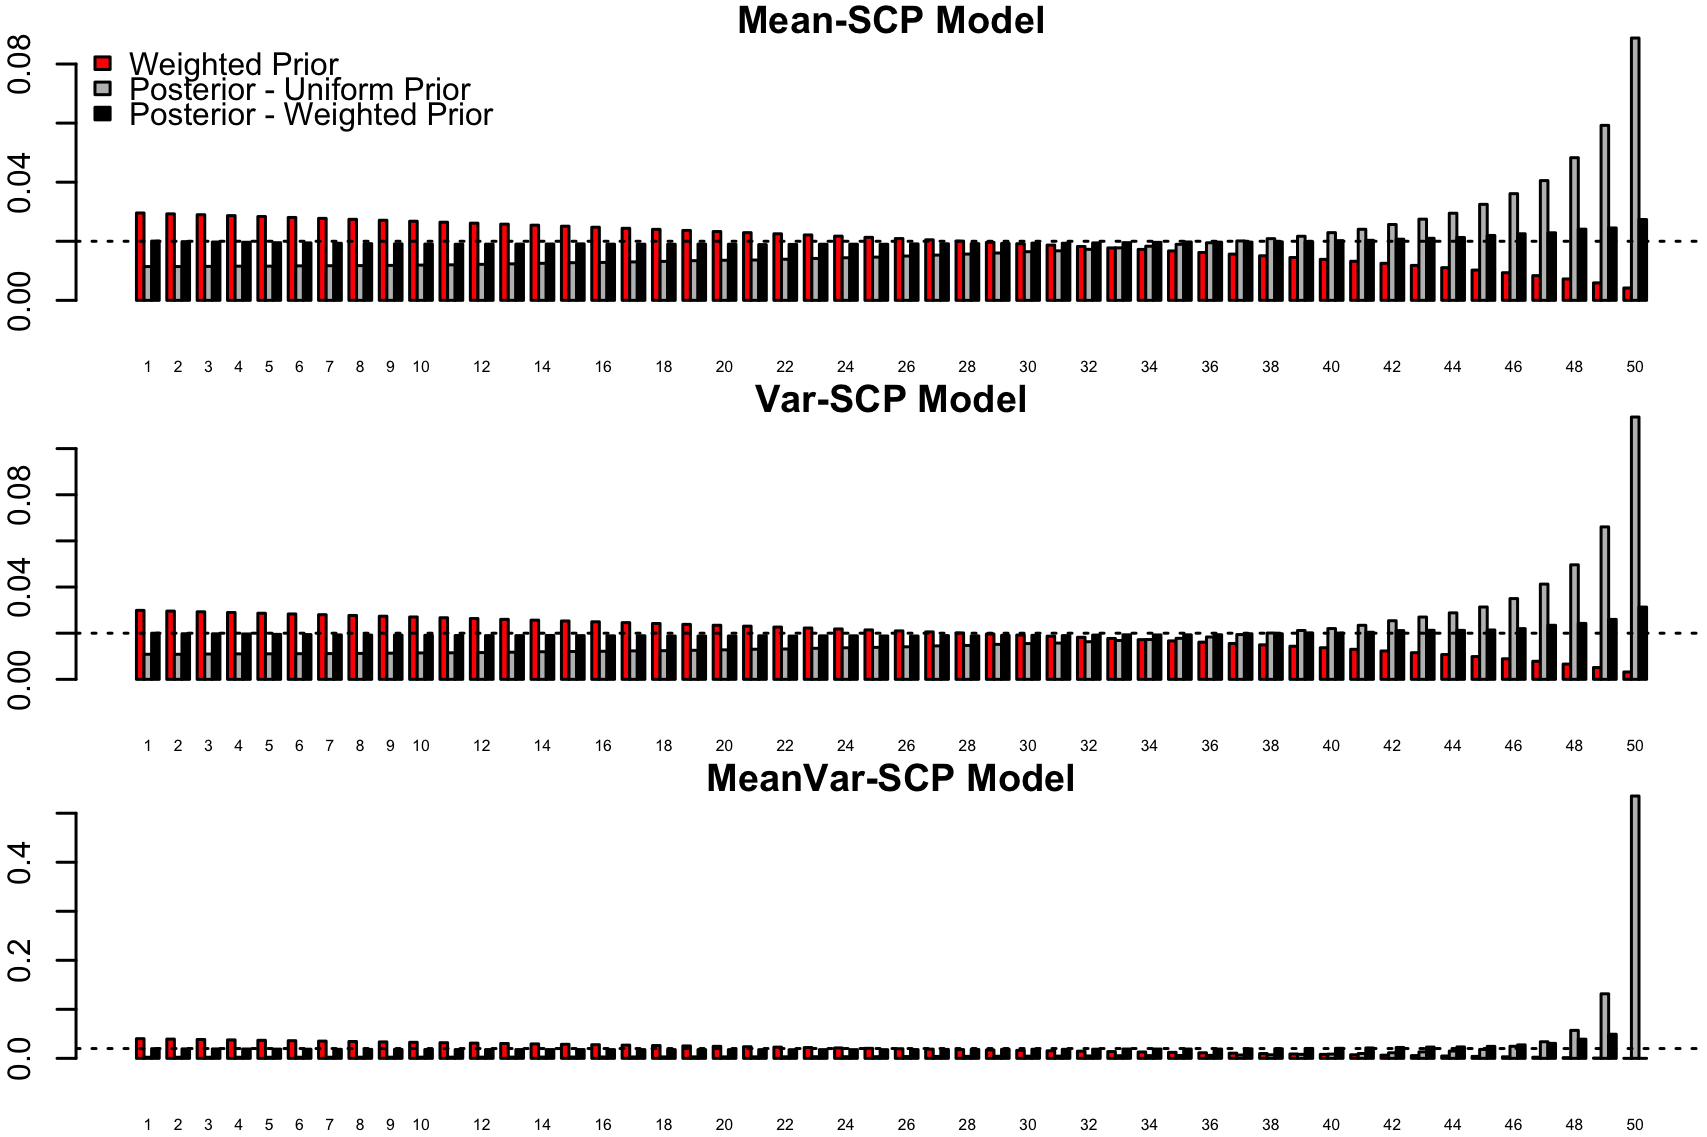
\includegraphics[scale = 0.27]{MICH/Figures/prior_choice_plot.png}
    \caption{$\E[\boldsymbol{\pi}_{1:T}\:|\: \mathbf{y}_{1:T}]$ under Null Model}
    \label{fig:post-probs-plot}
\end{figure}

Figure \ref{fig:post-probs-plot} shows an exponential increase in the posterior probabilities as $t$ approaches $T$. With a uniform prior, the SCP models may fail to detect a true change when the signal is weak or in small samples due to the large weight placed on times near $T$. For the var-scp and meanvar-scp models in particular, we see that the probabilities may be large enough to incorrectly detect a change-point in the vicinity of time $T$, even when no change is present. To rectify this behavior we propose selecting $\boldsymbol{\pi}_{1:T}$ so that under the null model we have:
\begin{align}\label{eq:prior-cond}
    \E\left[\log\overline{\pi}_t - \log \overline{\pi}_{t+1} \right] = 0.
\end{align}
In Figure \ref{fig:post-probs-plot} we also plot the weighted priors $\boldsymbol{\pi}_{1:T}$ that satisfy (\ref{eq:prior-cond}) and MCMC estimates of $\E[\overline{\pi}_{t} \:|\: \mathbf{y}_{1:T}]$ under this choice $\boldsymbol{\pi}_{1:T}$. We clearly see that these estimates adhere much more closely to the uniform dashed line at $T^{-1}$. Note that (\ref{eq:prior-cond}) also implies a uniform condition on the posterior probabilities since for any $r > t$:
\begin{align*}
    \E\left[\log\overline{\pi}_t - \log \overline{\pi}_r \right] &= \sum_{i=0}^{r-t-1} \E\left[\log\overline{\pi}_{t+i} - \log \overline{\pi}_{t+i+1} \right] = 0.
\end{align*}
We now show how to calculate $\pi_t$ so that (\ref{eq:prior-cond}) holds for each of the SCP models. In each case we show that, if $t_0$ is the true location of the change point

\subsubsection{Mean-SCP Prior}

For the mean-scp model in Section \ref{sec:smcp} we have:
\small
\begin{align*}
    \E\left[\log\overline{\pi}_t - \log \overline{\pi}_{t+1} \right] &= \log \pi_t - \log \pi_{t+1} - \frac{1}{2} \log \left|\omega_0\mathbf{I}_d + \sum_{t'=t}^{T} \boldsymbol{\Lambda}_{t'}\right| + \frac{1}{2} \log \left|\omega_0\mathbf{I}_d + \sum_{t'=t+1}^{T} \boldsymbol{\Lambda}_{t'}\right|\\
    &\quad + \frac{1}{2} \E\left[\left\lVert \left[\omega_0\mathbf{I}_d + \sum_{t'=t}^{T} \boldsymbol{\Lambda}_{t'}\right]^{-\frac{1}{2}} \sum_{t'=t}^{T} \boldsymbol{\Lambda}_{t'} \mathbf{y}_{t'}\right\rVert_2^2 \right] - \frac{1}{2} \E\left[\left\lVert \left[\omega_0\mathbf{I}_d + \sum_{t'=t+1}^{T} \boldsymbol{\Lambda}_{t'}\right]^{-\frac{1}{2}} \sum_{t'=t+1}^{T} \boldsymbol{\Lambda}_{t'} \mathbf{y}_{t'}\right\rVert_2^2 \right].
\end{align*}
\normalsize
Letting $\omega_0 \to 0$ and noting that $\sum_{t'=t}^{T} \boldsymbol{\Lambda}_{t'} \mathbf{y}_{t'} \sim \mathcal{N}_d\left(\mathbf{0}, \sum_{t'=t}^{T} \boldsymbol{\Lambda}_{t'}\right)$ under the null model, we get:
\small
\begin{align*}
    \E\left[\log\overline{\pi}_t - \log \overline{\pi}_{t+1} \right] &= \log \pi_t - \log \pi_{t+1} - \frac{1}{2} \log \left|\sum_{t'=t}^{T} \boldsymbol{\Lambda}_{t'}\right| + \frac{1}{2} \log \left|\sum_{t'=t+1}^{T} \boldsymbol{\Lambda}_{t'}\right|\\
    &\quad + \frac{1}{2} \E\left[\left\lVert \left[ \sum_{t'=t}^{T} \boldsymbol{\Lambda}_{t'}\right]^{-\frac{1}{2}} \sum_{t'=t}^{T} \boldsymbol{\Lambda}_{t'} \mathbf{y}_{t'}\right\rVert_2^2  \right] - \frac{1}{2} \E\left[\left\lVert \left[\sum_{t'=t+1}^{T} \boldsymbol{\Lambda}_{t'}\right]^{-\frac{1}{2}} \sum_{t'=t+1}^{T} \boldsymbol{\Lambda}_{t'} \mathbf{y}_{t'}\right\rVert_2^2  \right]\\
    &= \log \pi_t - \log \pi_{t+1} - \frac{1}{2} \log \left|\sum_{t'=t}^{T} \boldsymbol{\Lambda}_{t'}\right| + \frac{1}{2} \log \left|\sum_{t'=t+1}^{T} \boldsymbol{\Lambda}_{t'}\right|.
\end{align*}
\normalsize
If $\boldsymbol{\Lambda}_t = \boldsymbol{\Lambda}$ for all $t$, we can further simplify to:
\begin{align*}
    \E\left[\log\overline{\pi}_t - \log \overline{\pi}_{t+1} \right] &= \log \pi_t - \log \pi_{t+1} + \frac{d}{2} \log\left(\frac{T-t}{T-t+1}\right).
\end{align*}
Therefore, when (\ref{eq:prior-cond}) holds, we can set $\log \pi_1 = 0$ and solve for $\log \pi_t$ for $t > 1$ using the recurrence relation above, then normalize the sequence $\boldsymbol{\pi}_{1:T}$ to get:
\begin{align*}
    \log \pi_t &= \frac{d}{2}\log\left(\frac{T-t+1}{T}\right) - \log\left[\sum_{t'=1}^T \left(\frac{T-t+1}{T}\right)^{\frac{d}{2}}\right] \\
    &\geq - \left(1 + \frac{d}{2}\right)\log T. \tag{$\frac{T-t+1}{T} \leq 1 \sforall t \in [T]$ }
\end{align*}
So for fixed $d$ this choice of $\pi_t$ satisfies Assumption \ref{assumption:1} (iii) with $C_\pi = 1 + \frac{d}{2}$.

\subsubsection{Var-SCP Prior}

For the var-scp model in Section \ref{sec:sscp} we have:
\small
\begin{align*}
    \E\left[\log\overline{\pi}_t - \log \overline{\pi}_{t+1} \right] &= \log \pi_t- \log \pi_{t+1} +\log \Gamma\left(u_0 +\frac{ T-t+1}{2}\right) - \log \Gamma\left(u_0 +\frac{ T-t}{2}\right) + \frac{1}{2} \E[\omega_ty_t^2] \\
    &\quad \: + \left(u_0 + \frac{T - t}{2}\right)\E\left[\log\left[v_0 +\frac{1}{2}\left(\sum_{t'=t+1}^T \omega_{t'}y_{t'}^2\right)\right]\right] \\
     &\quad \:- \left(u_0 + \frac{T - t +1}{2}\right)\E\left[\log\left[v_0 +\frac{1}{2}\left(\sum_{t'=t}^T \omega_{t'}y_{t'}^2\right)\right]\right].
\end{align*}
\normalsize
Letting $u_0,v_0 \to 0$ and noting that $\omega_{t}y^2_{t} \sim \chi^2_1$ under the null model, we get:
\small
\begin{align*}
    \E\left[\log\overline{\pi}_t - \log \overline{\pi}_{t+1} \right] &= \log \pi_t- \log \pi_{t+1} +\log \Gamma\left(\frac{T-t+1}{2}\right) - \log \Gamma\left(\frac{T-t}{2}\right) + \frac{1 + \log 2}{2}\\
    &\quad \: + \left(\frac{T - t}{2}\right)\E\left[\log\left(\sum_{t'=t+1}^T \omega_{t'}y_{t'}^2\right)\right] - \left(\frac{T - t +1}{2}\right)\E\left[\log\left(\sum_{t'=t}^T \omega_{t'}y_{t'}^2\right)\right].
\end{align*}
\normalsize
Since $\sum_{t'=t}^T \omega_{t'}y_{t'}^2 \sim \chi^2_{T-t+1}$, we have:
\begin{align*}
    \E\left[\log\left(\sum_{t'=t}^T \omega_{t'}y_{t'}^2\right)\right] = \psi\left(\frac{T-t+1}{2}\right) + \log 2
\end{align*}
where $\psi$ is the digamma function. Therefore:
\begin{align*}
    \E\left[\log\overline{\pi}_t - \log \overline{\pi}_{t+1} \right] &= \log \pi_t- \log \pi_{t+1} +\log \Gamma\left(\frac{T-t+1}{2}\right) - \log \Gamma\left(\frac{T-t}{2}\right) + \frac{1}{2}\\
    &\quad \: + \left(\frac{T - t}{2}\right)\psi\left(\frac{T-t}{2}\right)  - \left(\frac{T - t +1}{2}\right)\psi\left(\frac{T-t+1}{2}\right).
\end{align*}
So again we have defined a recurrence relation for calculating $\pi_t$. Recall Binet's first formula for the log gamma function for $x > 0$ (see e.g. p. 249 of \citealp{Whittaker96}): 
\begin{align*}
    \log \Gamma(x) = \left(x - \frac{1}{2}\right) \log x - x + \frac{1}{2} \log 2 \pi + \int_{0}^\infty\left(\frac{1}{2} - \frac{1}{t} + \frac{1}{e^t - 1} \right)\frac{e^{-tx}}{t} \;dt.
\end{align*}
Since in Theorem \ref{theorem:sscp} we only consider indexes $t$ such that $T-t+1 > \log^{\varepsilon} T$, we actually only need $\log \pi_t > -C_\pi \log T$ for just these indexes. Since $T-t+1 > \log^{\varepsilon} T \implies T-t+1 \to \infty$, we have the approximations:
\begin{align*}
    \log \Gamma\left(\frac{T-t+1}{2}\right) &\approx \left(\frac{T-t}{2}\right)\log\left(\frac{T - t +1}{2}\right) - \frac{T - t +1}{2} +\frac{1}{2} \log 2 \pi \\
    \psi\left(\frac{T-t+1}{2}\right)  &\approx \log \left(\frac{T-t+1}{2}\right) - \frac{1}{T-t+1}.
\end{align*}
Then we can write:
\begin{align*}
    \E\left[\log\overline{\pi}_t - \log \overline{\pi}_{t+1} \right] &\approx \log \pi_t- \log \pi_{t+1} + \frac{1}{2}\log\left(\frac{T - t}{T-t+1}\right).
\end{align*}
This is the same recurrence relation from the mean-scp model with $d=1$, so again the choice of $\pi_t$ implied by the var-scp recurrence relation satisfies Assumption \ref{assumption:1} (iii).

\subsubsection{MeanVar-SCP Prior}

For the meanvar-scp model in Section \ref{sec:smscp} we have:
\small
\begin{align*}
    \E\left[\log\overline{\pi}_t - \log \overline{\pi}_{t+1} \right] &= \log \pi_t- \log \pi_{t+1} + \frac{1}{2} \E[\omega_ty_t^2] \\
    &\quad \: + \frac{1}{2}\log\left(\sum_{t'=t+1}^T \omega_{t'}\right) - \frac{1}{2}\log\left(\sum_{t'=t}^T \omega_{t'}\right) + \log \Gamma\left(\frac{u_0 + T-t+1}{2}\right) - \log \Gamma\left(\frac{u_0 + T-t}{2}\right)  \\
    &\quad \: + \left(u_0 + \frac{T - t}{2}\right)\E\left[\log\left(v_0 +\frac{1}{2}\sum_{t'=t+1}^T \omega_{t'}y_{t'}^2- \frac{\left(\sum_{t'=t+1}^T \omega_{t'}y_{t'}\right)^2}{2(\omega_0 + \sum_{t'=t+1}^T \omega_{t'})}\right)\right] \\
     &\quad \:- \left(u_0 + \frac{T - t +1}{2}\right)\E\left[\log\left(v_0 +\frac{1}{2}\sum_{t'=t}^T \omega_{t'}y_{t'}^2 - \frac{\left(\sum_{t'=t}^T \omega_{t'}y_{t'}\right)^2}{2(\omega_0 + \sum_{t'=t}^T \omega_{t'})}\right)\right].
\end{align*}
\normalsize
Letting $\omega_0, u_0,v_0 \to 0$ and noting that $\omega_{t}y^2_{t} \sim \chi^2_1$ under the null model, we get:
\small
\begin{align*}
    \E\left[\log\overline{\pi}_t - \log \overline{\pi}_{t+1} \right] &= \log \pi_t- \log \pi_{t+1} + \frac{1 + \log 2}{2} \\
    &\quad \: + \frac{1}{2}\log\left(\sum_{t'=t+1}^T \omega_{t'}\right) - \frac{1}{2}\log\left(\sum_{t'=t}^T \omega_{t'}\right) + \log \Gamma\left(\frac{ T-t+1}{2}\right) - \log \Gamma\left(\frac{T-t}{2}\right)  \\
    &\quad \: + \left(\frac{T - t}{2}\right)\E\left[\log\left(\sum_{t'=t+1}^T \omega_{t'}y_{t'}^2- \frac{\left(\sum_{t'=t+1}^T \omega_{t'}y_{t'}\right)^2}{\sum_{t'=t+1}^T \omega_{t'}}\right)\right] \\
     &\quad \:- \left(\frac{T - t +1}{2}\right)\E\left[\log\left(\sum_{t'=t}^T \omega_{t'}y_{t'}^2 - \frac{\left(\sum_{t'=t}^T \omega_{t'}y_{t'}\right)^2}{\sum_{t'=t}^T \omega_{t'}}\right)\right].
\end{align*}
\normalsize
Noting that the last line above is not well-defined when $t = T$, we can simply set $\pi_T = 0$. Since $\hat{t}_{\text{MAP}} \neq T$ in Theorem \ref{theorem:smscp}, this assumption is without loss of generality. For all other $t \in [T-1]$, since:
\begin{align*}
    \sum_{t'=t}^T \omega_{t'}y_{t'}^2 - \frac{\left(\sum_{t'=t}^T \omega_{t'}y_{t'}\right)^2}{\sum_{t'=t}^T \omega_{t'}} \sim \chi^2_{T-t}
\end{align*}
then we have:
\small
\begin{align*}
    \E\left[\log\overline{\pi}_t - \log \overline{\pi}_{t+1} \right] &= \log \pi_t- \log \pi_{t+1} + \frac{1}{2} + \frac{1}{2}\log\left(\sum_{t'=t+1}^T \omega_{t'}\right) - \frac{1}{2}\log\left(\sum_{t'=t}^T \omega_{t'}\right) \\
    &\quad \:+ \log \Gamma\left(\frac{ T-t+1}{2}\right) - \log \Gamma\left(\frac{T-t}{2}\right)  \\
    &\quad \: + \left(\frac{T - t}{2}\right)\psi\left(\frac{T-t-1}{2}\right) - \left(\frac{T - t +1}{2}\right)\psi\left(\frac{T-t}{2}\right).
\end{align*}
\normalsize
So again we have defined a recurrence relation for calculating $\pi_t$. Since $\boldsymbol{\tau}_{1:T}$ are known parameters, it is without loss of generality to assume that $\omega_t = 1$, then we have:   
then we have:
\small
\begin{align*}
    \E\left[\log\overline{\pi}_t - \log \overline{\pi}_{t+1} \right] &= \log \pi_t- \log \pi_{t+1} + \frac{1}{2} + \frac{1}{2}\log\left(\frac{T-t}{T-t+1}\right) + \log \Gamma\left(\frac{ T-t+1}{2}\right) - \log \Gamma\left(\frac{T-t}{2}\right)  \\
    &\quad \: + \left(\frac{T - t}{2}\right)\psi\left(\frac{T-t-1}{2}\right) - \left(\frac{T - t +1}{2}\right)\psi\left(\frac{T-t}{2}\right).
\end{align*}
\normalsize
Noting that the right hand side is just a sum of the recurrence relations for the mean-scp and var-scp models, then we can use the same argument that we used in those previous cases to establish that the choice of $\pi_t$ implied by the meanvar-scp recurrence relation satisfies Assumption \ref{assumption:1} (iii).

\normalsize

\subsection{Merging Duplicate Components}
\label{app:merge-procedure}

As discussed in Section \ref{sec:merge-procedure}, Algorithm \ref{alg:1} occasionally reaches a stationary point where a single change-point is split across multiple $\gamma_i$'s. We propose a modification that helps Algorithm \ref{alg:1} move out of theses stationary points. If $\gamma_i$ and $\gamma_{i'}$ correspond to change-points of the same class, then by (\ref{eq:mean-field}) we have:
\begin{align}
    q(\gamma_i = \gamma_{i'}) = \sum_{t=1}^T q(\gamma_{i'} = t | \gamma_i = t ) q(\gamma_i = t) = \sum_{t=1}^T q_{i'}(\gamma_{i'} = t)q_i(\gamma_i = t) = \langle\overline{\boldsymbol{\pi}}_{i'}, \overline{\boldsymbol{\pi}}_i \rangle.
\end{align}
We therefore propose merging components $i$ and $i'$ if $\langle\overline{\boldsymbol{\pi}}_{i'}, \overline{\boldsymbol{\pi}}_i \rangle$ exceeds some threshold $\beta > 0$. In the event that $\min\{\langle\overline{\boldsymbol{\pi}}_{i'}, \overline{\boldsymbol{\pi}}_i \rangle,\langle\overline{\boldsymbol{\pi}}_{i'}, \overline{\boldsymbol{\pi}}_{i''} \rangle\} \geq \beta$, but $\langle\overline{\boldsymbol{\pi}}_{i}, \overline{\boldsymbol{\pi}}_{i''} \rangle \leq \beta$, we enforce transitivity and merge components $i$, $i'$, and $i''$. When components $i$ and $i'$ both capture true change-points, then $\overline{\boldsymbol{\pi}}_{i}$ and $\overline{\boldsymbol{\pi}}_{i'}$ tend to be sparse. Thus, when components $i$ and $i'$ correspond to distinct change-points, $\langle\overline{\boldsymbol{\pi}}_{i}, \overline{\boldsymbol{\pi}}_{i'} \rangle$ tends to be vanishingly small. When components $i$ and $i'$ capture the same change-point, $\langle\overline{\boldsymbol{\pi}}_{i}, \overline{\boldsymbol{\pi}}_{i'}\rangle$ will clearly be nonzero in most cases, so any small value of $\beta$ will correctly merge the true duplicates. After merging the duplicate components, we then restart Algorithm \ref{alg:1}. To account for the fact that Algorithm \ref{alg:1} may just split the merged components again, we iteratively increase $\beta$ until no more merges are proposed, which prevents the procedure from entering an infinite loop. 

To select a default for $\beta$, we consider the worst case scenario where $t^*_i$ and $t^*_{i+1}$ are consecutive change-points separated by the minimum spacing condition from Assumption \ref{assumption:1}, i.e. $|t^*_i - t^*_{i+1}| = \log^{1+\varepsilon} T$ for some $\varepsilon > 0$. Suppose components $i$ and $i+1$ of MICH identify $t^*_i$ and $t^*_{i+1}$ respectively. Given a localization rate $\epsilon_T = \mathcal{O}(\log T)$, for large enough $T$ we have $\mathbb{B}_{\epsilon_T}^{1}(t^*_i) \cap \mathbb{B}_{\epsilon_T}^{1}(t^*_{i+1}) = \emptyset$. In the proof of Corollary \ref{cor:cred-sets}, we show that $\overline{\pi}_{it} \leq T^{-2}$ with high probability for $t \not\in \mathbb{B}_{\epsilon_T}^{1}(t^*_i)$. Though this result is for the single change-point setting, in empirical results for the multiple change-point setting, we observe a similar rate of decay for the posterior probabilities that fall outside of the window defined by the localization rate. Thus, with high probability:
\begin{align}
    \sum_{t \in \mathbb{B}_{\epsilon_T}^{1}(t^*_{i+1})} \overline{\pi}_{it} \overline{\pi}_{(i+1)t} \leq \frac{2\epsilon_T}{T^2}
\end{align}
A symmetric argument gives an identical bound for $t \in \mathbb{B}_{\epsilon_T}^{1}(t^*_{i})$, and for the remaining indices we have $\overline{\pi}_{it} \overline{\pi}_{(i+1)t} \leq T^{-4}$; therefore, the merge probability in this case is at most $\mathcal{O}(T^{-2}\log T)$. If we set $\beta = \frac{\log^{2+\delta} T}{T^2}$, where $\delta > 0$ is the same value used in the detection rule (\ref{eq:LKJ-estimator}), then we should avoid merging any truly distinct components with high probability as $T \to \infty$.

The merge procedure we have proposed may still run into issues when the model includes redundant components. As previously noted, when component $i$ does not capture a change-point, then $\overline{\boldsymbol{\pi}}_{i}$ tends to be diffuse with $\overline{\pi}_{it} \approx T^{-1}$. If component $i'$ does correspond to a change and $\overline{\boldsymbol{\pi}}_{i'}$ is sparse, then we may end up with a situation where $\langle\overline{\boldsymbol{\pi}}_{i}, \overline{\boldsymbol{\pi}}_{i'}\rangle \approx T^{-1}$. Under the default value of $\beta$ we have proposed, components $i$ and $i'$ will be erroneously merged. To avoid this outcome, we only merge components that we believe detect true change-points, i.e. we restrict merge candidates to only include the model components with $\alpha$-level credible sets that satisfy the detection rule (\ref{eq:LKJ-estimator}) with $\alpha = 0.9$ by default. The procedure tends to be insensitive to the choice of $\alpha$, so long as it is moderately large. For example, when $T = 100$, we have $\log^2 T \approx 25$, so for a diffuse $\overline{\boldsymbol{\pi}}_i$, we would rule component $i$ out as a merge candidate for any $\alpha \geq 0.25$.


\section{Plots and Figures}

\subsection{Plate Diagram of MICH}
\label{app:plate-diagram}

\begin{figure}
    \centering
    \begin{tikzpicture}[x=1.7cm,y=1.8cm]
  % Nodes

  % DGP
  \node[obs]                   (y)      {$y_t$} ; 
  \factor[above=0.76cm of y] {y-f} {above:$\mathcal{N}$} {} {} ; %
  \node[latent, above=0.5cm of y, xshift = -2cm]    (mu)     {$\mu_t$} ; 
  \node[latent, above=0.5cm of y, xshift = 2cm]    (lambda) {$\lambda_t$} ; 

  % SMCP
  \node[latent, left=0.5 of mu] (b_l) {$b_\ell$} ;
  \factor[left=of b_l, xshift=0.25cm] {b_l-f} {above:$\mathcal{N}$} {} {} ; %
  \node[const, left=of b_l, xshift=0.75cm] (tau_l) {$\tau_\ell$} ; %

  \node[latent, left=0.5 of mu, yshift=1cm] (gamma_l) {$\gamma_\ell$} ;
  \factor[left=of gamma_l, xshift=0.25cm] {gamma_l-f} {above:Multi.} {} {} ; %
  \node[const, left=of gamma_l, xshift=0.75cm] (pi_l) {$\pi_\ell$} ; %

  % SSCP
  \node[latent, right=0.5 of lambda] (s_k) {$s_k$} ;
  \factor[right=of s_k, xshift=-0.25cm] {s_k-f} {above:$\mathcal{G}$} {} {} ; %
  \node[const, right=of s_k, xshift=-0.75cm, yshift = 0.5cm] (u_k) {$u_k$} ; %
  \node[const, right=of s_k, xshift=-0.75cm, yshift = -0.5cm] (v_k) {$v_k$} ; %

  \node[latent, right=0.5 of lambda, yshift=1cm] (gamma_k) {$\gamma_k$} ;
  \factor[right=of gamma_k, xshift=-0.25cm] {gamma_k-f} {above:Multi.} {} {} ; %
  \node[const, right=of gamma_k, xshift=-0.75cm] (pi_k) {$\pi_k$} ; %

  % SMSCP
  \node[latent, above=2cm of mu] (b_j) {$b_j$} ;
  \node[latent, above=2cm of lambda] (s_j) {$s_j$} ;
  \factor[above=0.2 of s_j, xshift=0cm] {s_j-f} {left:$\mathcal{G}$} {} {} ; %
  \node[const, above=0.5 of s_j, xshift=-0.25cm] (u_j) {$u_j$} ; %
  \node[const, above=0.5 of s_j, xshift=0.2cm] (v_j) {$v_j$} ; %
  
  \node[latent, above=1.2cm of y-f] (gamma_j) {$\gamma_j$} ;
  \factor[above=0.61cm of gamma_j] {b_j-f} {below:$\mathcal{N}$} {} {} ; %
  \node[const, above=0.65cm of b_j-f] (tau_j) {$\tau_j$} ; %
  \factor[left=of gamma_j , xshift=0.3cm] {gamma_j-f} {above:Multi.} {} {} ; %
  \node[const, left=of gamma_j, xshift=0.8cm] (pi_j) {$\pi_j$} ; %

  % Connect the nodes
  \edge {y-f} {y} ;
  \edge[-] {mu, lambda} {y-f} ; %

  \edge{gamma_l, b_l} {mu}
  \edge[-] {b_l-f} {b_l} ; %
  \edge[-] {gamma_l-f} {gamma_l} ; %
  \edge[-] {tau_l} {b_l-f} ; %
  \edge[-] {pi_l} {gamma_l-f} ; %

  \edge{gamma_k, s_k} {lambda}
  \edge[-] {s_k-f} {s_k} ; %
  \edge[-] {gamma_k-f} {gamma_k} ; %
  \edge[-] {u_k, v_k} {s_k-f} ; %
  \edge[-] {pi_k} {gamma_k-f} ; %

  
  \edge{gamma_j, b_j} {mu}
  \edge{b_j-f} {b_j} ; %
  \edge[-] {tau_j,s_j} {b_j-f} ; %
  \edge[-] {gamma_j-f} {gamma_j} ; %
  \edge[-] {pi_j} {gamma_j-f} ; %
  \edge{gamma_j, s_j} {lambda}
  \edge[-] {s_j-f} {s_j} ; %
  \edge[-] {u_j, v_j} {s_j-f} ; %
  
  % Plates
  \plate[thick, inner sep=.25cm]{y} {(y)(mu)(lambda)} {$1 -B_l \leq t \leq T+B_r$} ;
  \tikzset{plate caption/.append style={above right =0pt of #1.north west}}
  \plate[thick,color=violet]{mu lambda} {(mu)(lambda)(gamma_j)(gamma_j-f)(pi_j)(b_j)(b_j-f)(tau_j)(s_j)(s_j-f)(u_j)(v_j)}{\textcolor{violet}{$1 \leq j \leq J$}} ;
  \tikzset{plate caption/.append style={below left = 5pt of #1.south east}}
  \plate[thick,color=red]{lambda} {(lambda)(gamma_k)(gamma_k-f)(pi_k)(s_k)(s_k-f)(u_k)(v_k)}{\textcolor{red}{$1 \leq k \leq K$}} ;
  \tikzset{plate caption/.append style={below=10pt of #1.south west, xshift=0.75cm}}
  \plate[thick,color=blue]{mu} {(mu)(gamma_l)(gamma_l-f)(pi_l)(b_l)(b_l-f)(tau_l)}{\textcolor{blue}{$1 \leq \ell \leq L$}} ;
\end{tikzpicture}
    \caption{Plate diagram depicting the directed acyclic graph specified by (\ref{eq:dgp}) and (\ref{eq:mu_t})-(\ref{eq:lambda_t}).}
    \label{fig:plate-diagram}
\end{figure}

